\documentclass[11pt,oneside]{book}
\usepackage{fontspec}
\usepackage{xeCJK}
\setmainfont{Latin Modern Roman}
\setCJKmainfont[ItalicFont={Noto Serif CJK TC},BoldItalicFont={Noto Serif CJK TC Bold}]{Noto Serif CJK TC}
\setCJKsansfont{Noto Sans CJK TC}
\setCJKmonofont{Noto Sans Mono CJK TC}
\newfontfamily\proseunicodefont{DejaVu Serif}
\usepackage[margin=1in]{geometry}
\usepackage{microtype}
\usepackage{amsmath,amssymb,amsthm,mathtools,bm}
\usepackage{graphicx}
\usepackage{xcolor}
\usepackage{booktabs}
\usepackage{array}
\usepackage{longtable}
\usepackage{enumitem}
\usepackage{float}
\usepackage{caption}
\usepackage{hyperref}
\usepackage{fancyhdr}
\usepackage{tikz}
\usetikzlibrary{arrows.meta,positioning,calc,decorations.pathmorphing}

\hypersetup{
  colorlinks=true,
  linkcolor=blue!50!black,
  urlcolor=blue!50!black,
  citecolor=blue!50!black
}

\setlength{\parskip}{0.5em}
\setlength{\parindent}{0pt}
\setlist[itemize]{topsep=0.25em,itemsep=0.2em}
\setlist[enumerate]{topsep=0.25em,itemsep=0.2em}
\setlength{\headheight}{40pt}
\numberwithin{equation}{chapter}

\newtheorem{theorem}{定理}[chapter]
\newtheorem{proposition}[theorem]{命題}
\newtheorem{lemma}[theorem]{引理}
\newtheorem{corollary}[theorem]{推論}
\theoremstyle{definition}
\newtheorem{definition}[theorem]{定義}
\newtheorem{example}[theorem]{例}
\theoremstyle{remark}
\newtheorem{remark}[theorem]{註}

\providecommand{\ket}[1]{\left\lvert#1\right\rangle}
\providecommand{\bra}[1]{\left\langle#1\right\rvert}
\providecommand{\braket}[2]{\left\langle#1\,\middle|\,#2\right\rangle}
\providecommand{\expect}[1]{\left\langle#1\right\rangle}
\newcommand{\lectureoverview}[1]{\paragraph{概述。} #1}
\newenvironment{classroomqa}{%
  \par\medskip
  \begin{quote}\small
}{%
  \end{quote}
  \medskip
}
\newcommand{\audiencequestion}[1]{\noindent\textbf{聽眾提問。} #1\par\smallskip}
\newcommand{\classquestion}[1]{\noindent\textbf{課堂提問。} #1\par\smallskip}
\newcommand{\lecturerresponse}[1]{\noindent\textbf{回答。} #1\par}
\newcommand{\lecturetimestamp}[1]{\footnote{講課時間： #1.}}
\newcommand{\lectureframe}[1]{\par\smallskip{\centering\footnotesize\itshape 講課畫面： #1.\par}}

\makeatletter
\newcommand{\course@headerfont}{\normalfont\small\itshape}
\newcommand{\course@pagefont}{\normalfont\small}
\newcommand{\course@headerraise}{14pt}
\newlength{\course@headerboxheight}
\setlength{\course@headerboxheight}{\dimexpr\headheight-\course@headerraise-9pt\relax}
\newcommand{\course@leftheadbox}[1]{%
  \raisebox{\course@headerraise}{%
    \parbox[t][\course@headerboxheight][t]{0.82\textwidth}{%
      \raggedright\course@headerfont\strut\MakeUppercase{#1}\strut%
    }%
  }%
}
\newcommand{\course@rightheadbox}[1]{%
  \raisebox{\course@headerraise}{%
    \parbox[t][\course@headerboxheight][t]{0.82\textwidth}{%
      \raggedleft\course@headerfont\strut\MakeUppercase{#1}\strut%
    }%
  }%
}
\renewcommand{\chaptermark}[1]{\markboth{\MakeUppercase{\chaptername\ \thechapter.\ #1}}{}}
\renewcommand{\sectionmark}[1]{\markright{\MakeUppercase{\thesection\hspace{0.4em}#1}}}
\fancyhf{}
\fancyhead[L]{\course@leftheadbox{\leftmark}}
\fancyhead[R]{\course@pagefont\thepage}
\renewcommand{\headrulewidth}{0.5pt}
\pagestyle{fancy}
\fancypagestyle{plain}{%
  \fancyhf{}
  \fancyhead[L]{\course@leftheadbox{\leftmark}}
  \fancyhead[R]{\course@pagefont\thepage}
  \renewcommand{\headrulewidth}{0.5pt}
}
\makeatother

\renewcommand{\contentsname}{目錄}
\renewcommand{\chaptername}{章}
\renewcommand{\figurename}{圖}
\renewcommand{\tablename}{表}
\renewcommand{\proofname}{證明}
\renewcommand{\bibname}{參考文獻}
\emergencystretch=2em
\pdfstringdefDisableCommands{\def\proseunicodefont{}}

\geometry{paperwidth=177.6mm,paperheight=252mm,left=16mm,right=16mm,
 top=18mm,bottom=18mm,includeheadfoot,headheight=28pt,headsep=7mm,footskip=9mm}
\usepackage{scrextend}
\changefontsizes[17pt]{12pt}
\raggedbottom
\renewenvironment{classroomqa}{\par\medskip\begingroup}{\par\endgroup\medskip}
\fancyhf{}
\setlength{\headwidth}{\textwidth}
\fancyhead[L]{\parbox{\textwidth}{\raggedright\fontsize{9}{11}\selectfont\nouppercase{\leftmark}}}
\fancyfoot[C]{\small\thepage}
\renewcommand{\headrulewidth}{0.3pt}
\fancypagestyle{plain}{\fancyhf{}\fancyfoot[C]{\small\thepage}\renewcommand{\headrulewidth}{0pt}}

\graphicspath{{../../../generated_course_notes/core/statistical_mechanics/2013_spring_theoretical_minimum/figures/}{../../../generated_course_notes/core/statistical_mechanics/2013_spring_theoretical_minimum/assets/}}
\hypersetup{
  pdftitle={Statistical Mechanics: The Theoretical Minimum},
  pdfauthor={Leonard Susskind; companion notes edited by LazyingArt LLC with Video2Book},
  pdfsubject={Core track, 2013 Spring},
  pdfkeywords={Leonard Susskind, statistical mechanics, thermodynamics, Ising model, critical phenomena}
}
\begin{document}
\frontmatter
\hypersetup{pageanchor=false}
\begin{titlepage}
\hyphenpenalty=10000\exhyphenpenalty=10000
\thispagestyle{empty}
\begin{tikzpicture}[remember picture,overlay]
  \node[anchor=south west,inner sep=0] at (current page.south west) {%
    \includegraphics[width=\paperwidth,height=\paperheight,keepaspectratio=false]{../../../generated_course_notes/core/statistical_mechanics/2013_spring_theoretical_minimum/assets/cover-art.png}%
  };
  \node[
    anchor=north west,
    align=left,
    text width=0.78\paperwidth,
    fill=white,
    fill opacity=0.9,
    rounded corners=8pt,
    inner xsep=10pt,
    inner ysep=8pt
  ] at ([xshift=0.08\paperwidth,yshift=-0.06\paperheight]current page.north west) {%
    {\fontsize{30}{33}\selectfont\bfseries\color{black!88} 統計力學\\[0.85em]}
    {\large\color{black!72} 繁體中文版 / 2013年春季・理論最低限度}
  };
  \node[
    anchor=south west,
    align=left,
    text width=0.68\paperwidth,
    fill=white,
    fill opacity=0.82,
    text opacity=1,
    rounded corners=6pt,
    inner sep=12pt
  ] at ([xshift=0.08\paperwidth,yshift=0.08\paperheight]current page.south west) {%
    {\normalsize\color{black!78} 原講授：Leonard Susskind\\[0.35em]}
    {\small\color{black!72} 講義輔助版本：\href{https://lazying.art}{LazyingArt LLC} / \href{https://github.com/lachlanchen/Video2Book}{Video2Book}.}
  };
\end{tikzpicture}
\mbox{}
\end{titlepage}
\hypersetup{pageanchor=true}

\chapter*{關於本講義}
這套經獨立編輯的配套講義，依據 Leonard Susskind 的 2013 年《統計力學》課程講授內容編寫。講義保留了課程的講解順序、實質的課堂交流、數學推導，以及部分黑板內容紀錄。這不是 Susskind 教授的原稿，也未經他審閱或認可。

本版本由 \href{https://lazying.art}{LazyingArt LLC} 採用開源的 \href{https://github.com/lachlanchen/Video2Book}{Video2Book} 工作流程編製。完整的機器轉錄稿與字幕檔另存於程式碼儲存庫中，其中可能含有辨識錯誤。
\clearpage
\tableofcontents
\mainmatter
\chapter{機率、資訊與熵}

\lectureoverview{統計力學始於微觀定律與不完備知識交會之處。我們先明確定義機率，再探討確定性運動本身如何賦予機率、守恆定律如何劃分狀態空間，以及為何保留資訊的動力學自然導向熵。等這套架構建立起來之後，才會談到第一定律與第零定律。}

\section{為什麼需要統計力學？}

統計力學有時被稱為舊物理學。這種說法沒有抓住重點。它既屬於前現代，也屬於現代，而且很可能在任何承接我們現有理論的後現代物理學中繼續發揮作用。具體模型不斷更迭；熱力學第二定律卻一再經受考驗，持續為我們指引方向。每當某種自然描述看似能憑空創造秩序、從根本上抹除資訊，或使封閉系統走向不自然的簡單狀態，第二定律便提醒我們：其中必定遺漏了某些因素。

這門學科或許不如新發現的粒子那樣引人注目，卻至少同樣深刻，而且普遍得多。氣體、液體、固體、輻射、黑洞、資訊和量子場，都需要統計推理。事實上，若不了解統計力學，就無法理解用來發現粒子的實驗設備。這也就是為什麼一代又一代傑出的物理學家，即使主要研究其他領域，也都精通統計力學：它不只實用，而且格外優美。

要了解為什麼需要統計力學，可以先從力學所提供的理想情形談起。封閉系統可以是我們所考慮的整個宇宙，也可以是隔離得足夠完善、因而不受周遭環境影響的子系統。如果知道它的初始條件和演化定律，經典力學便能給出完整的預測。量子力學改變了可預測的內容，但同樣具有明確定義的狀態，以及一條能預測該理論所容許最大資訊的定律。

原則上能夠預測，與實際上能夠理解，兩者相差甚遠。若列出這個房間裡每個分子的位置和速度，清單將長得驚人，幾乎立刻就會改變，而且幾乎回答不了我們真正關心的問題。因此，精確的微觀定律可以同時完全具備預測力，卻在實際應用上毫無用處。

統計力學是將機率論應用於這種物理情境。當初始條件無法完全精確得知、定律只能近似得知、系統是開放的，或單純因為微觀變數多到無法追蹤時，統計力學就不可或缺。這些情況都不代表預測能力薄弱。大量元素往往反而讓統計預測變得極為精確。

考慮一個孤立的氣體盒子。我們無法預測每個分子的軌跡，但只要少數宏觀資料，就能高精度地預測壓力、能量和許多其他宏觀量。仍然無法確定的是漲落。在某個不可預測的時刻，一小塊區域裡的分子可能多於平均值，而另一塊則可能少於平均值。這種事件落在機率分佈的尾端：機率低，但並非不可能。我們可以計算這類漲落應出現的頻率，卻無法預測某一次漲落會在什麼時刻發生。

擲硬幣也呈現相同的區別。公平地擲十億次，正面和反面的次數會相當接近。只要擲得夠多次，終究會出現一連串正面；但機率論預測的是它出現的頻率，而不是事先指定它何時發生。統計力學是為元素太小、太多，或兩者兼具的系統而設的。

本課程將介紹這些定律，以及它們在物質上的應用。這門學科值得反覆研習：學會之後，可能忘掉其中一些部分，再重新學習時，便會更深刻地體會哪些觀念才是根本。我們先從支配後續一切內容的觀念談起。

\section{作為基本語言的機率}

機率為何有效，並不是機率演算本身所能解釋的。機率預測可能在某一次試驗中失準；可能發生卻不太可能發生的結果，正是這個意思。理論告訴我們例外如何分佈，但不會讓例外消失。因此，我們把機率視為基本概念，並列出它所遵循的規則。

\subsection{狀態與歸一化}

令\(i\)表示一個可能的結果或系統的一種可能狀態。對一枚硬幣而言，\(i\)可以表示正面或反面。對一顆骰子而言，它可以從\(1\)到\(6\)。對兩顆骰子而言，一對指標可以記錄兩顆骰子的點數。我們先考慮有限的離散狀態空間，
\begin{equation}
 i=1,\ldots,N,
\end{equation}
之後再推廣到無限多個狀態，以及連續的狀態。

無知不代表系統沒有狀態，而是代表我們不知道它處於哪個狀態，因此對每種可能性都指定一個機率\(p_i\)。基本規則如下：
\begin{align}
 p_i &\geq 0, \label{eq:sm1-prob-positive}\\
 \sum_{i=1}^{N}p_i &=1. \label{eq:sm1-prob-normalization}
\end{align}
各種可能性彼此互斥，而且涵蓋所有情形：其中恰好有一種會發生。這裡不會有負機率，機率總和為一，因為某個允許的結果必定會發生。

\subsection{頻率與大數定律}

機率透過重複試驗與實驗相連。假設同一實驗進行\(N_{\mathrm{trials}}\)次，令\(N(i)\)表示結果\(i\)出現的試驗次數。頻率詮釋如下：
\begin{equation}
 p_i=
 \lim_{N_{\mathrm{trials}}\to\infty}
 \frac{N(i)}{N_{\mathrm{trials}}}.
 \label{eq:sm1-frequency}
\end{equation}
這是一項以理想極限表達的物理假設。沒有實驗室能進行無限多次實驗。這項主張是：試驗次數足夠多時，比值會穩定在足夠接近\(p_i\)的範圍內，以符合預期的預測。有限樣本的頻率會在極限值附近漲落。

\subsection{平均值}

現在為每個狀態指定一個數值\(f(i)\)。它可以是能量、動量，或任何我們想測量的量。其期望值為
\begin{equation}
 \langle f\rangle=\sum_i f(i)p_i.
 \label{eq:sm1-expectation}
\end{equation}
即使在量子力學之外，使用括號記號也很方便。以頻率來表示，同一個平均值為
\begin{equation}
 \langle f\rangle
 =
 \lim_{N_{\mathrm{trials}}\to\infty}
 \frac{1}{N_{\mathrm{trials}}}
 \sum_i f(i)N(i).
 \label{eq:sm1-frequency-average}
\end{equation}

對一枚硬幣，定義
\begin{equation}
 f(\mathrm{H})=+1,
 \qquad
 f(\mathrm{T})=-1.
\end{equation}
若正面和反面的機率各為\(1/2\)，則
\begin{equation}
 \langle f\rangle
 =(+1)\frac12+(-1)\frac12=0.
\end{equation}
平均值不一定是可能出現的結果。硬幣不會落在零上；零只是概括了兩種可能取值的分佈。

這段簡短的插曲確立了本學科通篇使用的詞彙：狀態、機率、頻率和期望值。

\section{指定機率的三種方式}

\subsection{對稱性}

為什麼我們通常給硬幣的兩面相同的機率？第一個答案是對稱性。翻轉一枚近乎理想的硬幣，正面和反面會互換，但實驗本身不變。因此，沒有物理理由偏向任何一種結果。真實的標記或瑕疵會引入微小偏差，但對稱模型足以描述我們所設想的實驗：
\begin{equation}
 p(\mathrm{H})=p(\mathrm{T})=\frac12.
\end{equation}

同樣的推理也會給對稱骰子的每一面指定機率\(1/6\)。更一般地說，除非有額外資訊打破對稱性，否則由對稱性相互關聯的構型會被指定相同的機率。

\subsection{實驗}

形狀不規則的骰子沒有能互換全部六面的對稱性。在這種情況下，光靠對稱性無法得出答案。或許有更深入的力學模型能預測偏差；但若沒有這樣的模型，誠實的做法就是進行實驗：多次擲骰，記錄頻率，等頻率趨於穩定，再用所得的機率表進行後續預測。

對稱性和實驗並非互相競爭的定義，而是取得機率分佈資訊的兩種途徑。統計力學會大量運用對稱性，而動力學則提供第三種途徑。

\subsection{從確定性運動得出機率}

想像一個不規則物體，有六種不同顏色的構型。它依照確定的更新規則，每隔固定的離散時間改變一次狀態：
\begin{equation}
 R\longrightarrow B\longrightarrow Y\longrightarrow G
 \longrightarrow O\longrightarrow P\longrightarrow R.
 \label{eq:sm1-six-cycle}
\end{equation}
物體本身不必具有任何幾何對稱性。這條規則只說明某個構型之後會接續哪個構型。

\begin{figure}[htbp]
\centering
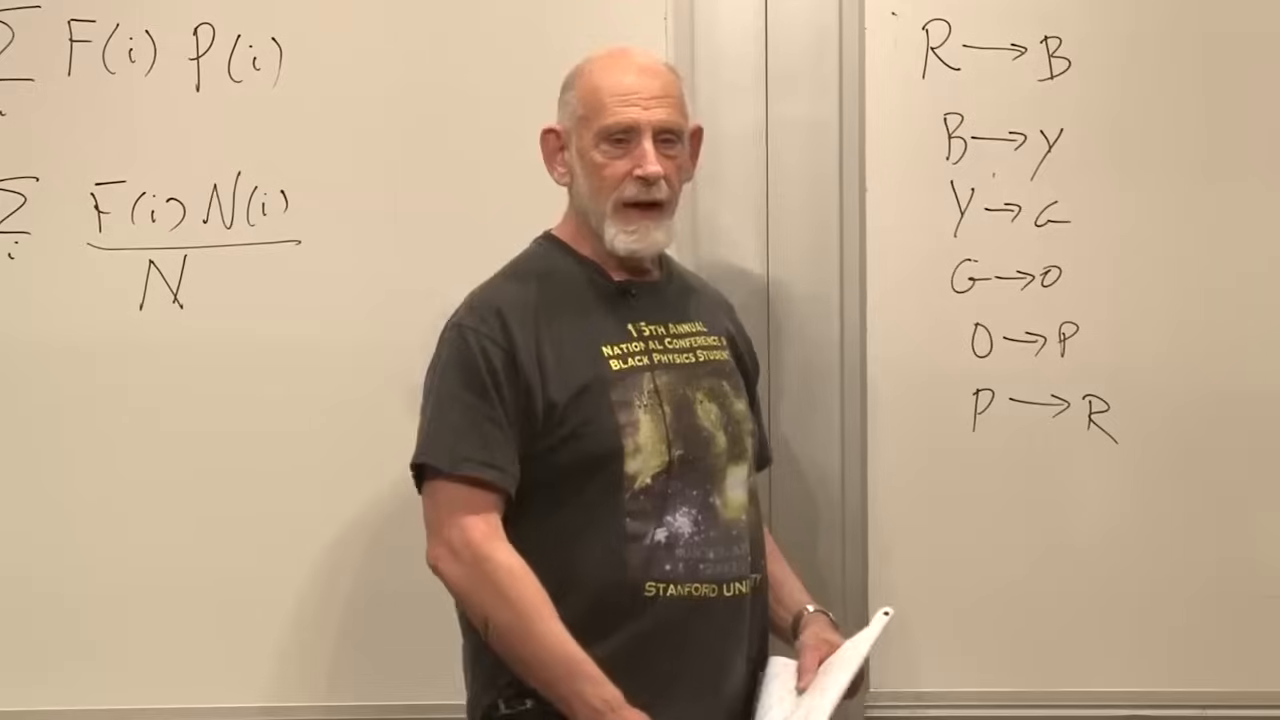
\includegraphics[width=0.92\textwidth]{lecture_01_figure_02.png}
\caption{左側黑板保留期望值公式，右側則列出六種顏色狀態的確定性更新規則。}
\lectureframe{00:26:28}
\end{figure}

若將黑板上的列表畫成有向迴圈，關係會更清楚：
\begin{figure}[htbp]
\centering
\begin{tikzpicture}[
  >=Latex,
  state/.style={draw,circle,minimum size=8mm,inner sep=1pt}
]
\node[state] (R) at (90:2.2) {$R$};
\node[state] (B) at (30:2.2) {$B$};
\node[state] (Y) at (-30:2.2) {$Y$};
\node[state] (G) at (-90:2.2) {$G$};
\node[state] (O) at (-150:2.2) {$O$};
\node[state] (P) at (150:2.2) {$P$};
\draw[->] (R) -- (B);
\draw[->] (B) -- (Y);
\draw[->] (Y) -- (G);
\draw[->] (G) -- (O);
\draw[->] (O) -- (P);
\draw[->] (P) -- (R);
\end{tikzpicture}
\caption{一個由六個狀態組成的單一軌道。每個週期中，每種狀態都會經過一次。}
\label{fig:sm1-six-cycle}
\end{figure}

假設我們不知道初始狀態，並在未知時刻拍下一張快照。由於每一步持續時間相同，系統在每種顏色狀態停留的時間都是一個週期的六分之一：
\begin{equation}
 p(R)=p(B)=p(Y)=p(G)=p(O)=p(P)=\frac16.
 \label{eq:sm1-uniform-cycle}
\end{equation}
這種均等並非來自物體的形狀，而是來自系統在各狀態中停留的時間相同。

我們可以重新排列箭頭，形成一條不同的微觀定律，但仍然是一個由六個狀態組成的迴圈。狀態的先後順序改變了，但快照機率仍是\(1/6\)，因為每個週期中仍會經過每種狀態一次。因此，這項預測既不需要知道起點，也不需要知道具體的先後順序；只要知道軌道結構，以及每次更新所對應的時間相同即可。

\begin{classroomqa}
\classquestion{如果物體並不對稱，給每種顏色指定機率\(1/6\)，在什麼意義上才合理？}
\lecturerresponse{這種指定依據的是動力學，而不是幾何。若在六步軌道的未知相位拍下快照，取樣的就是六個等長的時間區間。相關的等價性存在於軌道上的各個位置之間，而不在物體的各面之間。若停留時間不相等，機率也會不相等。
\lecturetimestamp{00:27:11--00:29:49}}
\end{classroomqa}

\section{不連通的迴圈與守恆量}

確定性定律不一定會讓所有狀態都落在同一條軌道上。考慮兩條彼此不連通的迴圈：
\begin{equation}
 R\longrightarrow B\longrightarrow G\longrightarrow R,
 \qquad
 P\longrightarrow Y\longrightarrow O\longrightarrow P.
 \label{eq:sm1-two-cycles}
\end{equation}
如果知道系統位於第一條迴圈上，那麼
\begin{equation}
 \begin{aligned}
 p(R)=p(B)=p(G)&=\frac13,\\
 p(P)=p(Y)=p(O)&=0.
 \end{aligned}
\end{equation}
若知道它位於第二條迴圈上，則上述機率指定會對調。

更一般的情況需要指定先驗權重。將兩條迴圈標記為\(+1\)和\(-1\)，並令它們的機率分別為\(p_+\)和\(p_-\)，且滿足
\begin{equation}
 p_++p_-=1.
\end{equation}
則有
\begin{align}
 p(R)=p(B)=p(G)&=\frac{p_+}{3},\\
 p(P)=p(Y)=p(O)&=\frac{p_-}{3}.
 \label{eq:sm1-sector-weights}
\end{align}
因子\(1/3\)來自迴圈內的運動，數值\(p_+\)和\(p_-\)則不是。這些數值必須來自額外資訊，例如另一項實驗，或另一個能選定初始扇區的系統。

標記\(+1\)和\(-1\)定義了一個守恆量：系統一旦從其中一條迴圈出發，更新規則就絕不會把它帶到另一條迴圈。可以把這個量稱為能量，也可以用\emph{zilch}這類暫名來稱呼它。名稱並不重要。守恆表示狀態空間被劃分為動力學無法跨越的區域。

兩條迴圈包含的狀態數目不必相同。四狀態軌道和二狀態軌道仍然構成兩個守恆扇區。以時間取樣時，第一個扇區內各狀態的機率為\(1/4\)，第二個扇區內各狀態的機率為\(1/2\)；兩者各自還要乘上所在扇區的先驗機率。因此，統計力學必須回答兩個在邏輯上彼此獨立的問題：
\begin{enumerate}
\item 給定一個守恆扇區後，動力學在其中各個狀態停留多久？
\item 應該給守恆扇區本身指定什麼機率？
\end{enumerate}

\begin{classroomqa}
\audiencequestion{我們是否假設同一守恆扇區內的所有狀態都具有相同機率？}
\lecturerresponse{對於這裡展示的離散玩具模型，答案是肯定的，因為每個狀態持續的時間相同，且運動是確定性的。我們不知道的是軌道的初始相位。毫秒級的計時偵測器無法分辨微秒級的更新，但足夠快速的快照仍能辨識當下捕捉到的狀態。在更一般的系統中，必須明確納入不相等的停留時間。
\lecturetimestamp{00:36:16--00:37:17}}
\end{classroomqa}

\begin{classroomqa}
\audiencequestion{如果拍下兩張快照，而第一張辨識出系統位於某條迴圈上，那麼第二張是否也應辨識出同一條迴圈？}
\lecturerresponse{是的，這正是守恆的意義。測量一旦確定守恆量的值，就可以根據該值來條件化未來的機率，而另一個扇區內各狀態的機率則為零。
\lecturetimestamp{00:37:18--00:37:45}}
\end{classroomqa}

\subsection{兩個系統之間的能量共享}

現在把抽象標記換成能量。一個孤立的盒子是封閉系統，其能量守恆。兩個互不作用的孤立盒子，各自的能量分別守恆。若用一條可讓能量流動的狹窄通道將它們連接起來，各自的能量就可能改變，但總能量仍然固定。

\begin{figure}[htbp]
\centering
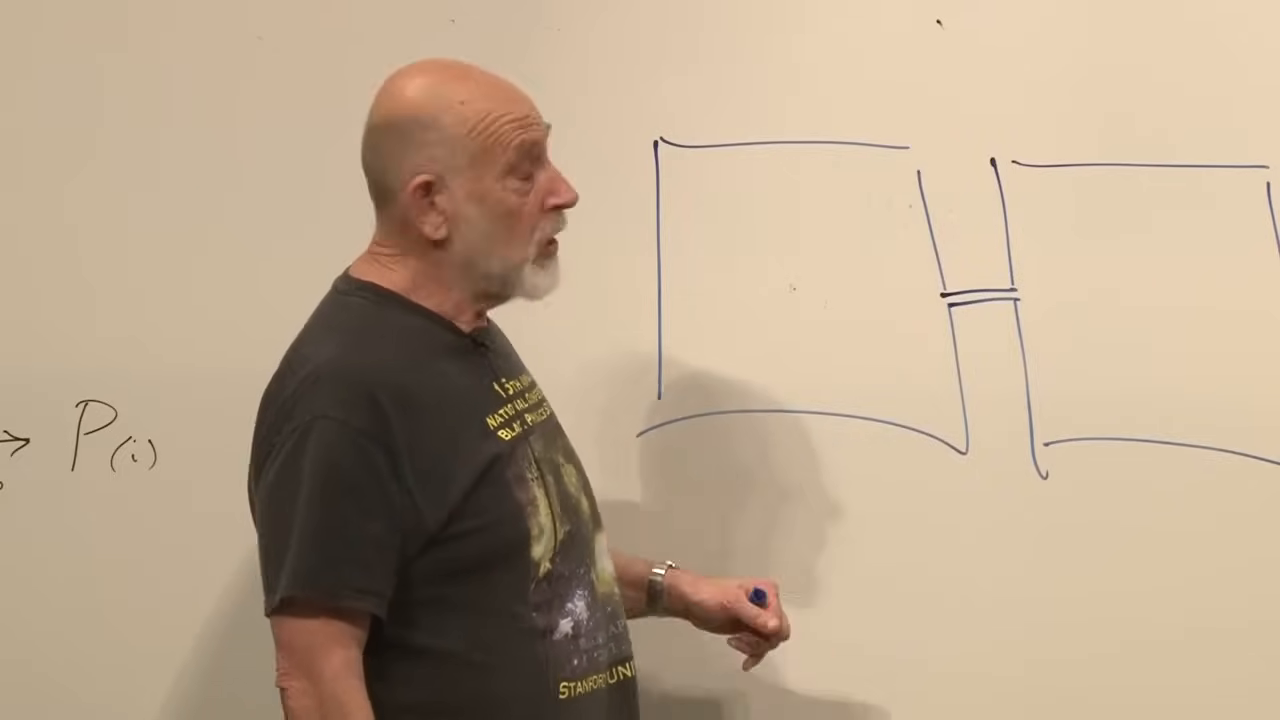
\includegraphics[width=0.92\textwidth]{lecture_01_figure_03.png}
\caption{兩個子系統由一條狹窄通道連接，能量可以經由通道流動。}
\lectureframe{00:39:19}
\end{figure}

\begin{figure}[htbp]
\centering
\begin{tikzpicture}[>=Latex]
\draw[thick,rounded corners=4pt] (-4,1.8) rectangle (-0.7,-1.5);
\draw[thick,rounded corners=4pt] (0.7,1.5) rectangle (4,-1.8);
\draw[thick] (-0.7,0.45) -- (0.7,0.45);
\draw[thick] (-0.7,-0.35) -- (0.7,-0.35);
\draw[<->,very thick] (-0.45,0.05) -- (0.45,0.05);
\node at (-2.35,0.15) {subsystem \(1\)};
\node at (2.35,-0.15) {subsystem \(2\)};
\node[above] at (0,0.5) {energy exchange};
\end{tikzpicture}
\caption{連接一旦打開，只有\(E_1+E_2\)守恆。能量如何分配便成為機率問題。}
\label{fig:sm1-connected-systems}
\end{figure}

給定總能量後，我們可以問：子系統\(1\)具有\(E_1\)、而子系統\(2\)具有其餘能量的機率是多少。相同的盒子，平均而言應具有相同能量，但平均值並不能描述完整的分佈。因此，要決定某個子系統的機率，一種方法是將它置於更大的封閉系統中，由該系統的守恆定律補足缺少的資訊。這種建構方式將在統計力學中反覆出現。

\section{好定律、壞定律與負第一定律}

並非每一種確定性更新規則都適合作為基本定律。考慮以下映射：
\begin{equation}
 \begin{aligned}
 R&\mapsto R,& B&\mapsto R,& Y&\mapsto R,\\
 G&\mapsto R,& O&\mapsto R,& P&\mapsto R.
 \end{aligned}
 \label{eq:sm1-all-to-red}
\end{equation}
它能完美預測未來：一步之後，狀態就是紅色。但它無法反向預測。一旦系統處於紅色，就無從得知它原先是藍色、黃色、綠色、橙色、紫色，還是紅色。

\begin{figure}[htbp]
\centering
\begin{tikzpicture}[
  >=Latex,
  state/.style={draw,circle,minimum size=8mm,inner sep=1pt}
]
\node[state,fill=red!12] (R) at (0,0) {$R$};
\node[state] (B) at (-3,1.6) {$B$};
\node[state] (Y) at (-3,0) {$Y$};
\node[state] (G) at (-3,-1.6) {$G$};
\node[state] (O) at (3,1.6) {$O$};
\node[state] (P) at (3,-1.6) {$P$};
\draw[->] (B) -- (R);
\draw[->] (Y) -- (R);
\draw[->] (G) -- (R);
\draw[->] (O) -- (R);
\draw[->] (P) -- (R);
\draw[->,loop above] (R) to (R);
\end{tikzpicture}
\caption{多對一的定律能預測下一個狀態，卻抹除了不同可能過去狀態之間的差異。}
\label{fig:sm1-bad-law}
\end{figure}

相較之下，閉合迴圈會保留這些差異。只要知道經過的時間，即使已過了數千個週期，我們仍能將狀態向前或向後演化。這條定律保留了不同初始條件之間的差異。Susskind 將這項要求稱為\emph{物理學的負第一定律}：資訊不會從根本上丟失。

對有限的離散狀態空間而言，圖示判準很簡單：
\begin{quote}
良好的定律中，每個狀態都恰好有一條向外箭頭，也恰好有一條指向它的箭頭。
\end{quote}
向外的箭頭決定未來；指向該狀態的箭頭則能重建過去。從數學上看，更新就是對狀態作置換。

\subsection{摩擦只是表面上的反例}

連續情形下的對應定理是劉維爾定理。摩擦看似與它矛盾。把橡皮擦在桌面上滑動，無論從哪裡開始，它最終都會停下來。示意性的阻力方程為
\begin{equation}
 m\ddot x=-\gamma\dot x,
 \qquad \gamma>0.
 \label{eq:sm1-drag}
\end{equation}
速度會按指數衰減。如果這就是密閉房間中每個粒子的根本定律，所有運動都會消失，溫度會降到零，而許多初始狀態會合併成同一個最終狀態。能量守恆會失效，資訊會消失，無序度也會降低。這就是一切狀態都變成紅色的連續版本。

真實的摩擦並非如此。橡皮擦會使桌面、橡皮擦本身和周遭環境升溫。微觀位置與動量會記錄可見運動中消失的那些差異。摩擦方程是省略未觀測自由度後，對子系統所用的有效方程；它不是描述完整封閉系統的基本耗散定律。

\begin{classroomqa}
\classquestion{微分方程
\(m\ddot x=-\gamma\dot x\)代表什麼？為什麼它不是描述封閉系統的基本定律？}
\lecturerresponse{它描述黏滯阻力。若只看這條方程，每個速度都會趨近於零，這會使氣體不論初始溫度如何，最後都冷卻到零。在完整的封閉系統描述中，流失的機械能和資訊會轉移到微觀自由度中。只有在略去這些變數之後，阻力方程才可靠。
\lecturetimestamp{00:44:40--00:48:56}}
\end{classroomqa}

\section{佔據狀態與最初的熵}

資訊守恆也可以用機率來表述。假設\(M\)個狀態中有\(N\)個被指定相同的機率，
\begin{equation}
 p_i=
 \begin{cases}
 1/M, & i\text{ in the occupied set},\\
 0, & i\text{ outside it}.
 \end{cases}
 \label{eq:sm1-uniform-occupied}
\end{equation}
保留資訊的更新可以重新排列哪些狀態被佔據，卻不能將它們合併。之後每個時刻，仍有\(M\)個狀態的機率為\(1/M\)。相較之下，壞映射\eqref{eq:sm1-all-to-red}可以將許多已佔據的狀態合併成一個。

數值\(M\)衡量無知程度。若\(M=N\)，每個狀態都有可能，我們的無知程度達到最大。若\(M=1\)，微觀狀態便已完全確知。因此，熵的第一個定義是
\begin{equation}
 S=\log M.
 \label{eq:sm1-entropy-logm}
\end{equation}
由此可得
\begin{equation}
 S_{\max}=\log N,
 \qquad
 S_{\min}=0.
\end{equation}
若狀態空間無限大，就不一定存在有限上限。

在這套論述中，熵先於溫度出現，甚至早於能量守恆的正式陳述。從這個意義上說，熵更為基本。然而，熵並非力學系統本身單獨具有的性質；它同時取決於系統，以及代表已知資訊的機率分佈。資訊不同的觀察者，可能會對同一力學系統指定不同的熵。

在精確的微觀演化下，已佔據的狀態只是重新排列，因此這個細粒化熵守恆。實際上，我們會失去時間資訊、捨棄關聯性，也無法追蹤數量龐大的變數。於是，機率分佈會擴散到更多可能性上，粗粒描述所指定的熵也隨之增加。即使方程沒有破壞資訊，我們能運用的描述仍可能失去資訊。

\begin{classroomqa}
\classquestion{具有\(N\)個狀態的有限系統，其可能的最大熵是多少？}
\lecturerresponse{最大熵為\(\log N\)，在所有\(N\)個狀態的機率都相等時達到。最小熵為零，在其中一個狀態的機率為一時達到。因此，熵衡量的不只是可用的狀態空間，也包括我們掌握資訊的情形。
\lecturetimestamp{00:56:46--00:58:19}}
\end{classroomqa}

\section{連續相空間中的劉維爾流}

對於位置與動量都是連續變數的粒子，微觀狀態是相空間中的一個點。我們以\(q_a\)表示座標，以\(p_a\)表示其共軛動量。粒子數目很多時，相空間會有極多個軸；二維圖上只有一個\(q\)和一個\(p\)，只是用來代替完整相空間的示意圖。相空間的維度必為偶數，因為每個座標都有一個相對應的動量。

假設用一個區域\(\Omega_0\)來表示我們掌握的資訊：機率密度在區域內均勻，區域外則為零。例如，知道每個粒子都在房間裡，就會限制位置座標；限制粒子的速率，則會限制動量座標。

哈密頓演化會使相空間中的每個點沿著軌跡運動。彼此相鄰的點仍會移動到相鄰的位置，而佔據區域則像不可壓縮流體的一團流體般演化：
\begin{figure}[htbp]
\centering
\begin{tikzpicture}[>=Latex,scale=0.95]
\draw[->] (-4.2,0) -- (4.3,0) node[right] {$q$};
\draw[->] (-3.7,-2.2) -- (-3.7,2.4) node[above] {$p$};
\draw[fill=blue!12,thick]
  (-3.0,-0.5) .. controls (-2.7,1.0) and (-1.3,1.2) .. (-0.9,0.1)
  .. controls (-0.6,-1.0) and (-2.2,-1.4) .. cycle;
\node at (-1.9,0.0) {$\Omega_0$};
\draw[->,very thick] (-0.3,0.2) -- (0.8,0.2);
\draw[fill=orange!15,thick]
  (1.2,-1.1) .. controls (1.5,0.3) and (2.3,1.8) .. (3.2,1.1)
  .. controls (3.6,0.7) and (2.8,-0.4) .. (2.5,-1.5)
  .. controls (2.1,-1.8) and (1.5,-1.6) .. cycle;
\node at (2.35,0.1) {$\Omega_t$};
\end{tikzpicture}
\caption{哈密頓流可以拉伸並剪切佔據的相空間區域，但會保持其體積不變。}
\label{fig:sm1-liouville-flow}
\end{figure}

劉維爾定理指出：
\begin{equation}
 \operatorname{Vol}(\Omega_t)
 =
 \operatorname{Vol}(\Omega_0).
 \label{eq:sm1-liouville-volume}
\end{equation}
若初始密度在\(\Omega_0\)上均勻，輸運後的密度就會在\(\Omega_t\)上均勻。這相當於在連續情形中，佔據狀態的數目與權重都保持不變。

這項定理也以幾何方式解開了摩擦之謎。若只看橡皮擦的可見動量，一團可能狀態似乎會朝\(p=0\)收縮。但在完整相空間中，這團狀態會擴散到橡皮擦和桌上分子的位置與動量等變數中。投影可以收縮，完整的高維體積卻仍保持不變。

\begin{classroomqa}
\classquestion{如果每條可見軌跡都趨近靜止，佔據的相空間區域是否已收縮到\(p=0\)軸上？}
\lecturerresponse{只有在約化後的投影中才是如此。完整系統還包含桌子、橡皮擦和周遭環境的微觀變數。可見的動量範圍縮小時，分佈會擴散到那些隱藏方向。劉維爾定理適用於完整的封閉相空間，而不是不完整的宏觀變數集合。
\lecturetimestamp{01:04:37--01:06:29}}
\end{classroomqa}

\section{從負第一定律到第一定律}

\subsection{簡談第零定律}

在陳述第一定律之前，先介紹第零定律很有幫助。熱平衡尚未定義，因此目前這條定律只是一項結構性陳述：
\begin{quote}
若系統\(A\)與\(B\)處於熱平衡，且\(B\)與\(C\)處於熱平衡，那麼\(A\)與\(C\)也處於熱平衡。
\end{quote}
這種遞移性日後會讓溫度得以定義。目前先暫且擱置。

\subsection{能量守恆}

封閉系統的第一定律就是
\begin{equation}
 \frac{dE}{dt}=0.
 \label{eq:sm1-first-law}
\end{equation}
這個簡潔的形式隱藏了它的力量。能量是一種守恆量，而「能量」一詞日後還會獲得更多熱力學上的意涵。

如果封閉系統由兩部分組成，而且兩部分的能量可以相加，
\begin{equation}
 E=E_1+E_2,
\end{equation}
那麼
\begin{equation}
 \frac{dE_1}{dt}+\frac{dE_2}{dt}=0,
 \qquad\text{or}\qquad
 \frac{dE_1}{dt}=-\frac{dE_2}{dt}.
 \label{eq:sm1-energy-exchange}
\end{equation}
第二種形式清楚表明能量如何交換：一個子系統失去的能量，會由另一個子系統獲得。

可加性假設需要審慎看待。兩個互相吸引的粒子各有動能，但它們的交互作用也會帶來一份屬於兩者整體的位能。總能量守恆，儘管它無法精確地寫成一個物體的能量加上另一個物體的能量。

熱力學往往可以採用極佳的可加近似，因為整體能量隨體積增加，而大型相鄰部分之間的短程交互作用能，主要隨接觸面積增加。把一張大桌子分成幾塊：每塊的內能取決於體積，而相鄰桌塊間的耦合則取決於接觸面。桌塊夠大時，後者相對較小。方程\eqref{eq:sm1-first-law}對整個封閉系統而言是精確的；子系統的形式\eqref{eq:sm1-energy-exchange}則假設交互作用能可以忽略。

\begin{classroomqa}
\audiencequestion{歸一化條件\(\sum_i p_i=1\)是否也假設列出的結果彼此互斥？}
\lecturerresponse{是的。狀態標籤的定義要求各種可能性彼此不重疊：骰子若處於黃色狀態，就不會同時處於紅色狀態。日常用語中顏色可以混合，但機率計算所採用的狀態劃分，必須由互斥的可能性構成。
\lecturetimestamp{01:12:14--01:12:55}}
\end{classroomqa}

\section{回到熵}

講課現在明確回到尚未處理完的問題。溫度雖然是感官熟悉的量，卻是推導而來的量。要明確定義溫度，必須先確立熵與能量的概念。

\subsection{一般機率分佈}

特殊定義\(S=\log M\)適用於\(M\)個狀態等機率、其他狀態的機率皆為零的情況。一般分佈不必是矩形的；各狀態標籤所對應的權重，可以平滑或不規則地變化。

\begin{figure}[htbp]
\centering
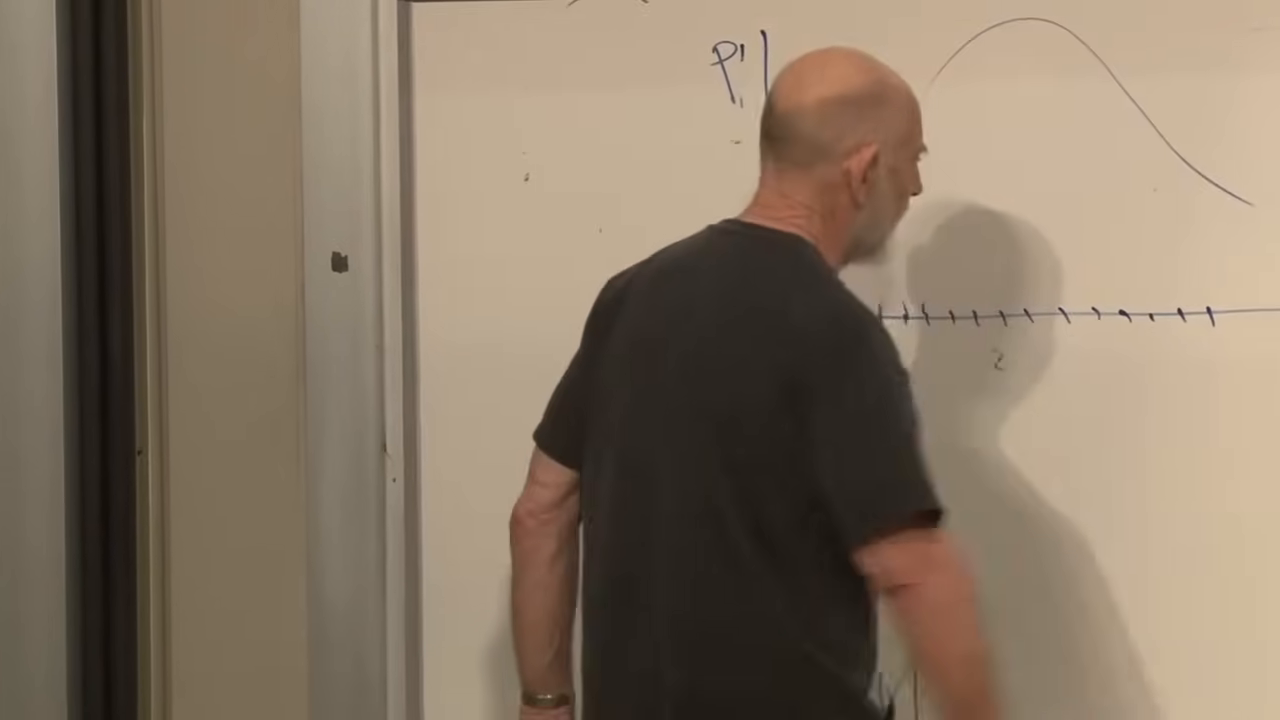
\includegraphics[width=0.92\textwidth]{lecture_01_figure_05.png}
\caption{繪於離散狀態標籤上的機率分佈。熵所需衡量的是分佈的展寬，而不是曲線的精確形狀。}
\lectureframe{01:14:40}
\end{figure}

\begin{figure}[htbp]
\centering
\resizebox{\linewidth}{!}{%
\begin{tikzpicture}[>=Latex,scale=0.93]
\draw[->] (-4.2,0) -- (4.4,0) node[right] {state label \(i\)};
\draw[->] (-4,0) -- (-4,3.2) node[above] {$p_i$};
\foreach \x in {-3.6,-3.1,...,3.6}
  \draw (\x,0.08) -- (\x,-0.08);
\draw[very thick]
  plot[smooth] coordinates {
  (-3.7,0.12) (-3.0,0.28) (-2.3,0.72) (-1.6,1.45)
  (-0.9,2.25) (-0.2,2.65) (0.5,2.28) (1.2,1.55)
  (1.9,0.88) (2.7,0.38) (3.5,0.14)};
\draw (-1.8,-0.18) -- (-1.8,-0.5);
\draw (1.8,-0.18) -- (1.8,-0.5);
\draw[<->] (-1.8,-0.46) -- (1.8,-0.46);
\node at (0,-0.82) {effective spread};
\end{tikzpicture}
}
\caption{窄分佈的不確定性小於寬分佈。熵必須衡量整個分佈。}
\label{fig:sm1-probability-spread}
\end{figure}

一般定義為
\begin{equation}
 S=-\sum_i p_i\log p_i.
 \label{eq:sm1-shannon-entropy}
\end{equation}
利用\eqref{eq:sm1-expectation}，可寫成
\begin{equation}
 S=-\langle\log p\rangle.
\end{equation}
負號是為了補償\(\log p_i<0\)（當\(0<p_i<1\)時）這一點。

\subsection{恢復均勻分佈的結果}

我們必須檢查一般公式是否能重現第一個定義。對於未佔據的狀態，\(p_i=0\)，而\(\log p_i\)會發散。兩者的乘積有明確的極限值
\begin{equation}
 \lim_{p\to0^+}p\log p=0.
 \label{eq:sm1-plogp-limit}
\end{equation}
因此，機率為零的狀態不會有任何貢獻。

\begin{classroomqa}
\audiencequestion{如果\(p_i=0\)，該項真的會消失嗎？零的對數是負無窮。}
\lecturerresponse{該項由極限\(\lim_{p\to0^+}p\log p\)定義，其值為零。因子\(p\)趨近於零的速度比對數發散的速度快。因此，機率任意小的狀態所作的貢獻也任意小，而機率恰為零的狀態則毫無貢獻。
\lecturetimestamp{01:18:27--01:19:46}}
\end{classroomqa}

對於\(M\)個佔據狀態中的每一個，都有\(p_i=1/M\)。因此
\begin{align}
 S
 &=-\sum_{\mathrm{occupied}\ i}
 \frac1M\log\!\left(\frac1M\right)\\
 &=-M\frac1M\log\!\left(\frac1M\right)\\
 &=-\log\!\left(\frac1M\right)
 =\log M.
 \label{eq:sm1-entropy-check}
\end{align}
一般表示式與特殊情況下的表示式完全一致。較寬廣的分佈會讓更多選項具有可觀的權重，因此熵較大；較集中的分佈則有較小的熵。

\begin{figure}[htbp]
\centering
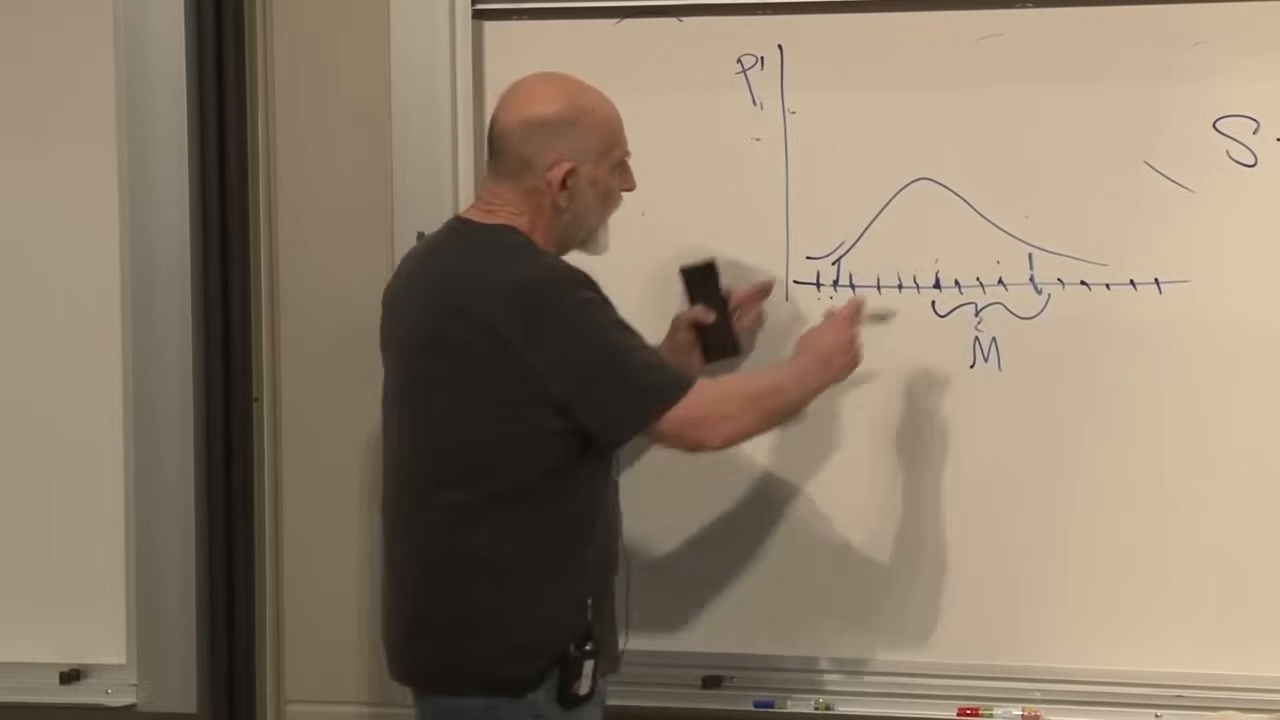
\includegraphics[width=0.92\textwidth]{lecture_01_figure_06.png}
\caption{圖中標示的寬度\(M\)突顯了顯著機率的分布範圍與熵之間的關聯。}
\lectureframe{01:16:42}
\end{figure}

熵屬於狀態空間上的機率分佈。它不是像單一微觀態的能量或動量那樣的單一可觀測量。精確狀態可以用集中在該狀態上的分佈表示，此時熵為零；但當我們掌握的資訊改變時，熵也會改變。

\section{硬幣、位元與明確計數}

令\(n\)為硬幣數目。微觀構型的數目為
\begin{equation}
 N=2^n.
 \label{eq:sm1-coin-state-count}
\end{equation}
如果我們對硬幣一無所知，所有\(2^n\)種構型的機率都相同，因此
\begin{equation}
 S_{\max}=\log(2^n)=n\log2.
 \label{eq:sm1-coin-max-entropy}
\end{equation}
熵會隨獨立硬幣的數目相加。

以\(2\)為底的對數下，完全未知的二態系統具有一位元的熵；以自然對數計算時，其熵為\(\log2\)。單位是約定俗成的；底層的排序與可加性不受影響。

在另一個極端，如果每枚硬幣的狀態都已知，就恰好只有一種構型的機率為一：
\begin{equation}
 S=0.
\end{equation}
掌握的資訊越多，熵就越小。

現在假設\(n\)枚硬幣中恰有一枚是反面，其餘都是正面，但反面的位置未知。共有\(n\)種等可能的構型，分別對應反面可能出現的位置，因此
\begin{equation}
 S=\log n.
 \label{eq:sm1-one-tail-entropy}
\end{equation}
這通常不是\(\log2\)的整數倍。位元是方便使用的單位，並不表示所有熵值都以整數位元為間隔。

\begin{classroomqa}
\audiencequestion{\(\log2\)的出現僅僅是因為每枚硬幣有兩種可能狀態嗎？如果一個元素有三種可能狀態，熵會是\(\log3\)嗎？}
\lecturerresponse{正是如此。一個有\(k\)種可能狀態、且各狀態均勻未知的元素，貢獻\(\log k\)。二元開關在電腦中特別方便，因為實體開關自然能實現兩種穩定狀態，而且二是最小的非平凡整數。
\lecturetimestamp{01:29:55--01:30:48}}
\end{classroomqa}

\begin{classroomqa}
\audiencequestion{對數的底數是什麼？}
\lecturerresponse{在這些物理公式中，\(\log\)表示自然對數。資訊理論學者常用底數\(2\)，因此熵直接以位元為單位。改變底數會讓所有熵值乘上一個固定的換算因子，但不會改變任何物理結論。
\lecturetimestamp{01:30:49--01:32:06}}
\end{classroomqa}

\section{連續相空間中的熵}

回到經典相空間\(\Gamma\)。如果機率密度在體積為\(V_\Gamma\)的區域內均勻分布，區域外則為零，那麼，這相當於計數\(M\)個等可能狀態：
\begin{equation}
 S=\log\!\left(\frac{V_\Gamma}{V_0}\right).
 \label{eq:sm1-continuous-uniform}
\end{equation}
這裡的\(V_\Gamma\)是座標與動量所構成的完整高維空間中的體積，不是一般的空間體積。固定體積\(V_0\)是參考相空間元，用來使對數的引數成為無因次量。令\(V_0=1\)，便得到黑板上使用的簡寫\(S=\log V_\Gamma\)。

對於一般的機率密度\(P(q,p)\)，離散求和會變成相空間積分。歸一化條件為
\begin{equation}
 \int_\Gamma d\Gamma\,P(q,p)=1,
 \label{eq:sm1-continuous-normalization}
\end{equation}
熵則為
\begin{equation}
 S=-\int_\Gamma d\Gamma\,
 P(q,p)\log\!\bigl[P(q,p)V_0\bigr].
 \label{eq:sm1-continuous-entropy}
\end{equation}
此密度表示每個相空間元中的機率。概念上，\eqref{eq:sm1-continuous-entropy}仍衡量機率分布得有多廣；若分布均勻於一個區域，其熵便化為佔據體積以參考相空間元為單位計算所得的對數。改變這個固定的參考元，會使所有連續熵值平移相同的加法常數，但熵差不變。

\begin{classroomqa}
\audiencequestion{為什麼座標符號從\(x\)改成了\(q\)？}
\lecturerresponse{物理上並沒有任何改變。經典力學常用\(x\)或\(q\)表示座標，並用\(p\)表示共軛動量。符號的更換只是筆誤；相空間的建構方式並未改變。
\lecturetimestamp{01:37:10--01:37:39}}
\end{classroomqa}

溫度與玻爾茲曼分佈刻意留待後續討論。接下來要先定義熱平衡，再找出對應的機率分佈。

\section{關於關聯、可加性與資訊的問題}

\subsection{關聯表示一次測量會改變另一個機率分佈}

對獨立硬幣一無所知時，每種構型的機率都相同。測量其中一枚硬幣，並不會讓我們得知任何其他硬幣的狀態；其他硬幣的機率分佈也不會改變。

單一反面硬幣的系綜則不同。如果測得其中一枚硬幣是反面，其他每枚就必定是正面。如果測得的是正面，唯一的反面必定位於其餘\(n-1\)枚硬幣之中，因此，其餘每個位置出現反面的條件機率為
\begin{equation}
\begin{aligned}
 p(&\text{tail at a specified remaining position}\\
   &\mid\text{measured head})=\frac{1}{n-1}.
\end{aligned}
 \label{eq:sm1-conditional-tail}
\end{equation}
這就是關聯：得知一個變數的狀態，會改變另一個變數所對應的機率分佈。

\begin{classroomqa}
\audiencequestion{熵的例子是否假設硬幣彼此獨立？}
\lecturerresponse{只有在以所有\(2^n\)種構型等機率來表示完全無知時，才是如此。在這種情況下，測量一枚硬幣不會改變其他硬幣的分佈。單一反面硬幣的例子則明確包含關聯：一次測量會更新我們對其他位置可能狀態的認知。所給定的資訊決定了採用哪一種機率分佈。
\lecturetimestamp{01:38:43--01:41:58}}
\end{classroomqa}

不連通軌道的例子在邏輯上也相同。測得守恆的\(+1\)或\(-1\)標籤，就會將所有後續狀態限制在其中一個扇區。以守恆量的資訊為條件，會改變容許的機率分佈。

對於彼此不相關的系統，熵具有可加性。若
\begin{equation}
 p_{ij}=p_i^{(A)}p_j^{(B)},
\end{equation}
則
\begin{align}
 S_{AB}
 &=-\sum_{i,j}p_i^{(A)}p_j^{(B)}
 \log\!\left[p_i^{(A)}p_j^{(B)}\right]\\
 &=S_A+S_B.
 \label{eq:sm1-entropy-additivity}
\end{align}
關聯會使這種因式分解不成立，並降低這對系統各自的不確定性總和。

作為練習，想像一排二元變數：若其中一個變數處於向上狀態，則它的每個鄰居處於向下狀態的機率都是四分之三。測量其中一個位置，會立即改變我們對鄰近位置的認知。這樣的分佈具有關聯；若不考慮這些關聯，就不能只把各位置單獨的熵相加來求得整體熵。

\subsection{玻爾茲曼、夏農與量子不確定性}

\begin{classroomqa}
\audiencequestion{早期熱力學中的熵與夏農資訊理論中的熵有何關係？}
\lecturerresponse{兩者都具有相同的函數形式：
\(-\sum_i p_i\log p_i\)。夏農通常使用底數為\(2\)的對數；物理學家則通常使用自然對數，並在以熱力學單位表示熵時乘回玻爾茲曼常數。數學上的差異只在於一個固定的換算因子，儘管兩者所依據的物理問題可能大不相同。
\lecturetimestamp{01:44:05--01:46:06}}
\end{classroomqa}

對於等機率的微觀態，熱力學公式常寫成
\begin{equation}
 S_{\mathrm{thermo}}=k_{\mathrm B}\log W,
 \label{eq:sm1-boltzmann-formula}
\end{equation}
其中\(W\)是可及微觀態的數目。在\(k_{\mathrm B}=1\)的單位制下，這正是\(S=\log W\)。玻爾茲曼常數負責在溫度單位與能量單位之間換算；溫度的自然微觀尺度就是能量。

\begin{classroomqa}
\audiencequestion{這種熵是否只是海森堡不確定性原理的另一種形式？}
\lecturerresponse{不是。這裡的熵衡量可能狀態上的機率分佈所具有的不確定性。用量子語言來說，它代表混合態的不確定性，而非純態也可能存在的內禀測量不確定性。必須將這兩種概念區分開來。
\lecturetimestamp{01:46:07--01:47:31}}
\end{classroomqa}

\section{目前已確立的內容}

我們的出發點並非定律本身具有隨機性。確定性動力學加上對初始狀態的不完全認識，就足以產生機率。單一軌道依據各狀態上停留的時間賦予權重；彼此不連通的軌道則揭示守恆量，也因此需要先指定各扇區之間的權重。容許的微觀定律會保留狀態間的區別；在有限狀態空間中，這表示每個狀態各有一條入箭頭與一條出箭頭；在連續力學中，則對應於劉維爾定理。

這種結構首先導出
\begin{equation}
 S=\log M
\end{equation}
其中\(M\)個佔據狀態的機率相同；接著導出
\begin{equation}
 S=-\sum_i p_i\log p_i,
\end{equation}
最後則得到相應的相空間積分。熵記錄的是一個機率分佈，因此也記錄了我們掌握資訊的狀態。即使實務上的粗粒化描述會遺漏細緻資訊，微觀定律仍保留這些資訊。

能量守恆提供了第一定律，而子系統能量具有可加性，則要求交互作用能可忽略。熵也在一項相應條件下具有可加性：子系統的機率分佈必須彼此不相關。這兩種可加性為下一步作準備；接下來將以熱平衡、溫度與玻爾茲曼分佈，建立能量與機率之間的關聯。
\chapter{由熵與能量定義溫度}

\lectureoverview{溫度最初是作為換算因子出現，用來將人類溫度計的讀值換算成微觀能量單位。將熱力學熵相應地換算為無量綱的統計熵後，我們以一族由單一參數標記的機率分布描述平衡態。導數\(dE/dS\)於是定義了溫度，而前兩條定律則說明，為何溫差會決定能量流動的方向。}

\section{換算因子與人類使用的單位}

物理學中的許多常數都是換算因子。光速可將距離換算成時間：
\begin{equation}
 t=\frac{x}{c}.
\end{equation}
如果距離和時間以相容的單位測量，就可以令\(c=1\)。這不會使任何物理效應消失；只是把兩種測量改用同一個尺度表示。

波茲曼常數具有相同的性質。它將人類尺度溫度計所測得的溫度換算成能量。「\emph{人類尺度}」這個形容詞很重要。選用這類單位，是因為宏觀儀器能夠產生並分辨相應的溫度，而不是因為微觀動力學特別偏好這些單位。

攝氏溫標是將標準壓力下水的冰點與沸點之間的溫差分成一百等分而定義的。開爾文的刻度間隔大小相同，但將零點定在絕對零度。若改用另一種物質、另一段溫差或華氏度，數值會改變，物理則不會改變。

\begin{classroomqa}
\audiencequestion{華氏溫標早在十七世紀就已經建立了嗎？}
\lecturerresponse{這裡不需要知道確切日期。重點是，這類溫標都是依據人們能夠製備和測量的溫度來設計的。每一度的大小是約定出來的，並非由微觀尺度決定。
\lecturetimestamp{00:01:34--00:01:50}}
\end{classroomqa}

這些溫標創立時，實驗尚無法探知熱的分子起源。宏觀溫度計可以測出一度的變化，卻無法測量單一分子的能量。因此，在人們尚未知道溫度從根本上是一種能量尺度之前，先訂出溫度單位是很自然的事。

\section{為什麼溫度的單位是能量}

考慮稀薄的單原子氣體。就此處的討論而言，稀薄表示可以忽略分子間的交互作用能。在熱平衡下，能量均分定理指出，每個平動二次自由度所分配到的能量為波茲曼常數乘以\(T_{\mathrm K}/2\)。在三維空間中，
\begin{equation}
 \left\langle E_{\mathrm{kin}}\right\rangle
 =\frac{3}{2}k_{\mathrm B}T_{\mathrm K}.
 \label{eq:sm2-equipartition-kelvin}
\end{equation}
因子三計算的是沿\(x\)、\(y\)和\(z\)方向的運動。二分之一因子則來自二次動能。

這個關係並非某一種分子所獨有。在平衡的氦與氧混合氣體中，每個可自由平動的粒子，其質心動能平均值都相同，儘管較重的粒子移動得較慢。由於
\begin{equation}
 E_{\mathrm{kin}}=\frac{1}{2}mv^2,
\end{equation}
特徵能量相同，就意味著\(v\propto m^{-1/2}\)。

這個想法還可以延伸到一個刻意極端的例子。將保齡球懸浮在流體中，並讓整個系統達到平衡。保齡球的布朗平動自由度，與分子遵循相同的能量尺度。球的速度極小，是因為它的質量極大；但溫度比較的是能量尺度，而非速度。

室溫下，\(T_{\mathrm K}\)約為\(300\,\mathrm K\)；相較之下，單一微觀自由度的能量以焦耳計極小。因此，換算因子也非常小：
\begin{equation}
 k_{\mathrm B}\simeq 1.38\times10^{-23}\,
 \mathrm{J\,K^{-1}}.
 \label{eq:sm2-boltzmann-value}
\end{equation}
這個尺度與亞佛加厥常數的關係並非巧合，而是彼此相連：
\begin{equation}
 R=N_{\mathrm A}k_{\mathrm B}.
\end{equation}
氣體常數\(R\)描述一莫耳粒子的尺度，而\(k_{\mathrm B}\)描述每個微觀組成粒子所對應的尺度。

基本公式中反覆出現\(k_{\mathrm B}T_{\mathrm K}\)這個組合。因此，定義
\begin{equation}
 T\equiv k_{\mathrm B}T_{\mathrm K}.
 \label{eq:sm2-energy-temperature}
\end{equation}
會更加簡潔。從現在起，\(T\)本身就以能量為單位，而
\eqref{eq:sm2-equipartition-kelvin}則變為
\begin{equation}
 \left\langle E_{\mathrm{kin}}\right\rangle=\frac{3}{2}T.
 \label{eq:sm2-equipartition-natural}
\end{equation}
若能量以焦耳為單位，溫度也就以焦耳為單位；若能量以電子伏特為單位，溫度也就以電子伏特為單位。自然界並沒有一種稱為「溫度單位」的新單位。

\section{熵的兩種慣例}

熵也有相應的換算。宏觀熱力學是從熱機分析發展而來。卡諾提出了關鍵的熱機推理；克勞修斯後來引入熱力學熵，並以\(S\)表示。在本書使用的記號中，我們將這個宏觀量記為\(S_{\mathrm C}\)。它的單位是能量除以溫度計所用的溫度單位，例如焦耳每開爾文。

統計熵是無量綱的。對離散分布而言，
\begin{equation}
 S=-\sum_i p_i\log p_i.
 \label{eq:sm2-statistical-entropy}
\end{equation}
使用自然對數時，公平二選一的熵為\(\log2\)；使用以二為底的對數時，相同的熵量稱為一位元。兩種熵的慣例之間有如下關係：
\begin{equation}
 S=\frac{S_{\mathrm C}}{k_{\mathrm B}},
 \qquad
 S_{\mathrm C}=k_{\mathrm B}S.
 \label{eq:sm2-entropy-conversion}
\end{equation}
宏觀量以\(\mathrm{J\,K^{-1}}\)為單位時，即使數值不大，也會對應到極大的無量綱熵，因為它計算的是分散在極大量微觀組成粒子中的資訊。

方程式\eqref{eq:sm2-energy-temperature}和
\eqref{eq:sm2-entropy-conversion}確立了全書採用的慣例：
\[
 [T]=[\text{energy}],
 \qquad
 [S]=1.
\]
在接下來的公式中，可以不寫出波茲曼常數；只要分別將\(T\)換成\(k_{\mathrm B}T_{\mathrm K}\)，並將\(S\)換成\(S_{\mathrm C}/k_{\mathrm B}\)，就能恢復它。

\begin{classroomqa}
\audiencequestion{除去因子\(3/2\)，新定義的溫度不就是以焦耳為單位的能量嗎？}
\lecturerresponse{如果選用焦耳作為能量單位，那麼確實如此。焦耳是MKS制中的\(\mathrm{kg\,m^2\,s^{-2}}\)單位。也可以改用電子伏特或其他能量單位；此時溫度就必須以相同的單位表示。因子\(3/2\)屬於理想氣體這個例子，並非溫度定義的一部分。
\lecturetimestamp{00:15:49--00:16:45}}
\end{classroomqa}

\begin{classroomqa}
\audiencequestion{如果黑板上指定的是開爾文，那麼\(k_{\mathrm B}\)不就是一個確定的常數嗎？}
\lecturerresponse{只有在溫度與能量所用的單位都指定之後，它的數值才確定。若將開爾文改成華氏度，或將焦耳改成電子伏特，數值就會改變。這正是換算因子隨單位而變的情形。
\lecturetimestamp{00:16:46--00:18:33}}
\end{classroomqa}

\begin{classroomqa}
\audiencequestion{波茲曼常數的數值是由實驗測定的嗎？}
\lecturerresponse{是的。歷史上，測定波茲曼常數需要原子及其數密度的微觀資訊。波茲曼早在這些量尚未被精確測定之前，就已理解分子能量與溫度的關係；這有如牛頓在重力常數尚未被精確測量之前，就已知道它所扮演的角色。
\lecturetimestamp{00:18:46--00:20:00}}
\end{classroomqa}

\section{平衡是一種統計狀態}

單位換算仍未定義溫度。觸摸高溫物體所帶來的感受，能提供有用的生物學直覺；但溫度是由能量和熵導出的物理量。

設想一個系統與一個宏觀條件固定的大環境接觸，能量可以在兩者之間傳遞。如果系統一開始的能量過多，平均而言就會失去能量；若能量不足，平均而言就會獲得能量。熱平衡時，微觀交換仍持續發生，但兩個方向都沒有淨平均能量流。

令\(i\)表示系統的一個精確微觀狀態，並以\(E_i\)表示該狀態的能量。平衡並不表示系統固定在某一個狀態。系統與環境的交互作用會不斷改變微觀狀態，因此我們為每種可能性指定一個機率\(P_i\)。基本關係如下：
\begin{align}
 \sum_i P_i &=1,
 \label{eq:sm2-normalization}\\
 \sum_i P_iE_i &=\overline E,
 \label{eq:sm2-mean-energy}\\
 S&=-\sum_iP_i\log P_i.
 \label{eq:sm2-equilibrium-entropy}
\end{align}
\(\overline E\)上方的橫線強調子系統的能量會發生漲落。一次測量可能得到某個值，下一次則可能得到另一個值；重複測量後，結果會符合某個分布，其平均值為\eqref{eq:sm2-mean-energy}。

\begin{figure}[t]
\centering
\includegraphics[width=0.82\textwidth]{lecture_02_figure_02.png}
\caption{黑板上的歸一化條件與平均能量：
\(\sum_iP(i)=1\)和\(\sum_iP(i)E(i)=\langle E\rangle\)。}
\lectureframe{00:24:10}
\end{figure}

\section{以平均能量標記的一族分布}

平衡分布會隨平均能量顯著改變。把一壺水放在爐子上，\(\overline E\)會上升；把它放進雪中，\(\overline E\)會下降。機率也會隨之改變。因此，平衡應視為一族由單一參數標記的分布，而非單一分布：
\begin{equation}
 P_i(\overline E).
 \label{eq:sm2-family}
\end{equation}
族中的每個分布都滿足
\begin{align}
 \sum_iP_i(\overline E)&=1,
 \label{eq:sm2-family-normalization}\\
 \sum_iP_i(\overline E)E_i&=\overline E.
 \label{eq:sm2-family-mean}
\end{align}

\begin{figure}[t]
\centering
\includegraphics[width=0.88\textwidth]{lecture_02_figure_03.png}
\caption{引入\(P(i,\overline E)\)。介紹這一族分布時，先前的歸一化、平均能量與熵方程式仍保留在黑板上。}
\lectureframe{00:26:29}
\end{figure}

在示意圖中，將狀態依\(E_i\)遞增排列。如此一來，橫軸既可讀作索引\(i\)，也可讀作相應的能量。平均能量較高時，機率權重會移向較右側的狀態。每條曲線的總面積都必須為一。

\begin{figure}[t]
\centering
\includegraphics[width=0.88\textwidth]{lecture_02_figure_04.png}
\caption{數個示意分布\(P(i,\overline E)\)。機率權重偏向右側的曲線，其平均能量較高；每條曲線仍各自歸一化。}
\lectureframe{00:28:40}
\end{figure}

\begin{figure}[t]
\centering
\begin{tikzpicture}[x=1cm,y=1cm]
\draw[->] (0,0) -- (7.4,0) node[right] {$E_i$};
\draw[->] (0,0) -- (0,3.25) node[above] {$P_i(\overline E)$};
\draw[thick,blue!70!black]
  plot[smooth] coordinates {(0,0) (0.35,1.6) (0.85,2.65) (1.45,1.45)
  (2.2,0.35) (3.0,0)};
\draw[thick,teal!70!black]
  plot[smooth] coordinates {(0,0) (0.7,0.7) (1.5,1.7) (2.5,2.0)
  (3.7,0.8) (4.8,0)};
\draw[thick,orange!80!black]
  plot[smooth] coordinates {(0,0) (1.3,0.3) (2.7,0.9) (4.3,1.45)
  (5.8,0.85) (7.0,0)};
\node[blue!70!black] at (1.0,2.95) {\(\overline E_1\)};
\node[teal!70!black] at (2.75,2.3) {\(\overline E_2\)};
\node[orange!80!black] at (5.2,1.7) {\(\overline E_3\)};
\node at (4.9,2.85) {\(\overline E_1<\overline E_2<\overline E_3\)};
\end{tikzpicture}
\caption{黑板草圖的清晰版本。曲線不必具有圖中這些精確形狀；這裡只用到歸一化條件，以及各曲線平均能量的大小順序。}
\end{figure}

\begin{classroomqa}
\audiencequestion{這個記號是否形成循環定義？平均能量是從分布計算而得，分布卻又以平均能量標記。}
\lecturerresponse{先從經驗上選定一族由單一參數標記的平衡分布。族中的每個分布都有一個平均能量。若不同分布的平均能量各不相同，就可以用平均能量作為標記這一族的參數。這個記號尚未推導出這一族分布；稍後將由波茲曼分布給出推導。
\lecturetimestamp{00:28:35--00:29:44}}
\end{classroomqa}

\begin{classroomqa}
\audiencequestion{為什麼說平均能量，而不說總能量？}
\lecturerresponse{子系統正與熱浴交換能量；例如，氣體容器的壁具有透熱性，因此周圍的大氣可作為熱浴。子系統的瞬時能量會漲落。多次測量會得到一個分布，而\(\overline E\)是這些測量結果的平均值。由子系統和熱浴組成的較大封閉系統，其能量仍可能固定。
\lecturetimestamp{00:29:46--00:30:56}}
\end{classroomqa}

\begin{classroomqa}
\audiencequestion{不同的微觀狀態能否具有相同的能量？不同的分布能否具有相同的平均能量？}
\lecturerresponse{兩者都有可能。只施加平均能量這項限制，仍容許許多種分布；因此，要選出這一特殊的單參數平衡分布族，還需要額外的物理論證。稍後會推導它的來源及其波茲曼形式。不同微觀狀態具有相同能量，則是另一個稱為簡併的問題。
\lecturetimestamp{00:30:58--00:32:22}}
\end{classroomqa}

\subsection{狀態標記、簡併與關聯}

有幾個容易混淆的概念，必須彼此區分。

第一，許多機率分布可能具有相同的平均能量。單靠平均能量限制，無法得出這一族由單一參數標記的平衡分布；它是系統達到平衡時所選出的特定分布族。稍後會將其形式辨認為波茲曼分布。

第二，不同的微觀狀態可能具有相同的能量，這稱為簡併。黑板上的討論暫時忽略能量完全相同的情形，使狀態能依能量明確排序。系統具有對稱性時，簡併其實很常見，但這不會造成概念上的困難：保留狀態標記\(i\)，允許\(E_i\)取相同值，並對所有狀態求和。

第三，關聯並非簡併的另一種說法。關聯涉及兩個隨機量的聯合分布，探討得知其中一個量後，另一個量的機率是否會改變。在同一份微觀狀態列表中，互斥的標記\(i\)和\(j\)本身並不是正在計算關聯的兩個隨機變數。

\begin{classroomqa}
\audiencequestion{這個推導是否假設不同的\(i\)態彼此獨立？如果其中兩個態彼此相關，該怎麼辦？}
\lecturerresponse{狀態標記是單一微觀隨機變數的一個可能取值。獨立性與關聯性需要兩個具有聯合分布的變數，因此這些術語不能直接用來描述此列表中的兩個替代標記。不同狀態具有相同能量，則是簡併問題。
\lecturetimestamp{00:32:23--00:33:22}}
\end{classroomqa}

\begin{classroomqa}
\audiencequestion{如果兩個不同狀態的能量完全相同，該怎麼辦？}
\lecturerresponse{這就是簡併。為了繪製目前的圖，我們採用一項簡化假設：任意兩個狀態的能量都不相同，並依能量遞增排列。後面的機率公式不需要這項假設；簡併的狀態只要分別計數即可。
\lecturetimestamp{00:33:23--00:34:04}}
\end{classroomqa}

\begin{classroomqa}
\audiencequestion{索引\(i\)的意義是任意的嗎？}
\lecturerresponse{微觀狀態本身並非任意：每個狀態都指定了精確描述系統所需的所有位置、動量或其他資料。任意的是狀態的名稱，因此在圖中我們選擇依能量遞增的順序標記狀態。
\lecturetimestamp{00:34:06--00:35:15}}
\end{classroomqa}

\section{熵成為能量的函數}

平衡分布族中的每個成員都有熵。將\eqref{eq:sm2-family}代入\eqref{eq:sm2-equilibrium-entropy}，得到
\begin{equation}
 S(\overline E)
 =-\sum_iP_i(\overline E)\log P_i(\overline E).
 \label{eq:sm2-entropy-energy}
\end{equation}
這不是所有物理系統共用的普適函數；它取決於系統的能譜和平衡分布族。不過，一旦指定了這一族，能量與熵便相互關聯：沿著這一族改變分布時，兩者都會改變。

一般而言，隨著平均能量上升，系統會把機率分散到更多狀態，因此\(S\)通常會隨\(\overline E\)增加。目前先假設兩者的關係是光滑且局部可逆的。雖然例外情形也很重要，但先看簡單情況，就能引出所需的定義。

\section{定義溫度的導數}

問一個具體的問題：若要讓熵增加一個二元選擇的熵量，平均能量需要改變多少？以自然對數為單位，這個熵增量是\(\log2\)。

對於光滑分布族中彼此相鄰的成員，
\begin{equation}
 dE=\frac{dE}{dS}\,dS.
 \label{eq:sm2-differential-identity}
\end{equation}
此時，這個方程式不過是鏈鎖律。然而，它的係數恰好具有溫度所需的量綱與物理作用。

\begin{definition}
以能量為單位的溫度定義為
\begin{equation}
 T\equiv\frac{dE}{dS}.
 \label{eq:sm2-temperature-definition}
\end{equation}
等價地，
\begin{equation}
 dE=T\,dS,
 \qquad
 dS=\frac{1}{T}\,dE.
 \label{eq:sm2-fundamental-differentials}
\end{equation}
\end{definition}

對於一個位元所對應的微小變化，
\begin{equation}
 \Delta E\simeq T\log2.
 \label{eq:sm2-one-bit-energy}
\end{equation}
特別考慮一個位元，只是為了讓導數的意義更具體。任何微小的熵變都遵循相同的局部關係。

\begin{classroomqa}
\audiencequestion{既然熵寫成\(S(E)\)，那麼\(dS/dE\)不是更自然的導數嗎？}
\lecturerresponse{只要兩者的關係在局部可逆，這兩個導數就包含相同資訊：
\[
 \frac{dE}{dS}=\left(\frac{dS}{dE}\right)^{-1}.
\]
依慣例，溫度定義為\(dE/dS\)，而逆溫度則為\(dS/dE=1/T\)。
\lecturetimestamp{00:40:24--00:40:54}}
\end{classroomqa}

這裡只有一個熱力學變數在變化，因此用普通導數就足夠了。若體積、粒子數、磁化強度或其他變數也可變化，就必須使用偏導數，並說明哪些量維持不變。目前的定義是更一般的熱力學幾何中，僅有一個變數變化的情形。

\subsection{為什麼波茲曼常數會消去}

再簡短回顧溫度計所用的單位。利用
\[
 T=k_{\mathrm B}T_{\mathrm K},
 \qquad
 S=\frac{S_{\mathrm C}}{k_{\mathrm B}},
\]
基本關係變為
\begin{align}
 dE
 &=\bigl(k_{\mathrm B}T_{\mathrm K}\bigr)
   d\left(\frac{S_{\mathrm C}}{k_{\mathrm B}}\right)\\
 &=T_{\mathrm K}\,dS_{\mathrm C}.
 \label{eq:sm2-carnot-form}
\end{align}
溫度中含有一個\(k_{\mathrm B}\)因子，熵中則含有它的倒數，兩者正好抵消。這就是為什麼傳統熱力學教材可以不寫出波茲曼常數，直接寫成\eqref{eq:sm2-carnot-form}。

\begin{classroomqa}
\audiencequestion{\(S(E)\)必須可逆嗎？}
\lecturerresponse{不一定。在此處考慮的一般系統中，增加能量通常會使平衡分布變得更廣，並使熵增加，因此\(S(E)\)是單調函數，而且\(T>0\)。能譜有上限的系統可能是反例；其中有些區域的熵會隨能量增加而減少，統計溫度也會是負值。目前先不討論這些情形。
\lecturetimestamp{00:44:30--00:45:57}}
\end{classroomqa}

\section{從抽象導數到熱與冷}

以導數定義溫度雖然普適，仍然相當抽象。我們希望重新得到熟悉的說法：能量會從較熱的物體流向較冷的物體。觸摸高溫表面所感到的疼痛屬於生物學範疇；顏色與物體發出的輻射則取決於光的性質。即使忽略輻射，統計定義也應適用於理想化的氣體。

\begin{classroomqa}
\audiencequestion{高溫物體發出的光，能否作為溫度的基本定義？}
\lecturerresponse{輻射可用來測溫，但這會牽涉光的物理學。統計力學必須能為一盒氣體這類系統定義溫度，而不依賴光學性質。能量交換的方向才是更普遍的判準。
\lecturetimestamp{00:46:42--00:47:20}}
\end{classroomqa}

準備兩個系統\(A\)和\(B\)，讓它們各自先處於平衡態，溫度分別為\(T_A\)和\(T_B\)。起初兩者彼此隔離，接著透過微弱的熱接觸將它們連接起來：這條\emph{細管}允許少量能量來回傳遞，同時不破壞任一子系統的獨立性。

\begin{figure}[t]
\centering
\includegraphics[width=0.88\textwidth]{lecture_02_figure_05.png}
\caption{分別準備好的系統\(A\)和\(B\)，其溫度分別標記為\(T_A\)和\(T_B\)；圖示為考慮微弱熱接觸之前的情形。}
\lectureframe{00:48:55}
\end{figure}

\begin{figure}[t]
\centering
\begin{tikzpicture}[>=Stealth]
\draw[rounded corners,thick,fill=blue!6] (0,0) rectangle (2.6,2.4);
\draw[rounded corners,thick,fill=orange!8] (5.4,0) rectangle (8,2.4);
\draw[thick] (2.6,1.35) -- (5.4,1.35);
\draw[thick] (2.6,1.05) -- (5.4,1.05);
\draw[<->,very thick] (3.15,1.2) -- (4.85,1.2)
  node[midway,above] {\(\delta E\)};
\node at (1.3,1.45) {\Large \(A\)};
\node at (6.7,1.45) {\Large \(B\)};
\node at (1.3,0.65) {\(T_A,S_A,E_A\)};
\node at (6.7,0.65) {\(T_B,S_B,E_B\)};
\node at (4,0.35) {\small weak thermal contact};
\end{tikzpicture}
\caption{能量透過微弱接觸而漲落，同時整個組合系統維持孤立。}
\end{figure}

不失一般性，假設
\begin{equation}
 T_B>T_A.
 \label{eq:sm2-temperature-order}
\end{equation}
根據經驗，\(B\)應會失去能量，而\(A\)應會獲得能量。三項事實可以將這個預期轉化為計算。

\subsection{熵的可加性}

對於兩個微弱耦合的子系統，若兩者的微觀可能性彼此獨立，組合後的可能狀態數便是兩者狀態數的乘積：
\[
 W_{AB}=W_AW_B.
\]
熵是狀態數的對數，因此
\begin{equation}
 S_{\mathrm{tot}}=S_A+S_B.
 \label{eq:sm2-entropy-additivity}
\end{equation}
直接計算乘積分布的夏農熵，也會得到相同結果。

\begin{classroomqa}
\classquestion{為什麼組合系統的熵會相加？}
\lecturerresponse{因為底層可能狀態的數目會相乘，而熵取的是對數：
\(\log(W_AW_B)=\log W_A+\log W_B\)。交互作用微弱，才能將系統描述為兩個子系統，也才能得到這個主要的可加形式。
\lecturetimestamp{00:51:06--00:52:03}}
\end{classroomqa}

\subsection{第一定律與第二定律}

組合系統是孤立的，因此內部交換的能量守恆：
\begin{equation}
 dE_A+dE_B=0,
 \qquad
 dE_B=-dE_A.
 \label{eq:sm2-first-law}
\end{equation}
這就是本例中的第一定律。

此處先將第二定律視為一項公設；稍後會進一步說明其更深層的原因。相連的兩個系統逐漸弛豫到新的平衡態時，
\begin{equation}
 dS_{\mathrm{tot}}=dS_A+dS_B\geq0.
 \label{eq:sm2-second-law}
\end{equation}
嚴格不等式描述系統自發地向平衡態弛豫；在平衡態下，對可逆的一階變化，等號成立。

最後，溫度的定義適用於每個子系統：
\begin{equation}
 dE_A=T_A\,dS_A,
 \qquad
 dE_B=T_B\,dS_B.
 \label{eq:sm2-two-temperatures}
\end{equation}

\begin{figure}[H]
\centering
\includegraphics[width=0.88\textwidth]{lecture_02_figure_06.png}
\caption{黑板推導結尾的兩個子系統關係式：
\(dE_A=T_A\,dS_A\)和\(dE_B=T_B\,dS_B\)。}
\lectureframe{00:54:00}
\end{figure}

\subsection{能量流動的方向}

這些方程式已足以確定淨能量傳遞的方向。將
\(dS_A=dE_A/T_A\)、\(dS_B=dE_B/T_B\)和
\eqref{eq:sm2-first-law}代入\eqref{eq:sm2-second-law}：
\begin{align}
 dS_{\mathrm{tot}}
 &=\frac{dE_A}{T_A}+\frac{dE_B}{T_B}\\
 &=dE_A\left(\frac{1}{T_A}-\frac{1}{T_B}\right)\geq0.
 \label{eq:sm2-flow-sign}
\end{align}
若\(T_B>T_A>0\)，則
\[
 \frac{1}{T_A}-\frac{1}{T_B}>0.
\]
因此，方程式\eqref{eq:sm2-flow-sign}要求
\[
 dE_A>0,
 \qquad
 dE_B<0.
\]
較冷的系統\(A\)會獲得能量，較熱的系統\(B\)則會失去能量。當\(T_A=T_B\)時，一階熵變不偏好任何方向，微觀交換彼此平衡，淨能量流為零。因此，抽象導數\(T=dE/dS\)確實重現了熱與冷在操作上的區別。
\chapter{多重度、熵與受限平衡}

\lectureoverview{一旦機率分布中的各個狀態具有能量，這個分布便成為熱力學對象。我們先把熵增加與平衡化連結起來，並利用\(dE=T\,dS\)推導熱流的方向。接著，我們以大量複本取代單一系統，計算每組佔據數所對應的排列數，並證明這個多重度的對數等於熵乘以\(N\)。因此，平衡問題就是在約束條件下求熵的最大值；拉格朗日乘數則提供求解所需的方法。}

\section{三個基本量}

令\(i\)標記系統可用的離散狀態。目前採用離散狀態很方便，因為我們可以直接計數，而不必引入相空間測度。若狀態\(i\)的機率為\(P_i\)，則\begin{equation}
 \sum_i P_i=1.
 \label{eq:sm3-normalization}
\end{equation}若該狀態的能量為\(E_i\)，平均能量為\begin{equation}
 \overline E=\sum_iP_iE_i.
 \label{eq:sm3-mean-energy}
\end{equation}\emph{平均}一詞很重要。系統在任何單一微觀態中都不必具有\(\overline E\)這個值；它是各種可能值依機率加權所得的平均。

\begin{classroomqa}\classquestion{這裡的機率與統計之間，是否有值得區分之處？}\lecturerresponse{機率為可能結果提供模型；統計通常則從觀測資料出發，探問能據此推論什麼。本計算使用機率分布，不過同樣的平均值也自然會出現在統計資料中。課堂上的這段非正式問答對兩個詞的用法較為寬鬆，因為這項區別不影響接下來的物理內容。\lecturetimestamp{00:01:39--00:02:21}}\end{classroomqa}

分布的熵為\begin{equation}
 S[P]=-\sum_iP_i\log P_i.
 \label{eq:sm3-entropy}
\end{equation}此式非負。每個非零機率都滿足\(0<P_i\leq1\)，因此\(\log P_i\leq0\)；當\(P_i\to0\)時，則採用通常的極限值\(P_i\log P_i\to0\)。

\begin{figure}[t]\centering
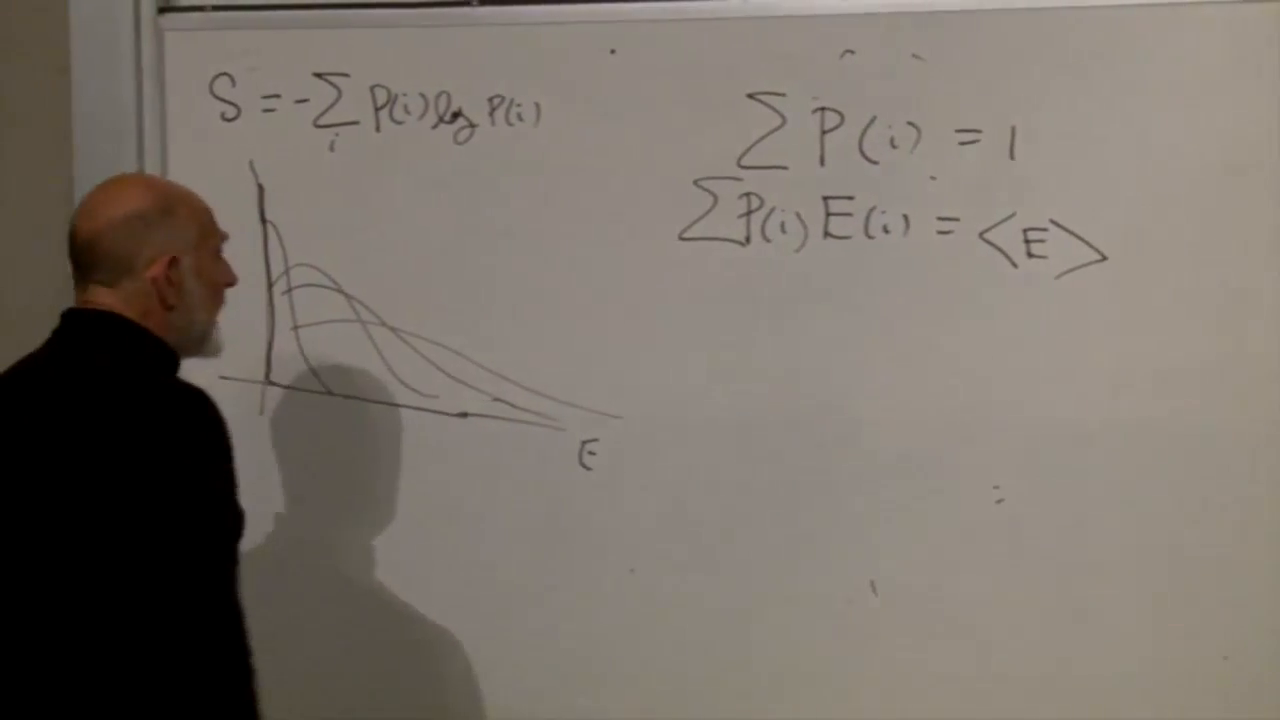
\includegraphics[width=0.88\textwidth]{lecture_03_figure_02.png}\caption{開場板書將熵、歸一化與平均能量的公式，以及一系列定性描繪的平衡分布，一併列出。}\lectureframe{00:06:44}\end{figure}

\section{作為一族分布的平衡}

上一講留下了一族由單一參數標記的平衡分布。雖然可以用溫度標記這一族分布，但目前用平均能量\(\overline E\)來標記更為方便。在可能的最低能量下，分布集中於基態：\[
 P_i=\delta_{i0}.
\]此時我們對系統所處的狀態毫無不確定性，且\(S=0\)。平衡分布涵蓋的能階愈多，其平均能量與熵也都愈大。

這個敘述只適用於熱平衡分布這一族，並非適用於任意構造的分布族。任意一族分布可能在趨向較高能量的同時變得更窄。接下來要推導的平衡分布，在通常的正溫度範圍內不會如此。沿著這一族分布，\begin{equation}
 \frac{dS}{d\overline E}>0.
 \label{eq:sm3-positive-temperature-branch}
\end{equation}具有有界能譜的系統也可能有導數為負的分支。這些負溫度區域確實存在，但本段論證暫且不予討論。

熱平衡不代表微觀上靜止。分子仍持續運動、碰撞並交換能量。達到定常的是宏觀描述：分布不再呈現淨漂移，系統中彼此分隔的部分之間也不再有淨能量流。

\section{以統計語言表述熱力學定律}

第一定律是能量守恆。第二定律指出，孤立宏觀系統的熱力學熵不會減少：\begin{equation}
 \Delta S_{\mathrm{tot}}\geq0.
 \label{eq:sm3-second-law}
\end{equation}等號表示系統處於平衡或經歷理想可逆變化；自發弛豫通常會使熵嚴格增加。

以機率描述時，弛豫會使權重分散到我們仍加以區分的各種宏觀可能性上。這項敘述有一個講座中特別強調的限定：我們正在進行\emph{粗粒化}。精確的哈密頓演化會保留細粒化的相空間熵。宏觀熵之所以增加，是因為我們不再追蹤微觀關聯與細節。這些資訊的流失會使約化描述更為分散。反之，若分布自發變窄，就表示我們在未進行測量的情況下取得了微觀資訊。

第零定律指出，系統能達到熱平衡，而且平衡具有傳遞性。若\(A\)與\(B\)處於平衡，且\(B\)與\(C\)處於平衡，那麼\(A\)便與\(C\)處於平衡。溫度提供一個數值，讓這種傳遞關係一目了然：\[
 T_A=T_B,\qquad T_B=T_C
 \quad\Longrightarrow\quad
 T_A=T_C.
\]在非平衡狀態下，能量會由溫度較高的子系統流向溫度較低的子系統。溫度相同時，淨能量流便停止。現在我們要從溫度的熵定義推導這項操作性敘述。

\section{為何能量會由熱端流向冷端}

考慮兩個弱耦合子系統\(A\)與\(B\)。兩者各自都已達到內部平衡，但溫度不同。選取標記，使得\begin{equation}
 T_B>T_A>0.
 \label{eq:sm3-temperature-order}
\end{equation}在微小的能量交換過程中，總能量守恆給出\begin{equation}
 dE_A+dE_B=0.
 \label{eq:sm3-energy-conservation}
\end{equation}第二定律則給出\begin{equation}
 dS_A+dS_B\geq0.
 \label{eq:sm3-entropy-change}
\end{equation}對每個已達內部平衡的子系統，溫度定義為\begin{equation}
 dE_X=T_X\,dS_X,
 \qquad X=A,B.
 \label{eq:sm3-temperature-differential}
\end{equation}將這個關係代入\eqref{eq:sm3-energy-conservation}，得到\begin{equation}
 T_A\,dS_A+T_B\,dS_B=0,
\end{equation}因此\begin{equation}
 dS_B=-\frac{T_A}{T_B}\,dS_A.
 \label{eq:sm3-dsb}
\end{equation}再將此結果代入\eqref{eq:sm3-entropy-change}：\begin{align}
 dS_{\mathrm{tot}}
 &=dS_A-\frac{T_A}{T_B}dS_A\\
 &=\frac{T_B-T_A}{T_B}\,dS_A\geq0.
 \label{eq:sm3-flow-entropy}
\end{align}由於\(T_B-T_A>0\)且\(T_B>0\)，自發交換必須滿足\[
 dS_A>0.
\]於是，方程式\eqref{eq:sm3-temperature-differential}給出\begin{equation}
 dE_A=T_A\,dS_A>0,
 \qquad
 dE_B=-dE_A<0.
 \label{eq:sm3-hot-to-cold}
\end{equation}能量已由較熱的子系統\(B\)流向較冷的子系統\(A\)。此處的熱，就是傳遞中的能量。能量流會持續到\(T_A=T_B\)為止；此時一階熵變不再偏向任何一個方向。

同一結果也可以用一行表示：\begin{equation}
 dS_{\mathrm{tot}}
 =dE_A\left(\frac{1}{T_A}-\frac{1}{T_B}\right)\geq0.
 \label{eq:sm3-compact-flow}
\end{equation}逆溫度差的正負決定\(dE_A\)的正負。之後在討論正則系綜時，這種簡潔的形式會很自然地派上用場。

\begin{classroomqa}\audiencequestion{這個論證是否假設\(A\)與\(B\)都已經達到內部平衡？}\lecturerresponse{是。指定單一的\(T_A\)或\(T_B\)，就已經作出這項假設。若某個子系統尚未達到內部平衡，就把它分成更小的區域，並在能夠定義溫度的區域逐一套用這個論證。整體弛豫便由各區域之間的能量交換所構成。\lecturetimestamp{00:24:38--00:25:22}}\end{classroomqa}

\section{什麼才算是一個態？}

在討論平衡機率之前，我們必須先弄清楚標記\(i\)代表什麼。微觀態是物理定律所允許、對系統最完整的描述。在經典力學中，可以把它想成所有粒子的位置與動量。在量子力學中，態則是完整的量子態；不確定性原理使我們無法同時精確指定每個粒子的經典位置與動量。

對於有限盒中的量子系統，相關的態數可以是離散的。在適當的極限下，密集量子態的總和會轉化為相空間積分，經典統計力學也由此導出。這個取極限的過程還會引入相空間元，用以使連續情形下的熵成為無量綱量；這並非只要把求和符號換成積分符號就能做到。

\begin{classroomqa}\audiencequestion{對氣體而言，是否可以把一個態想成每個分子的位置與動量？}\lecturerresponse{這是正確的經典圖像。更一般地說，態代表在物理定律限制下，原則上能夠知道的系統資訊。量子力學改變了這種完整描述的形式，也使有限體積下的計數成為離散的。從量子總和回到經典積分，需要真正進行取極限的推導，並非一行代換就能完成。\lecturetimestamp{00:25:31--00:27:38}}\end{classroomqa}

\section{由複本構成的熱浴}

現在有個棘手的問題無法迴避：系統達到平衡後，什麼決定了\(P_i\)？

讓子系統與一個極大的熱浴接觸。能量可以來回交換，但熱浴的自由度非常多，因此少量能量的轉移幾乎不會改變它的溫度。一種特別方便的熱浴，是由許多彼此弱耦合的子系統複本構成。其中一個複本是我們研究的系統，其餘複本則構成它的環境。

這種構造常可模擬真實的宏觀系統。把一個大致均勻的大型物體分成許多相似的區塊；每個區塊都是一個子系統，其餘區塊則充當它的熱浴。令\(N\)表示複本總數。課堂示範用了九個複本與三種以顏色區分的態標記，但計數結果並不取決於這些特定數字。

令\(n_i\)表示處於態\(i\)的複本數目。這些數目稱為\emph{佔據數}。可能的能階或許有無限多個，但在總能量有限時，大部分極高能階的佔據數都可以忽略或為零。

第一個約束條件只涉及複本總數：\begin{equation}
 \sum_i n_i=N.
 \label{eq:sm3-number-constraint}
\end{equation}第二個約束條件是總能量：\begin{equation}
 \sum_i n_iE_i=N\overline E.
 \label{eq:sm3-total-energy-constraint}
\end{equation}等式右側是廣延量。若複本數加倍，而統計狀態保持不變，總能量便加倍，但每個複本的平均能量仍為\(\overline E\)。

\begin{classroomqa}\audiencequestion{複本構造是否也必須滿足能量約束？}\lecturerresponse{是。佔據數總和必須等於\(N\)，而各佔據數乘上對應能量後的總和，必須等於固定總能量\(N\overline E\)。這正是接下來限制熵最大化問題的兩項約束。\lecturetimestamp{00:37:12--00:39:54}}\end{classroomqa}

隨機選取一個複本，它處於態\(i\)的機率就是該態所占的比例：\begin{equation}
 P_i=\frac{n_i}{N},
 \qquad
 n_i=NP_i.
 \label{eq:sm3-frequency-probability}
\end{equation}

\begin{figure}[t]\centering
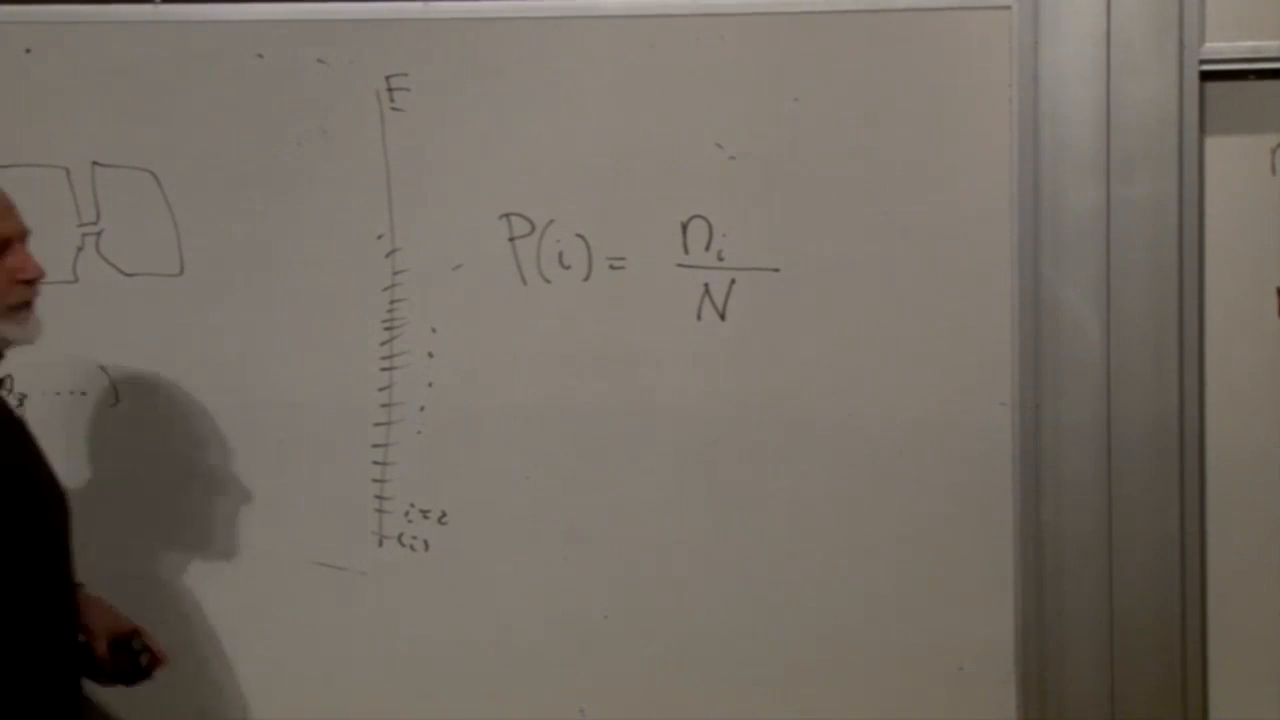
\includegraphics[width=0.82\textwidth]{lecture_03_figure_03.png}\caption{能階圖，以及將機率視為佔據比例\(P_i=n_i/N\)。}\lectureframe{00:41:40}\end{figure}

\begin{classroomqa}\audiencequestion{黑板上的記號\(N(i)\)是否有別於\(n_i\)？}\lecturerresponse{沒有。兩者都表示態\(i\)的佔據數。我們統一使用\(n_i\)，並以大寫\(N\)表示複本總數。\lecturetimestamp{00:41:28--00:41:33}}\end{classroomqa}

將\eqref{eq:sm3-number-constraint}與\eqref{eq:sm3-total-energy-constraint}除以\(N\)，便可還原為機率約束：\begin{equation}
 \sum_iP_i=1,
 \qquad
 \sum_iP_iE_i=\overline E.
 \label{eq:sm3-probability-constraints}
\end{equation}因此，以系綜頻率解釋機率，便重新得到一開始列出的方程式。

\section{佔據模式的多重度}

固定一組佔據數\(\{n_i\}\)。將\(N\)個可區分的複本分配到各個態，有多少種分配方式能恰好實現這組佔據數？答案是多項式係數：\begin{equation}
 C(\{n_i\})=\frac{N!}{\prod_i n_i!}.
 \label{eq:sm3-multiplicity}
\end{equation}來看分母的由來：先將全部\(N\)個帶有標記的複本排成\(N!\)種次序。處於同一態的\(n_i\)個複本彼此交換，不會形成新的佔據分配，因此每個態都要除以\(n_i!\)。

\begin{figure}[t]\centering
\includegraphics[width=0.88\textwidth]{lecture_03_figure_04.png}\caption{黑板上寫出的多項式多重度\(C=N!/\prod_i n_i!\)。}\lectureframe{00:46:55}\end{figure}

未佔據的能階不會造成問題，因為\(0!=1\)。若所有複本都處於同一態，則\[
 C=\frac{N!}{N!}=1,
\]結果如預期。若三個複本分別處於三個指定的不同態，則\[
 C=\frac{3!}{1!\,1!\,1!}=6.
\]若兩個複本分別處於兩個指定的態，公式給出兩種分配方式：交換兩個帶標記的複本所處的態。

\begin{classroomqa}\audiencequestion{是否可能有多組佔據數都滿足這兩項約束？}\lecturerresponse{通常有很多組。方程式\eqref{eq:sm3-multiplicity}先計算某一組固定佔據數\(\{n_i\}\)所對應的排列數，尚未判斷這組佔據數是否符合約束。下一步才是比較所有符合約束的組合，找出多重度最大的那一組。\lecturetimestamp{00:48:07--00:48:43}}\end{classroomqa}

統計假設是：對孤立系統而言，所有相容的微觀分配一視同仁。因此，能由較多分配方式實現的宏觀佔據模式，出現的機率也較高。當\(N\)很大時，分數\(n_i/N\)的分布會高度集中。平衡分數就是在滿足\eqref{eq:sm3-number-constraint}與\eqref{eq:sm3-total-energy-constraint}的條件下，使\(C\)最大的那些值。

\section{斯特林近似}

在\(N\)達到宏觀尺度之前，階乘就已經大得驚人，因此我們改用階乘的對數。先從\begin{equation}
 \log N!=\sum_{x=1}^{N}\log x.
 \label{eq:sm3-log-factorial-sum}
\end{equation}開始。當\(N\)很大時，這個總和可用\(\log x\)曲線下的面積近似：\begin{align}
 \log N!
 &\simeq\int_1^N\log x\,dx\\
 &=\left[x\log x-x\right]_1^N\\
 &=N\log N-N+1.
 \label{eq:sm3-stirling-integral}
\end{align}原函數可由\[
 \frac{d}{dx}(x\log x-x)=\log x.
\]直接得到。在領先的廣延階下，加法常數可以略去：\begin{equation}
 \log N!\simeq N\log N-N.
 \label{eq:sm3-stirling-log}
\end{equation}取指數後，得到講座中使用的簡化形式：\begin{equation}
 N!\simeq N^N e^{-N}.
 \label{eq:sm3-stirling-simple}
\end{equation}

\begin{figure}[t]\centering
\includegraphics[width=0.88\textwidth]{lecture_03_figure_05.png}\caption{將\(\log x\)的總和以積分近似，並由此推導領先階的斯特林近似。}\lectureframe{01:03:45}\end{figure}

\begin{classroomqa}\audiencequestion{在下限處計算\(x\log x-x\)，是否會多出一個\(+1\)？}\lecturerresponse{會。方程式\eqref{eq:sm3-stirling-integral}確實包含這個常數。當\(N\to\infty\)時，與正比於\(N\)的項相比，這個常數可以忽略，因此領先階公式省略了它。總和必須從\(x=1\)開始；\(\log0\)並無定義。\lecturetimestamp{01:04:12--01:04:35}}\end{classroomqa}

\begin{classroomqa}\audiencequestion{是否也漏掉了一個正比於\(\sqrt{N}\)的因子？}\lecturerresponse{是。較精確的漸近公式是\[
 N!\sim\sqrt{2\pi N}\left(\frac{N}{e}\right)^N.
\]其對數只會增加\(\tfrac12\log(2\pi N)\)，相較於\(N\log N-N\)，這是次廣延項。對精確計算有限\(N\)時的機率而言，它很重要；但對宏觀系統的領先階熵計算則無關緊要。\lecturetimestamp{01:04:35--01:05:40}}\end{classroomqa}

在\eqref{eq:sm3-multiplicity}的分母中使用斯特林近似時，也必須小心。在熱力學極限下，極限機率非零的狀態滿足\(n_i=NP_i\)，因此這些狀態的佔據數會隨\(N\)增大。佔據數極小或趨近於零的狀態，可以先以有限能量截斷處理，再透過取極限納入。省略次領先項不會影響領先階的廣延熵。

\section{多重度的對數就是熵}

將\eqref{eq:sm3-stirling-simple}用於分子以及所有宏觀佔據數很大的分母因子：\begin{equation}
 C\simeq
 \frac{N^Ne^{-N}}
 {\prod_i n_i^{\,n_i}e^{-n_i}}.
 \label{eq:sm3-c-stirling}
\end{equation}由於\(\sum_i n_i=N\)，領先階的指數因子會相消：\begin{equation}
 C\simeq\frac{N^N}{\prod_i n_i^{\,n_i}}.
 \label{eq:sm3-c-leading}
\end{equation}對數函數是單調的，因此最大化對數比最大化乘積容易，而且兩者的最大值出現在同一組佔據數上：\begin{equation}
 \log C=N\log N-\sum_i n_i\log n_i.
 \label{eq:sm3-logc-occupations}
\end{equation}現在代入\(n_i=NP_i\)：\begin{align}
 \log C
 &=N\log N-\sum_iNP_i\log(NP_i)\\
 &=N\log N-N\sum_iP_i\log N
   -N\sum_iP_i\log P_i\\
 &=-N\sum_iP_i\log P_i,
 \label{eq:sm3-logc-entropy-derivation}
\end{align}其中，歸一化條件使兩個\(N\log N\)項相消。因此，在\(N\)的領先階下，\begin{equation}
 \boxed{\log C=NS}.
 \label{eq:sm3-logc-ns}
\end{equation}

\begin{figure}[t]\centering
\includegraphics[width=0.88\textwidth]{lecture_03_figure_06.png}\caption{黑板上的推導將\(\log C=N\log N-\sum_i n_i\log n_i\)與\(-N\sum_iP_i\log P_i=NS\)連結起來。}\lectureframe{01:16:10}\end{figure}

這個關係是本章的核心概念。熵不是另外加到計數問題上的無關量，而是以對數表示、按複本計算的多重度。因此，在領先階下，最大化微觀排列數，就等同於最大化單一複本的熵。

\begin{classroomqa}\audiencequestion{若所有佔據數都相等，多重度不是應該最大嗎？}\lecturerresponse{若沒有特別區分任何狀態，且唯一的約束是在有限狀態集合上滿足\(\sum_i n_i=N\)，分布便是均勻的。但固定能量的約束會改變答案，因為各個\(E_i\)的值並不相同。一般而言，佔據數相等無法符合指定的平均能量。\lecturetimestamp{01:17:07--01:18:20}}\end{classroomqa}

\begin{classroomqa}\audiencequestion{大寫\(N\)很大，但為什麼可以對分母中的每個\(n_i\)都使用斯特林近似？}\lecturerresponse{對每個極限機率非零的狀態，\(n_i=NP_i\)都會隨\(N\)成比例增大。可以先只保留有限的能量範圍，在此範圍內取\(N\)趨近無限大的極限，再逐步擴大能量範圍。佔據稀疏的尾端狀態需要另行計入有限修正，但不會改變領先階的廣延熵。\lecturetimestamp{01:18:23--01:19:28}}\end{classroomqa}

\begin{classroomqa}\audiencequestion{這裡所說的大\(N\)近似，就是前面提到的粗粒化嗎？}\lecturerresponse{不是。熱力學極限處理的是大佔據數與漸近計數；粗粒化則是微觀解析度的流失或刻意捨棄。兩者是不同的操作，雖然在宏觀統計力學中常會同時用到。\lecturetimestamp{01:19:29--01:19:46}}\end{classroomqa}

\begin{classroomqa}\audiencequestion{既然\(\log C=N\log N-\sum_i n_i\log n_i\)，第二項不是應該最小化，而非最大化嗎？}\lecturerresponse{是；在\(N\)固定時，最大化\(\log C\)等同於最小化\(\sum_i n_i\log n_i\)。代入\(n_i=NP_i\)後，固定的\(N\log N\)項會相消，剩下\(-N\sum_iP_i\log P_i=NS\)。因此，更自然的說法是最大化正值的熵\(S\)。\lecturetimestamp{01:19:48--01:20:55}}\end{classroomqa}

\begin{classroomqa}\audiencequestion{為什麼不直接利用對稱性，令所有\(n_i\)相等，立即完成論證？}\lecturerresponse{這種捷徑忽略了能量標記。歸一化約束對各個狀態一視同仁，但\(\sum_iP_iE_i=\overline E\)並非如此：能量不同的狀態，其貢獻也不同。非均勻的平衡分布正是由能量約束所決定。\lecturetimestamp{01:21:15--01:21:41}}\end{classroomqa}

\section{最大熵問題}

現在可以明確陳述統計力學的規則：改變機率\(P_i\)，使\begin{equation}
 S[P]=-\sum_iP_i\log P_i
 \label{eq:sm3-maximize-entropy}
\end{equation}最大，並滿足下列條件：\begin{equation}
 \sum_iP_i=1,
 \qquad
 \sum_iP_iE_i=\overline E.
 \label{eq:sm3-maxent-constraints}
\end{equation}最大化所得的機率，給出大型複本系綜中最受偏好的佔據比例。佔據數仍會漲落，但隨著\(N\)增大，其相對偏差會縮小，因此比值\(n_i/N\)會成為定義良好的熱力學機率。

\begin{classroomqa}\audiencequestion{\(E_i\)是固定的態能量，而約束條件使用的是另行給定的總能量嗎？}\lecturerresponse{是。能譜\(\{E_i\}\)屬於子系統。整個複本集合的總能量固定，但能量會持續在複本之間轉移。總能量除以\(N\)所得到的是單一複本的平均能量\(\overline E\)，並非每次微觀實現中的能量。\lecturetimestamp{01:26:12--01:27:07}}\end{classroomqa}

這個問題很容易表述，但還沒有解出。這是帶有兩項約束的極值問題，因此還需要一種數學工具。

\section{拉格朗日乘數}

對於無約束函數\(F(x_1,x_2,\ldots)\)，駐點須滿足\begin{equation}
 \frac{\partial F}{\partial x_i}=0
 \qquad\text{for every }i.
 \label{eq:sm3-unconstrained-stationary}
\end{equation}現在再加上條件\begin{equation}
 G(x_1,x_2,\ldots)=0.
 \label{eq:sm3-one-constraint}
\end{equation}

\begin{classroomqa}\audiencequestion{如果圖中的座標是\(x\)與\(y\)，那麼\(x\)代表什麼？}\lecturerresponse{這裡的\(x\)是整個座標向量\((x_1,x_2,\ldots)\)的簡寫。在二維圖中，其分量就是\(x\)與\(y\)。之後，各分量會是機率\(P_1,P_2,\ldots\)。\lecturetimestamp{01:30:12--01:30:20}}\end{classroomqa}

從幾何上看，等值線\(F=\text{constant}\)構成一幅等高線圖，而\(G=0\)則是系統可沿之移動的曲線。當\(F\)的一條等值線與約束曲線相切時，就會出現約束極值。在切點處，兩個梯度彼此平行：\begin{equation}
 \nabla F=-\lambda\nabla G
 \label{eq:sm3-parallel-gradients}
\end{equation}其中\(\lambda\)為某個數值。

\begin{figure}[t]\centering
\includegraphics[width=0.88\textwidth]{lecture_03_figure_07.png}\caption{黑板上的等值線幾何與增廣函數\(F'=F+\lambda G\)。約束極值出現在相切處。}\lectureframe{01:37:10}\end{figure}

定義增廣函數\begin{equation}
 F'=F+\lambda G
 \label{eq:sm3-augmented-function}
\end{equation}，並要求其滿足一般的駐點條件\begin{equation}
 \frac{\partial F'}{\partial x_i}=0.
 \label{eq:sm3-augmented-stationarity}
\end{equation}，即可得到方程式\eqref{eq:sm3-parallel-gradients}。乘數\(\lambda\)起初未知，但這並不會使方程組欠定，因為原本的約束\(G=0\)會再提供一個方程式。

\begin{classroomqa}\classquestion{為什麼加上與\(G\)成正比的一項，就能使約束點成為駐點？}\lecturerresponse{在約束極值處，沿著\(G=0\)切線方向移動，已不會使\(F\)產生一階變化。剩下的斜率只有垂直於約束曲線的分量。由於\(\nabla G\)指向同一法線方向，適當選取\(\lambda\)便能抵銷這個分量：\(\nabla F+\lambda\nabla G=0\)。\lecturetimestamp{01:35:06--01:35:32}}\end{classroomqa}

\section{二變數範例}

求下式的最小值：\begin{equation}
 F(x,y)=\frac{x^2+y^2}{2}
 \label{eq:sm3-example-f}
\end{equation}約束條件為\begin{equation}
 x+y=1.
 \label{eq:sm3-example-constraint}
\end{equation}將約束寫成\(G=x+y-1=0\)，並構造增廣函數\begin{equation}
 F'=\frac{x^2+y^2}{2}+\lambda(x+y-1).
 \label{eq:sm3-example-augmented}
\end{equation}駐點方程式為\begin{align}
 \frac{\partial F'}{\partial x}&=x+\lambda=0,\\
 \frac{\partial F'}{\partial y}&=y+\lambda=0.
 \label{eq:sm3-example-derivatives}
\end{align}因此\(x=y=-\lambda\)。剩下的方程式就是約束條件：\[
 x+y=-2\lambda=1,
\]所以\begin{equation}
 \lambda=-\frac12,
 \qquad
 x=y=\frac12.
 \label{eq:sm3-example-solution}
\end{equation}點\((1/2,1/2)\)是以原點為圓心的最小圓與直線\(x+y=1\)的切點。

\begin{figure}[t]\centering
\includegraphics[width=0.88\textwidth]{lecture_03_figure_08.png}\caption{在約束\(x+y=1\)下，求\((x^2+y^2)/2\)最小值的拉格朗日乘數計算。}\lectureframe{01:44:10}\end{figure}

若有多項約束，就為每項約束引入一個乘數：\begin{equation}
 F'=F+\lambda_1G_1+\lambda_2G_2+\cdots.
 \label{eq:sm3-many-multipliers}
\end{equation}接著求解\begin{equation}
 \begin{aligned}
 \frac{\partial F'}{\partial x_i}&=0
 &&\text{for every }i,\\
 G_a&=0
 &&\text{for every constraint }a.
 \end{aligned}
 \label{eq:sm3-many-equations}
\end{equation}講座提出一道刻意設計得很不實際的練習題：對\(x,y,z\)的二次函數求極值，同時施加兩項獨立的線性約束，例如\(x+y=1\)與\(z+x=1\)。重點不在特定的答案，而在於掌握這項規則：每項約束都會帶來一個乘數與一個方程式。

\section{留待下一講求解的問題}

在統計力學中，座標是機率\(\{P_i\}\)，要最大化的函數是熵，而約束條件是歸一化與平均能量固定。定義\begin{align}
 S[P]&=-\sum_iP_i\log P_i,\\
 G_1[P]&=\sum_iP_i-1,\\
 G_2[P]&=\sum_iP_iE_i-\overline E.
 \label{eq:sm3-final-functions}
\end{align}因此，增廣熵可以寫成\begin{equation}
 \Phi[P]
 =S[P]+\alpha G_1[P]+\beta G_2[P].
 \label{eq:sm3-final-augmented}
\end{equation}待求解的方程式為\begin{equation}
 \frac{\partial\Phi}{\partial P_i}=0
 \quad\text{for every }i,
 \qquad
 G_1=0,
 \qquad
 G_2=0.
 \label{eq:sm3-final-problem}
\end{equation}

\begin{figure}[H]\centering
\includegraphics[width=0.88\textwidth]{lecture_03_figure_09.png}\caption{最後的板書：以機率為變數的熵，以及歸一化與平均能量固定這兩項條件。}\lectureframe{01:53:05}\end{figure}

至此，問題已完整設定。求解\eqref{eq:sm3-final-problem}即可得到平衡分布。與能量共軛的乘數將成為逆溫度\(\beta=1/T\)，其正負號取決於\eqref{eq:sm3-final-augmented}所採用的符號慣例。下一講將進行微分，推導出玻爾茲曼權重。
\chapter{玻爾茲曼權重、配分函數與理想氣體}

\lectureoverview{我們在固定歸一化條件與平均能量下，藉由最大化熵推導出平衡機率分佈。接著，對配分函數微分，即可求得平均能量、熵與溫度。理想氣體是第一個完整例子，之後再推廣至引力場，並預告能量漲落的計算。}

\section{受約束的熵問題}

從大量\(\mathcal N\)個相同的子系統複本開始；它們彼此的相互作用極弱。若有\(n_i\)個複本佔據第\(i\)個態，則
\begin{equation}
 p_i=\frac{n_i}{\mathcal N},
 \qquad
 \sum_i p_i=1.
 \label{eq:sm4-occupation-probability}
\end{equation}
上一講的多項式計數給出每個複本的熵：
\begin{equation}
 S[p]=-\sum_i p_i\log p_i.
 \label{eq:sm4-entropy}
\end{equation}
值得將它視為所有變數\(p_1,p_2,\ldots\)的普通函數。正是這種簡單的可加形式，使計算得以進行。

複本集合的總能量固定為\(\mathcal N E\)，其中\(E\)是每個複本的平均能量。因此，第二個約束是
\begin{equation}
 \sum_i p_iE_i=E.
 \label{eq:sm4-energy-constraint}
\end{equation}
能階\(E_i\)屬於子系統；右側的\(E\)則是依機率加權的平均值。在\eqref{eq:sm4-entropy}的條件下，最大化熵，同時滿足
\eqref{eq:sm4-occupation-probability}與
\eqref{eq:sm4-energy-constraint}，即可選出最可能的佔據比例。

為了方便，改為最小化\(-S=\sum_i p_i\log p_i\)。對每個約束各引入一個拉格朗日乘數：
\begin{equation}
 \begin{aligned}
 \Phi[p;\alpha,\beta]
 &=\sum_i p_i\log p_i\\
 &\quad+\alpha\left(\sum_i p_i-1\right)\\
 &\quad+\beta\left(\sum_i p_iE_i-E\right).
 \end{aligned}
 \label{eq:sm4-augmented-functional}
\end{equation}
\(\alpha\)和\(\beta\)這兩個名稱目前還不代表任何物理假設。此時它們只是用來施加兩個約束所需的兩個數值。

\begin{classroomqa}
\audiencequestion{增廣函數也是\(\alpha\)和\(\beta\)的函數嗎？}
\lecturerresponse{是。對\(\alpha\)和\(\beta\)變分，就會恢復這兩個約束。不過，在眼前的計算中，我們固定這兩個乘數，改為對機率\(p_i\)變分。之後再由歸一化條件和指定的平均能量決定乘數的值。
\lecturetimestamp{00:09:32--00:09:49}}
\end{classroomqa}

\begin{figure}[t]
\centering
\includegraphics[width=0.92\textwidth]{lecture_04_figure_02.png}
\caption{略去對機率變分時為常數的項後，得到的增廣熵泛函。}
\lectureframe{00:10:56}
\end{figure}

對機率微分時，\(-\alpha\)和\(-\beta E\)這兩項都沒有貢獻。這就是黑板上簡寫後的泛函。它們仍然是\eqref{eq:sm4-augmented-functional}的一部分，只是在這次微分中不再起作用。

\section{玻爾茲曼分佈}

任選一個機率。本講選的是\(p_7\)，部分原因是\(1\)看起來太特殊，而\(7\)是個幸運數字。選哪一個都不影響結果。所需的微積分只有
\begin{equation}
 \frac{d}{dp_i}\bigl(p_i\log p_i\bigr)=\log p_i+1.
\end{equation}
因此
\begin{equation}
 \frac{\partial\Phi}{\partial p_i}
 =\log p_i+1+\alpha+\beta E_i=0.
 \label{eq:sm4-stationarity}
\end{equation}
解出\(p_i\)：
\begin{align}
 \log p_i&=-(1+\alpha)-\beta E_i,\\
 p_i&=e^{-(1+\alpha)}e^{-\beta E_i}.
\end{align}
第一個因子與態標記無關，將它寫成\(1/Z\)：
\begin{equation}
 p_i=\frac{e^{-\beta E_i}}{Z}.
 \label{eq:sm4-boltzmann-weight}
\end{equation}

這是第一個出人意料的收穫：一個常規的受約束微分計算，竟然得到指數定律。相對機率滿足
\begin{equation}
 \frac{p_i}{p_j}=e^{-\beta(E_i-E_j)}.
 \label{eq:sm4-relative-weight}
\end{equation}
乘數\(\beta\)決定機率隨能量增加而下降的快慢。\(\beta\)為較大的正值時，分佈集中在最低能階附近；\(\beta\)為較小的正值時，較高能階也會分得相當多的權重。我們已經看出，改變\(\beta\)會改變平均能量；不過，還得證明它等於逆溫度。

\section{歸一化與配分函數}

歸一化條件決定與態無關的因子：
\begin{equation}
 1=\sum_i p_i
 =\frac{1}{Z}\sum_i e^{-\beta E_i},
\end{equation}
因此
\begin{equation}
 Z(\beta)=\sum_i e^{-\beta E_i}.
 \label{eq:sm4-partition-function}
\end{equation}
這就是正則配分函數。它最初只是作為歸一化常數出現，但這樣描述嚴重低估了它的作用。一旦知道\(Z(\beta)\)，就能透過它的導數求得各種熱力學量。

\eqref{eq:sm4-partition-function}中的能階是已知輸入。它們由系統的力學性質和固定的外部條件決定，例如盒子的體積與形狀、磁場或電場，以及其他控制參數。改變控制參數會改變能譜，因而改變\(Z\)。在目前的計算中，這些參數以及集合\(\{E_i\}\)都保持固定。

\begin{classroomqa}
\audiencequestion{指數圖的座標軸究竟代表什麼？縱座標是某個特定的\(p_i\)嗎？}
\lecturerresponse{圖上的高度表示賦予某個能階的機率。橫向的排列可以按態標記\(i\)來讀，也可以從較具物理意義的角度，按能量\(E_i\)來讀。每個態的能量都是固定的。\(\beta\)較大時，機率會隨能量快速下降；當\(\beta=0\)時，各可及能階的權重幾乎相同。
\lecturetimestamp{00:19:39--00:20:09}}
\end{classroomqa}

\section{藏在配分函數中的平均能量}

第二個約束決定\(\beta\)：
\begin{equation}
 E=\sum_i p_iE_i
 =\frac{1}{Z}\sum_i E_i e^{-\beta E_i}.
 \label{eq:sm4-mean-energy}
\end{equation}
與其重新計算這個加權總和，不如對\eqref{eq:sm4-partition-function}微分：
\begin{equation}
 \frac{dZ}{d\beta}
 =-\sum_i E_i e^{-\beta E_i}.
\end{equation}
與\eqref{eq:sm4-mean-energy}比較，可得
\begin{equation}
 E(\beta)
 =-\frac{1}{Z}\frac{dZ}{d\beta}
 =-\frac{d\log Z}{d\beta}.
 \label{eq:sm4-energy-logz}
\end{equation}
這裡取自然對數，因為它的導數會帶出因子\(1/Z\)。

\begin{figure}[t]
\centering
\includegraphics[width=0.82\textwidth]{lecture_04_figure_03.png}
\caption{黑板上同時列出了歸一化條件、平均能量約束，以及配分函數的導數。}
\lectureframe{00:26:24}
\end{figure}

\begin{classroomqa}
\audiencequestion{黑板下方的方程是關於\(Z\)的新方程，還是由上方的定義推導而來？}
\lecturerresponse{它是對定義\(Z=\sum_i e^{-\beta E_i}\)微分而得。微分會帶出\(-E_i\)。再將結果除以\(Z\)，就會得到定義平均能量的加權總和。
\lecturetimestamp{00:25:58--00:26:37}}
\end{classroomqa}

\begin{classroomqa}
\audiencequestion{
\(dZ/d\beta=-E Z\)是否讓\(Z\)成為微分運算的本徵函數？}
\lecturerresponse{不是通常意義下的本徵函數。本徵值方程會是某個常數乘上\(Z\)，但這裡的關係是\(E=E(\beta)\)。這個方程描述平均能量如何隨\(\beta\)變化，並不是固定本徵值問題。
\lecturetimestamp{00:28:49--00:29:43}}
\end{classroomqa}

\eqref{eq:sm4-energy-logz}的簡潔形式容易讓人誤以為問題很簡單。能譜可能很複雜，計算\(Z\)也可能很困難；但只要求出這個函數，對它微分一次就能得到平均能量。這種模式在統計力學中一再出現：依照恰當的順序進行簡單運算，就能得到原本難以直接猜出的結果。

\begin{classroomqa}
\audiencequestion{\(E\)是所有複本的總能量，還是每個盒子的平均能量？}
\lecturerresponse{它是單一盒子的平均能量。複本集合的總能量是\(\mathcal N E\)。之後，若把整個盒子（內含\(N\)個氣體粒子）當作系統，\(E\)就代表整份氣體樣本的能量。
\lecturetimestamp{00:30:55--00:31:10}}
\end{classroomqa}

\begin{classroomqa}
\audiencequestion{可以對\(\sum_i e^{-\beta E_i}\)中的每一項取對數嗎？}
\lecturerresponse{不可以。對數會把乘積變成總和，卻不會把總和變成對數的總和：
\[
 \log\!\left(\sum_i e^{-\beta E_i}\right)
 \ne \sum_i\log\!\left(e^{-\beta E_i}\right).
\]
這個區別之後會派上用場：獨立子系統的配分函數會彼此相乘。
\lecturetimestamp{00:31:10--00:31:58}}
\end{classroomqa}

\section{哪些量固定，哪些量可以改變？}

同一組公式中包含好幾層不同的變數；課堂上的討論刻意將它們區分開來。

\begin{itemize}
 \item 機率\(p_i\)是原先未知的量。
 \item 系統及其控制參數一經指定，能階\(E_i\)便固定不變。
 \item 乘數\(\alpha\)已併入歸一化因子\(Z=e^{1+\alpha}\)。
 \item 給定平均能量\(E\)後，約束會決定一個數值\(\beta\)。然而，在一系列平衡態中，可以用\(E=E(\beta)\)或\(\beta=\beta(E)\)來描述。
\end{itemize}

\begin{classroomqa}
\audiencequestion{如果乘數是數值，為什麼現在把\(\beta\)和\(E\)當作變數？}
\lecturerresponse{在單一受約束問題中，它們確實是數值。不過，我們可以比較能譜相同、指定平均能量不同的許多平衡問題。在這一系列狀態中，\(\beta\)會隨\(E\)改變。固定\(E\)就會決定\(\beta\)；固定\(\beta\)則會決定\(E\)。這是同一關係的兩種讀法。
\lecturetimestamp{00:31:58--00:33:27}}
\end{classroomqa}

\begin{classroomqa}
\audiencequestion{\(\alpha\)不見了嗎？}
\lecturerresponse{消失的只是它的名稱。定義\(e^{-(1+\alpha)}=1/Z\)已將它併入\(Z\)。若同時保留\(\alpha\)和\(Z\)，就等於把同一個歸一化參數計算兩次。
\lecturetimestamp{00:33:29--00:33:49}}
\end{classroomqa}

能量不一定是唯一受約束的守恆量。如果總動量、粒子數、角動量或其他量也受到約束，就要為其期望值另外引入一個乘數。這樣擴充會改變系綜，但不會改變方法。

\begin{classroomqa}
\audiencequestion{只固定平均能量，是否對系統做了太多假設？}
\lecturerresponse{這等於假設在目前的問題中，不需要再以其他守恆量為條件。例如，若總動量也固定，就要再加入一個約束和一個拉格朗日乘數。相對地，體積、形狀與外場在這裡是控制參數：它們保持固定，並決定能階本身。
\lecturetimestamp{00:33:51--00:35:50}}
\end{classroomqa}

\begin{classroomqa}
\audiencequestion{\(\alpha\)是否也該列為能量的另一個自變數？\(Z\)是否依賴能階\(E_i\)？}
\lecturerresponse{\(\alpha\)已包含在\(Z\)中，因此不是獨立的自變數。配分函數除了依賴\(\beta\)，當然也依賴固定的能譜。改變控制參數會改變\(E_i\)，因而改變\(Z\)；在目前對\(\beta\)微分時，能譜保持固定。
\lecturetimestamp{00:35:52--00:37:10}}
\end{classroomqa}

\begin{classroomqa}
\audiencequestion{我們改變的是各個能階\(E_i\)，還是平均能量\(E\)？}
\lecturerresponse{各個能階保持固定。機率改變，平均能量才隨之改變。因此，這一系列平衡態可以用\(E\)或等價的\(\beta\)來參數化，而全程使用的都是同一組能階\(\{E_i\}\)。
\lecturetimestamp{00:37:12--00:39:04}}
\end{classroomqa}

實際上，溫度通常比氣體的總能量容易測量得多。我們可以插入溫度計；稱量相對論性的質量差，再援引\(E=mc^2\)，雖然做法正確，卻極不實用。要讓\(\beta\)成為可操作的物理量，現在必須把它和溫度的熱力學定義連結起來。

\section{先有熵，再談溫度}

從邏輯上說，熵的推導先於溫度。將玻爾茲曼機率代入\eqref{eq:sm4-entropy}：
\begin{equation}
 \log p_i=-\beta E_i-\log Z.
\end{equation}
於是
\begin{align}
 S
 &=-\sum_i p_i\log p_i\\
 &=\beta\sum_i p_iE_i+\log Z\sum_i p_i\\
 &=\beta E+\log Z.
 \label{eq:sm4-entropy-logz}
\end{align}
歸一化的總和給出最後的因子一。這也初步顯示出亥姆霍茲自由能的形式，因為稍後在\(k_B=1\)的單位制中，會有\(F_{\mathrm H}=-T\log Z\)。

\begin{classroomqa}
\audiencequestion{第一項中的因子\(1/Z\)去哪裡了？}
\lecturerresponse{它已包含在\(p_i\)裡。總和\(\sum_i p_iE_i\)包含完整的歸一化機率；依定義，它就是平均能量\(E\)。
\lecturetimestamp{00:43:19--00:43:26}}
\end{classroomqa}

\begin{classroomqa}
\audiencequestion{在\(S=\beta E+\log Z\)中是不是應該有負號？}
\lecturerresponse{不需要。熵的定義一開始就有一個負號，而\(\log p_i=-\beta E_i-\log Z\)又包含另外兩個負號。這些負號相乘後，得到\eqref{eq:sm4-entropy-logz}中所示的兩個正項。
\lecturetimestamp{00:45:53--00:46:03}}
\end{classroomqa}

溫度的熱力學定義是
\begin{equation}
 dE=T\,dS,
 \qquad
 \frac{1}{T}=\frac{dS}{dE},
 \label{eq:sm4-temperature-definition}
\end{equation}
並且所有其他控制參數都保持固定。若直接對\eqref{eq:sm4-entropy-logz}關於\(E\)微分，很快就會變得繁雜，因為\(\beta\)也依賴\(E\)。改取全微分會簡潔得多：
\begin{align}
 dS
 &=\beta\,dE+E\,d\beta
   +\frac{d\log Z}{d\beta}\,d\beta\\
 &=\beta\,dE+E\,d\beta-E\,d\beta\\
 &=\beta\,dE.
 \label{eq:sm4-entropy-differential}
\end{align}
這裡的相消用到了\eqref{eq:sm4-energy-logz}。比較\eqref{eq:sm4-entropy-differential}與\eqref{eq:sm4-temperature-definition}，可得
\begin{equation}
 T=\frac{1}{\beta},
 \qquad
 \beta=\frac{1}{T}.
 \label{eq:sm4-beta-temperature}
\end{equation}

\begin{figure}[t]
\centering
\includegraphics[width=0.82\textwidth]{lecture_04_figure_04.png}
\caption{兩個\(d\beta\)項相消後，剩下\(dS=\beta\,dE\)。}
\lectureframe{00:50:48}
\end{figure}

\begin{classroomqa}
\audiencequestion{這樣相消，是否錯誤地假設\(\log Z\)與能量或溫度無關？}
\lecturerresponse{不會。對固定的能譜而言，只有一個獨立的熱力學參數。我們可以寫成\(Z=Z(\beta)\)，再沿著平衡態系列，把\(\beta=\beta(E)\)視為能量的函數。全微分保留了\(d\beta\)的完整依賴關係，而恆等式\(d\log Z/d\beta=-E\)正是使相消成立的關鍵。
\lecturetimestamp{00:52:04--00:52:44}}
\end{classroomqa}

在大部分推導中，溫度以能量為單位表示，因此\(k_B=1\)。換回實驗室常用單位後，
\begin{equation}
 \beta=\frac{1}{k_B T_{\mathrm K}},
 \label{eq:sm4-beta-laboratory}
\end{equation}
其中\(T_{\mathrm K}\)是以開爾文表示的絕對溫度。通常也可方便地寫成\(T_{\mathrm e}=k_BT_{\mathrm K}\)，再使用\(\beta=1/T_{\mathrm e}\)。

\begin{classroomqa}
\audiencequestion{對於一盒氣體，系統是單一分子，還是整個粒子集合？}
\lecturerresponse{這取決於系統如何定義。這裡將整盒氣體視為系統，因此\(E\)是其中所有分子的能量。對於足夠稀薄的理想氣體，也可以把單一分子視為子系統，因為粒子彼此不相互作用。下文的因子分解會說明這兩種描述之間的關係。
\lecturetimestamp{00:53:32--00:54:49}}
\end{classroomqa}

現在可以整理正則系綜的各個關係式：
\begin{align}
 p_i&=\frac{e^{-\beta E_i}}{Z},&
 Z(\beta)&=\sum_i e^{-\beta E_i},\label{eq:sm4-canonical-pair}\\
 E&=-\frac{d\log Z}{d\beta},&
 S&=\beta E+\log Z,&
 T&=\frac{1}{\beta}.
 \label{eq:sm4-canonical-identities}
\end{align}

\section{經典理想氣體}

考慮\(N\)個質量為\(m\)的相同點粒子，置於體積為\(V\)的盒子中。當粒子間的相互作用可以忽略時，這就是理想氣體。粒子間的作用力很弱，或是氣體足夠稀薄、粒子很少近距離相遇，都可能使這個近似成立。

經典微觀態由所有粒子的位置和動量指定：
\begin{equation}
 (\bm q_1,\ldots,\bm q_N;\bm p_1,\ldots,\bm p_N).
\end{equation}
位置座標有\(3N\)個，動量座標也有\(3N\)個，因此微觀態是\(6N\)維相空間中的一個點。在沒有相互作用時，哈密頓量為
\begin{equation}
 H(\bm p)=\sum_{a=1}^{N}\frac{\bm p_a^2}{2m}
 =\sum_{\mu=1}^{3N}\frac{p_\mu^2}{2m}.
 \label{eq:sm4-ideal-hamiltonian}
\end{equation}

\begin{classroomqa}
\audiencequestion{粒子數是\(3N\)嗎？對所有動量分量積分會不會重複計算狀態？}
\lecturerresponse{粒子數是\(N\)，動量分量則有\(3N\)個。\eqref{eq:sm4-ideal-hamiltonian}中的總和對每個分量各包含一個二次項。接著，相空間積分會對每個獨立分量恰好積分一次，因此這樣的乘積不會造成重複計數。
\lecturetimestamp{01:02:29--01:04:04}}
\end{classroomqa}

對連續的經典相空間，態的總和改寫為
\begin{equation}
 Z_N
 =\frac{1}{N!\,h^{3N}}
 \int_{V^N}d^{3N}q
 \int_{\mathbb R^{3N}}d^{3N}p\,
 e^{-\beta H(\bm p)}.
 \label{eq:sm4-classical-partition}
\end{equation}
本講著重在積分，並寫下沒有相空間單元\(h^{3N}\)的同一個表示式。將它補回後，\(Z_N\)便成為無量綱量，也反映出經典態計數源自量子力學。由於\(h\)與\(\beta\)無關，它不會影響下文對能量所取的導數。

位置積分很直接。哈密頓量與位置無關，而每個粒子都可以位於盒子中的任何位置：
\begin{equation}
 \int_{V^N}d^{3N}q=V^N.
\end{equation}
動量積分則可分解為\(3N\)個相同的一維高斯積分：
\begin{equation}
 Z_N
 =\frac{V^N}{N!\,h^{3N}}
 \left[
  \int_{-\infty}^{\infty}dp\,
  e^{-\beta p^2/(2m)}
 \right]^{3N}.
 \label{eq:sm4-factorized-gas}
\end{equation}

因子\(1/N!\)用來消除僅因相同粒子互換而產生的重複計數。固定\(N\)和\(V\)時，它只會在\(\log Z_N\)中加入與\(\beta\)無關的常數，因此在\(-\partial/\partial\beta\)下便消失。但並非所有問題都能忽略它：它與\(h^{3N}\)一樣，對無量綱配分函數、廣延熵和一致的化學勢都不可或缺。

現在令
\begin{equation}
 x=\sqrt{\frac{\beta}{2m}}\,p,
 \qquad
 dp=\sqrt{\frac{2m}{\beta}}\,dx.
\end{equation}
高斯積分便成為
\begin{align}
 \int_{-\infty}^{\infty}dp\,e^{-\beta p^2/(2m)}
 &=
 \sqrt{\frac{2m}{\beta}}
 \int_{-\infty}^{\infty}dx\,e^{-x^2}\\
 &=\sqrt{\frac{2\pi m}{\beta}}.
 \label{eq:sm4-gaussian}
\end{align}

\begin{figure}[t]
\centering
\includegraphics[width=0.82\textwidth]{lecture_04_figure_05.png}
\caption{只需一次變數縮放，就能將動量積分化為標準高斯積分。}
\lectureframe{01:13:12}
\end{figure}

代入\eqref{eq:sm4-factorized-gas}，得到
\begin{equation}
 Z_N
 =\frac{V^N}{N!\,h^{3N}}
 \left(\frac{2\pi m}{\beta}\right)^{3N/2}.
 \label{eq:sm4-ideal-partition}
\end{equation}

\begin{figure}[t]
\centering
\includegraphics[width=0.78\textwidth]{lecture_04_figure_06.png}
\caption{黑板上寫出了完整的理想氣體配分函數；在\eqref{eq:sm4-ideal-partition}中也補回了相空間單元\(h^{3N}\)。}
\lectureframe{01:14:38}
\end{figure}

也可以用熱德布羅意波長將同一結果寫得更精簡：
\begin{equation}
 \lambda_T=\frac{h}{\sqrt{2\pi mT}}
 \qquad (k_B=1).
\end{equation}
於是
\begin{equation}
 Z_N=\frac{1}{N!}\left(\frac{V}{\lambda_T^3}\right)^N.
 \label{eq:sm4-thermal-wavelength-form}
\end{equation}

對宏觀系統的\(N\)，套用斯特林公式可得
\begin{equation}
 N!\simeq N^Ne^{-N}\sqrt{2\pi N}.
\end{equation}
只保留指數的主導依賴，並定義\(\rho=N/V\)，則
\begin{equation}
 \frac{V^N}{N!}
 \simeq
 \frac{1}{\sqrt{2\pi N}}
 \left(\frac{e}{\rho}\right)^N.
 \label{eq:sm4-density-rewrite}
\end{equation}
這是本講簡潔的密度改寫方式。平方根因子對\(\log Z_N\)而言是次領階，但這裡仍將它明確列出，沒有直接略去。

\begin{classroomqa}
\audiencequestion{如果\(1/N!\)與\(\beta\)無關，是否就完全沒有影響？}
\lecturerresponse{在目前固定\(N\)與\(V\)的條件下，它不影響平均能量的導數，因為它只會在\(\log Z_N\)中加入與\(\beta\)無關的常數。不過，它會影響絕對熵以及粒子數變動。這裡有限定的導數結論，不應與更廣泛的態計數結論混為一談。
\lecturetimestamp{01:27:01--01:27:51}}
\end{classroomqa}

\section{能量與均分定理}

乘積不易微分；取對數就能把乘積轉為總和。由\eqref{eq:sm4-ideal-partition}可得
\begin{equation}
 \log Z_N
 =-\frac{3N}{2}\log\beta+\text{\(\beta\)-independent terms}.
 \label{eq:sm4-log-ideal-partition}
\end{equation}
因此
\begin{equation}
 E
 =-\frac{\partial\log Z_N}{\partial\beta}
 =\frac{3N}{2\beta}
 =\frac{3N}{2}T.
 \label{eq:sm4-ideal-energy}
\end{equation}
每個粒子的能量為
\begin{equation}
 \frac{E}{N}=\frac{3}{2}T
 \qquad (k_B=1),
\end{equation}
換成實驗室常用單位則為
\begin{equation}
 \frac{E}{N}=\frac{3}{2}k_BT_{\mathrm K}.
 \label{eq:sm4-ideal-energy-lab}
\end{equation}

\begin{figure}[t]
\centering
\includegraphics[width=0.84\textwidth]{lecture_04_figure_07.png}
\caption{只有\(-3N\log\beta/2\)這一項對理想氣體的能量有貢獻，因此得到\(E/N=3T/2\)。}
\lectureframe{01:25:28}
\end{figure}

\begin{classroomqa}
\audiencequestion{能量公式中的玻爾茲曼常數從何而來？}
\lecturerresponse{理論上使用的溫度\(T\)本身就是能量。若要使用開爾文溫標，就以\(k_BT_{\mathrm K}\)取代它，得到\(E/N=3k_BT_{\mathrm K}/2\)。\(k_B\)的數值很小，因此能把數值上看似宏觀的溫度，轉換成單一分子的微觀能量尺度。
\lecturetimestamp{01:24:58--01:26:01}}
\end{classroomqa}

係數三來自空間的三個方向；二分之一則來自每個高斯積分對\(1/\beta\)的平方根依賴。每個獨立的二次動量座標，對平均能量的貢獻都是
\begin{equation}
 \frac{1}{2}T
\end{equation}
在\(d\)維空間中，同樣的論證會得到\(E/N=dT/2\)。這是均分定理首次出現。

講座最後指定的熵計算可由\(S=\beta E+\log Z_N\)推得。使用斯特林近似，
\begin{equation}
 \frac{S}{N}
 \simeq
 \log\!\left[
  \frac{V}{N}
  \left(\frac{2\pi mT}{h^2}\right)^{3/2}
 \right]
 +\frac{5}{2},
 \label{eq:sm4-sackur-tetrode}
\end{equation}
結果準確至次領階的有限\(N\)修正。換回\(k_B\)後，右側要乘上\(k_B\)，並以\(k_BT_{\mathrm K}\)取代\(T\)。這個結果清楚說明，為什麼那些在能量計算中消去的歸一化因子，對熵仍不可或缺。

\section{將氣體置於重力場中}

有人問到把盒子放在中子星上會如何，這引出了引力場中的推廣。在討論中子星之前，先考慮普通房間中的均勻重力場\(g\)。令\(y=0\)位於底面積為\(A\)、高度為\(L\)的盒子底部。哈密頓量變為
\begin{equation}
 H=\sum_{a=1}^{N}
 \left(\frac{\bm p_a^2}{2m}+mgy_a\right).
 \label{eq:sm4-gravity-hamiltonian}
\end{equation}
水平方向的位置積分仍給出\(A^N\)；每個垂直座標則貢獻
\begin{equation}
 I_y(L)
 =\int_0^Ldy\,e^{-\beta mgy}
 =\frac{1-e^{-\beta mgL}}{\beta mg}.
 \label{eq:sm4-finite-height-integral}
\end{equation}

\begin{classroomqa}
\audiencequestion{垂直方向的積分真的要延伸到無窮遠嗎？還是只積到盒頂就好？}
\lecturerresponse{對有限高的盒子，積分範圍必須從\(0\)到盒子的高度\(L\)，如\eqref{eq:sm4-finite-height-integral}所示。將上限延伸至無窮遠，是稍後才採用的簡化；它描述的是表面上方的大氣，而不是有限高度的房間。
\lecturetimestamp{01:30:25--01:31:32}}
\end{classroomqa}

因此，有限高度下的完整配分函數是
\begin{equation}
 Z_N(L)
 =
 \frac{1}{N!\,h^{3N}}
 \left[
  A\,
  \frac{1-e^{-\beta mgL}}{\beta mg}
  \left(\frac{2\pi m}{\beta}\right)^{3/2}
 \right]^N.
 \label{eq:sm4-gravity-partition-finite}
\end{equation}
垂直方向的因子依賴\(\beta\)，因此也必須對能量有貢獻。確實，
\begin{equation}
 \langle U\rangle
 =N\left[
  \frac{1}{\beta}
  -\frac{mgL}{e^{\beta mgL}-1}
 \right].
 \label{eq:sm4-finite-gravity-energy}
\end{equation}
至此，講座一開始留下的那段繁瑣積分就完成了。

對無限高的大氣，\(L\to\infty\)，而且
\begin{equation}
 I_y(\infty)=\frac{1}{\beta mg}.
\end{equation}
配分函數變為
\begin{equation}
 Z_N^{(\infty)}
 =
 \frac{1}{N!\,h^{3N}}
 \left[
  \frac{A}{\beta mg}
  \left(\frac{2\pi m}{\beta}\right)^{3/2}
 \right]^N.
 \label{eq:sm4-gravity-partition-infinite}
\end{equation}
其中依賴\(\beta\)的對數項為
\begin{equation}
 \log Z_N^{(\infty)}
 =-\frac{3N}{2}\log\beta-N\log\beta+\mathrm{const}.
\end{equation}
第一項給出動能\(3NT/2\)；第二項給出平均重力位能\(NT\)。因此，對這個理想化的無界大氣而言，
\begin{equation}
 E_{\mathrm{tot}}=\frac{5N}{2}T
\end{equation}

\begin{figure}[t]
\centering
\includegraphics[width=0.83\textwidth]{lecture_04_figure_08.png}
\caption{無限高大氣的配分函數在\(\log Z\)中多出一項\(-N\log\beta\)，這項正是平均位能的來源。}
\lectureframe{01:36:38}
\end{figure}

\begin{classroomqa}
\audiencequestion{非常強的重力場是否需要另外引入一個拉格朗日乘數？}
\lecturerresponse{不會只因為場很強就需要。重力會改變哈密頓量，因此也會改變能階或相空間權重；使用的仍是同一個能量乘數\(\beta\)。中子星還涉及其他物理上的複雜因素，但首先仍是將重力位能納入\(H\)。
\lecturetimestamp{01:27:58--01:29:24}}
\end{classroomqa}

\section{結尾的三個問題}

\begin{classroomqa}
\audiencequestion{哪個方程是玻爾茲曼分佈？它對平衡說明了什麼？}
\lecturerresponse{分佈為
\[
 p_i=\frac{e^{-\beta E_i}}{Z}.
\]
這是在歸一化條件與平均能量固定的條件下，使熵最大的分佈。平均能量必須由同一組機率計算；即使最終公式看起來幾乎自動滿足歸一化，仍然必須施加歸一化條件。
\lecturetimestamp{01:38:14--01:38:45}}
\end{classroomqa}

這套做法可能顯得機械：寫出配分函數、取對數，再微分。然而，由此得到的方程仍不斷帶來驚喜。熟悉這套方法後，就會知道各種簡單運算該如何依序使用；但這並不會讓這門學科變得不那麼引人好奇。

\begin{classroomqa}
\audiencequestion{這些熵的概念能用於坍縮中的恆星或黑洞嗎？物質佔據的區域變小，熵怎麼還會增加？}
\lecturerresponse{恆星問題之所以困難，主要是因為其物質的細節十分複雜。黑洞則提供了較明確的基準：在給定宏觀約束下，貝肯斯坦--霍金熵是引力熵的極限。坍縮過程中熵可以增加，直到達到該黑洞熵值；若要再增加，就必須改變可用能量或物體的尺度。
\lecturetimestamp{01:39:29--01:40:36}}
\end{classroomqa}

\begin{classroomqa}
\audiencequestion{配分函數也能用來計算能量漲落嗎？}
\lecturerresponse{可以。一階導數給出平均能量，二階導數則給出能量的變異數：
\begin{align*}
 \frac{\partial^2\log Z}{\partial\beta^2}
 &=\langle E^2\rangle-\langle E\rangle^2\\
 &=\operatorname{Var}(E).
\end{align*}
以能量為單位表示時，變異數與熱容量的關係為\(\operatorname{Var}(E)=T^2C_V\)。換成實驗室常用單位，則為\(\operatorname{Var}(E)=k_BT_{\mathrm K}^2C_V\)。接下來就要推導這個漲落關係。
\lecturetimestamp{01:40:37--01:41:53}}
\end{classroomqa}

漲落使統計力學有別於純粹連續的熱力學描述。對漲落的系統性研究，尤其與吉布斯和愛因斯坦的工作相關，揭示了平滑宏觀定律背後有限的微觀組成。下一講就從這裡開始。
\chapter{壓力、自由能與能量漲落}

\lectureoverview{我們不預設分子撞擊器壁的動力學圖像，而是從配分函數推導壓力。一個幾何引理將絕熱導數轉換為定溫導數，亥姆霍茲自由能則提供通往\(\log Z\)的橋梁；接著以此推導理想氣體定律，作為第一個應用。之後，我們再用同一個配分函數推導平衡能量漲落及其與熱容量的關係。}

\section{讓數學檢驗直覺}

熱力學有種奇特的名聲：微積分雖然初等，選擇對什麼求導、又要固定什麼，卻可能相當微妙。我們刻意把問題限定為計算理想氣體的壓力。然而，推導答案的方法也應足夠通用，能適用於熟悉的分子圖像不再可靠的系統。

動力學的說法很容易理解：分子撞擊器壁，使動量的法向分量反向。單位時間內傳遞的動量給出力，單位面積所受的力則是壓力。我們已知三維中每個分子的平均動能為
\begin{equation}
 \left\langle \frac{p^2}{2m}\right\rangle=\frac{3}{2}T
 \qquad (k_B=1).
 \label{eq:sm5-mean-kinetic-energy}
\end{equation}
若速度分布具有各向同性，就可以估算碰撞率、每次碰撞傳遞的動量，以及由此產生的壓力。

但器壁本身似乎會破壞各向同性。緊鄰邊界的分子，為什麼應該和深處的分子具有相同的速率與方向分布？在平衡態下，就此處所需的精度而言，兩者確實相同；但這個結論應該由統計力學推導出來，而不該把它當作直覺偷偷帶進計算。分子間的碰撞又讓動力學論證更難看清。無相互作用氣體之所以容易處理，正是因為它是格外簡單的系統。

物理學有時最穩妥的做法，是暫時放下圖像，順著數學推演。先找出要求的量，運用一般關係進行推導，等到熟悉的公式浮現。最後直覺再回來；這時，是數學在檢驗直覺，而不是反過來。熱力學的樂趣，就在於這種推演所揭示的出人意料的關係。

我們要找的是狀態方程式，
\begin{equation}
 P=P(T,V,N),
 \label{eq:sm5-equation-of-state-target}
\end{equation}
其中\(N\)是物質的量，\(T\)是溫度，\(V\)是體積。令人信服的推導，在粒子彼此作用時，或物質是液體、電漿、固體時，也應該仍然成立。只有在最後計算配分函數時，才會特別限定為理想氣體。

\section{熵與亥姆霍茲自由能}

先回顧稍後會用到的正則系綜公式。對於以\(i\)標記的微觀態，
\begin{equation}
 \begin{aligned}
 S&=-\sum_i p_i\log p_i,\\
 p_i&=\frac{e^{-\beta E_i}}{Z},\\
 Z&=\sum_i e^{-\beta E_i}.
 \end{aligned}
 \label{eq:sm5-canonical-definitions}
\end{equation}
機率的對數為
\begin{equation}
 \log p_i=-\beta E_i-\log Z.
 \label{eq:sm5-log-probability}
\end{equation}
代入熵的定義可得
\begin{align}
 S
 &=-\sum_i p_i\log p_i \notag\\
 &=\beta\sum_i p_iE_i+\log Z\sum_i p_i \notag\\
 &=\beta E+\log Z.
 \label{eq:sm5-entropy-log-z}
\end{align}
這裡的\(E=\sum_i p_iE_i\)是平均能量。

\begin{classroomqa}
\audiencequestion{為什麼第二項只得到\(\log Z\)，而不是態數乘上\(\log Z\)？}
\lecturerresponse{求和的係數是\(p_i\)，不是\(1\)。由歸一化條件可得\(\sum_i p_i=1\)。換句話說，分子\(\sum_i e^{-\beta E_i}=Z\)會和分母中的\(Z\)相消。這一步並沒有用到態數。
\lecturetimestamp{00:14:25--00:14:55}}
\end{classroomqa}

在本講大部分內容採用的能量單位下，
\(\beta=1/T\)。將\eqref{eq:sm5-entropy-log-z}乘上\(T\)並重新整理，可得
\begin{equation}
 E-TS=-T\log Z.
 \label{eq:sm5-helmholtz-identity}
\end{equation}
左邊這個組合經常出現，因此值得給它一個名稱：
\begin{equation}
 A\equiv E-TS,
 \qquad
 A=-T\log Z.
 \label{eq:sm5-helmholtz-definition}
\end{equation}
它就是亥姆霍茲自由能。此刻，名稱不如這個恆等式本身重要；稍後將壓力改寫成配分函數的導數時，我們會用到這個恆等式。

\begin{figure}[t]
\centering
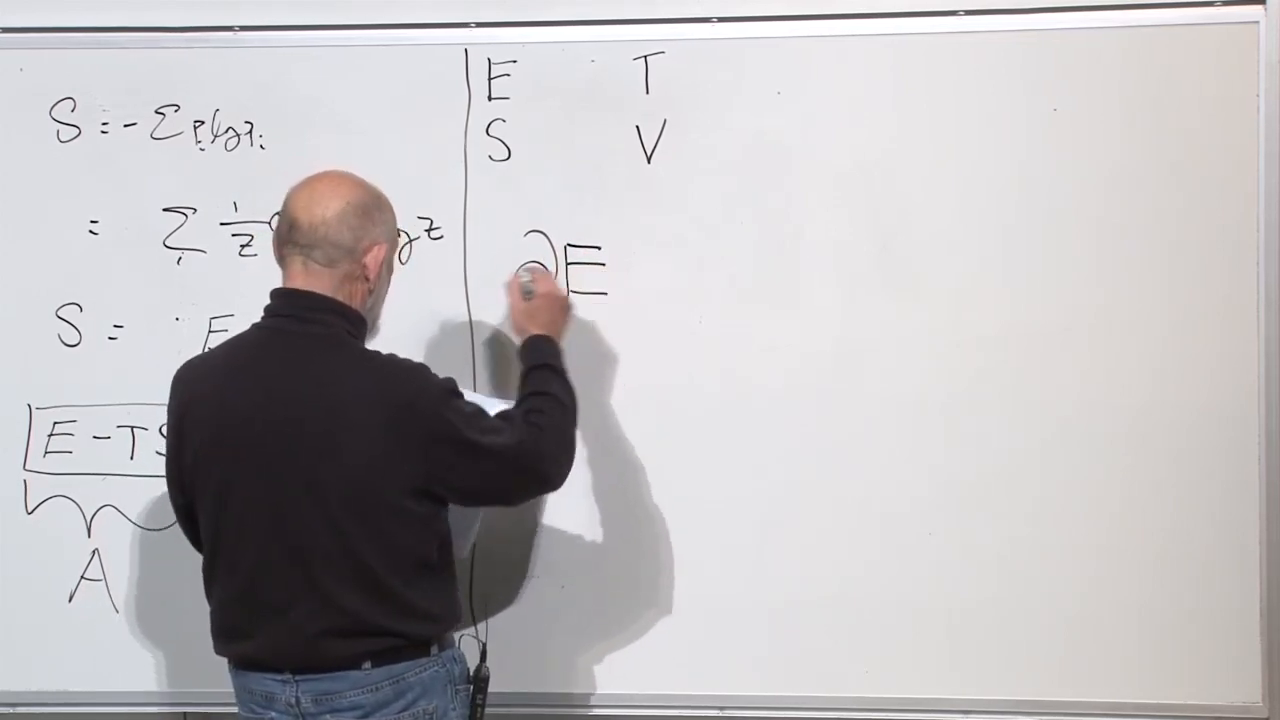
\includegraphics[width=0.90\textwidth]{lecture_05_figure_03.png}
\caption{將正則系綜的熵關係整理成
\(A=E-TS=-T\log Z\)。}
\lectureframe{00:16:50}
\end{figure}

\section{控制參數及其響應}

控制參數是實驗者能從外部改變的巨觀量。移動活塞可以改變體積，而不必操控個別分子。外加電場和磁場也是例子。在更一般的系綜中，粒子數也可以允許改變。

熱力學變數自然會成對出現，彼此互為共軛變數。在這個問題中，體積是控制參數，壓力則是它的響應。我們改變\(V\)；壓力則反映系統在能量上如何抵抗這項改變。稍後，能量的導數會明確說明這種配對關係。

\begin{classroomqa}
\audiencequestion{壓力本身可以視為控制參數嗎？}
\lecturerresponse{可以設計一種固定外部壓力的實驗；但在這裡採用的設定中，活塞位置決定體積，內部壓力則是響應量。壓力和體積互為共軛變數；控制哪一個，取決於所採用的系綜與裝置。
\lecturetimestamp{00:19:22--00:20:01}}
\end{classroomqa}

\begin{classroomqa}
\audiencequestion{這裡假設所有分子都相同嗎？還是這套論證只適用於氣體？}
\lecturerresponse{熱力學論證不需要這些限制。圓筒中可以有多種粒子、液體，甚至正在受壓的固體。一般壓力公式建立之後，理想氣體的配分函數才會作為一個特例出現。
\lecturetimestamp{00:20:02--00:20:39}}
\end{classroomqa}

\begin{classroomqa}
\audiencequestion{物質的量也可以透過另一種外部操作來改變嗎？}
\lecturerresponse{可以。粒子數也是一種可能的控制參數。若讓它動態改變，就會有相應的共軛變數，也就是化學勢。今晚的計算中，\(N\)維持不變。
\lecturetimestamp{00:20:39--00:20:57}}
\end{classroomqa}

\begin{classroomqa}
\audiencequestion{液態水和水蒸氣能同時處於平衡嗎？}
\lecturerresponse{可以，只要處於共存的溫度與壓力下。重力可能使液體位於蒸氣下方，但兩相仍可以具有相同溫度，並維持熱平衡。同一套一般性的統計力學架構也適用於此。
\lecturetimestamp{00:20:59--00:21:36}}
\end{classroomqa}

接下來的推導中，將能量和熵視為兩個獨立可調變數的函數：
\begin{equation}
 E=E(T,V),
 \qquad
 S=S(T,V).
 \label{eq:sm5-dependent-functions}
\end{equation}
溫度和體積是熱力學狀態空間的座標。能量和熵則為該空間中的每個平衡點指定數值。

\section{定熵導數}

我們最後需要的導數並不尋常：
\[
 \left(\frac{\partial E}{\partial V}\right)_S.
\]
雖然\(T\)和\(V\)是獨立座標，這個導數卻要求我們在改變\(V\)時，約束依賴函數\(S(T,V)\)維持不變。它是沿著\((T,V)\)平面中某條曲線的導數，而不是沿座標軸的導數。

\begin{classroomqa}
\audiencequestion{既然後面會用到導數\(dT/dV\)，\(T\)和\(V\)怎麼還能是獨立的？}
\lecturerresponse{在完整的狀態空間中，兩者是獨立的。施加約束\(S(T,V)=\mathrm{constant}\)後，允許的狀態便落在一維等值曲線上。沿著這條曲線，\(T\)成為\(V\)的函數，因此其斜率\(dT/dV\)有明確定義。
\lecturetimestamp{01:01:18--01:02:09}}
\end{classroomqa}

\begin{lemma}
如果\(E(T,V)\)和\(S(T,V)\)可微，則在\((\partial S/\partial T)_V\neq0\)成立的地方，
\begin{equation}
 \left(\frac{\partial E}{\partial V}\right)_S
 =
 \left(\frac{\partial E}{\partial V}\right)_T
 -
 \left(\frac{\partial E}{\partial S}\right)_V
 \left(\frac{\partial S}{\partial V}\right)_T.
 \label{eq:sm5-calculus-lemma}
\end{equation}
\end{lemma}

\begin{proof}
對於任意無窮小位移，
\begin{equation}
 dE=
 \left(\frac{\partial E}{\partial V}\right)_T dV
 +
 \left(\frac{\partial E}{\partial T}\right)_V dT.
 \label{eq:sm5-total-differential-e}
\end{equation}
在固定\(V\)時，可以依照鏈鎖律以\(S\)作為中間變數：
\begin{equation}
 \left(\frac{\partial E}{\partial T}\right)_V
 =
 \left(\frac{\partial E}{\partial S}\right)_V
 \left(\frac{\partial S}{\partial T}\right)_V.
 \label{eq:sm5-chain-rule-e-s-t}
\end{equation}

現在將位移限制在\(S\)維持不變的等值曲線上。沿著這條曲線，
\begin{equation}
 0=dS=
 \left(\frac{\partial S}{\partial V}\right)_T dV
 +
 \left(\frac{\partial S}{\partial T}\right)_V dT.
 \label{eq:sm5-constant-entropy-differential}
\end{equation}
解出曲線的斜率，可得
\begin{equation}
 \left(\frac{dT}{dV}\right)_S
 =
 -
 \frac{\left(\frac{\partial S}{\partial V}\right)_T}
 {\left(\frac{\partial S}{\partial T}\right)_V}.
 \label{eq:sm5-entropy-contour-slope}
\end{equation}
將\eqref{eq:sm5-total-differential-e}除以\(dV\)，利用
\eqref{eq:sm5-chain-rule-e-s-t}，再代入
\eqref{eq:sm5-entropy-contour-slope}：
\begin{align}
 \left(\frac{\partial E}{\partial V}\right)_S
 &=
 \left(\frac{\partial E}{\partial V}\right)_T
 +
 \left(\frac{\partial E}{\partial S}\right)_V
 \left(\frac{\partial S}{\partial T}\right)_V
 \left(\frac{dT}{dV}\right)_S \notag\\
 &=
 \left(\frac{\partial E}{\partial V}\right)_T
 -
 \left(\frac{\partial E}{\partial S}\right)_V
 \left(\frac{\partial S}{\partial V}\right)_T.
\end{align}
因子\((\partial S/\partial T)_V\)已經消去，證明得證。
\end{proof}

\begin{figure}[t]
\centering
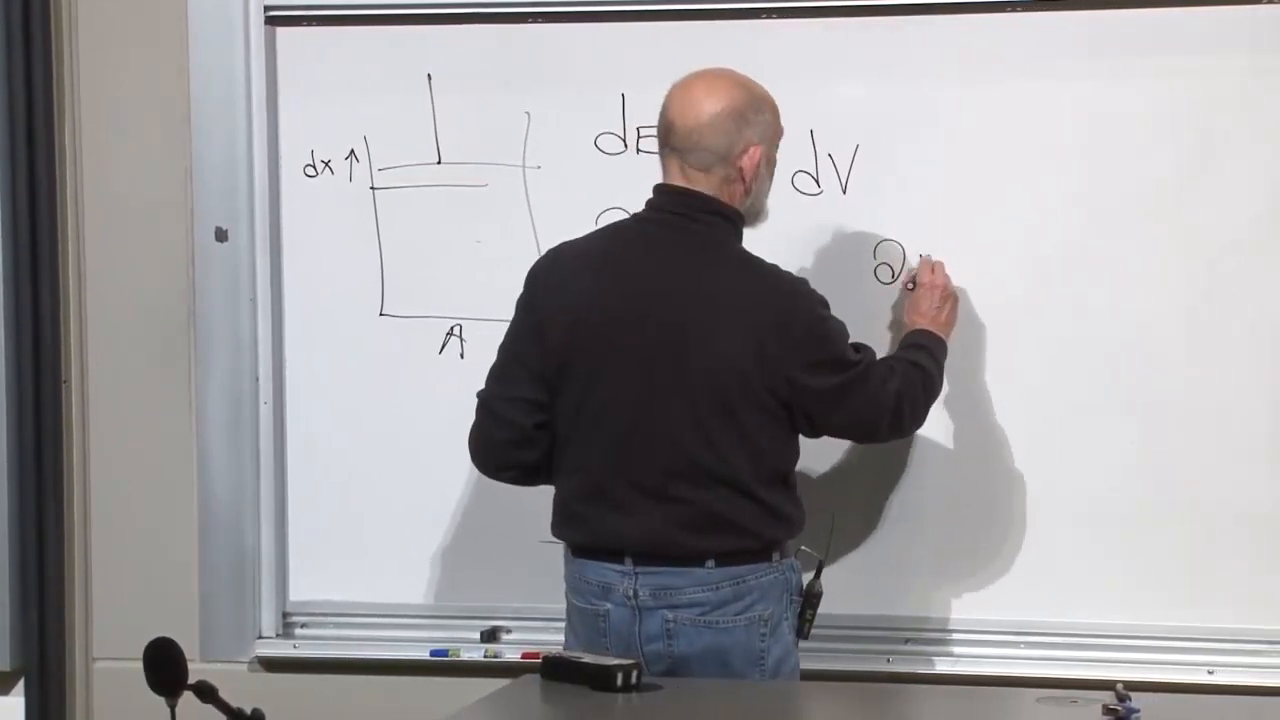
\includegraphics[width=0.90\textwidth]{lecture_05_figure_04.png}
\caption{定熵等值曲線上的計算，以及完成導數引理的消去步驟。}
\lectureframe{00:36:10}
\end{figure}

幾何圖像並非裝飾。它說明了為什麼看似奇特的固定\(S\)導數，可以用獨立座標\(T\)和\(V\)下的普通偏導數來計算。在推導中寫出\(\delta E/\delta V\)，也能提醒我們：這些符號代表沿指定路徑的小變化之比。

\begin{classroomqa}
\audiencequestion{\(dE\)的展開只是偏導數的一般定義嗎？}
\lecturerresponse{是的。全微分並沒有什麼特殊之處。唯一額外的步驟，是接著限制在等值曲線\(dS=0\)上；這會決定\(dT\)和\(dV\)之間的關係。
\lecturetimestamp{00:29:26--00:29:32}}
\end{classroomqa}

\begin{classroomqa}
\audiencequestion{消去時是否要求\((\partial S/\partial T)_V\)不為零？}
\lecturerresponse{是的。對一般的穩定系統，
\[
 \left(\frac{\partial S}{\partial T}\right)_V
 =\frac{C_V}{T}>0,
\]
因此可以合法地進行除法。特殊點則需要另外處理。哈密頓量固定時，提高溫度會使正則系綜的能量分布變寬，熵通常也會增加；降低溫度則會使分布變窄。這才是單調性論證在物理上正確的方向。
\lecturetimestamp{00:36:50--00:37:47}}
\end{classroomqa}

\section{活塞做功與絕熱條件}

現在為這個導數賦予物理意義。考慮一個截面積為\(\mathcal A\)的活塞。若活塞向外移動\(dx\)，則
\begin{equation}
 dV=\mathcal A\,dx.
 \label{eq:sm5-piston-volume}
\end{equation}
氣體對活塞施加\(P\mathcal A\)的力，因此氣體所做的功為
\begin{equation}
 \delta W_{\mathrm{by}}=P\mathcal A\,dx=P\,dV.
 \label{eq:sm5-piston-work}
\end{equation}
若沒有熱量進入氣體，能量守恆給出
\begin{equation}
 dE=-P\,dV.
 \label{eq:sm5-adiabatic-work}
\end{equation}
這個符號反映了實際的物理過程：膨脹時，氣體推升或加速活塞，而氣體本身的能量減少。

\begin{figure}[t]
\centering
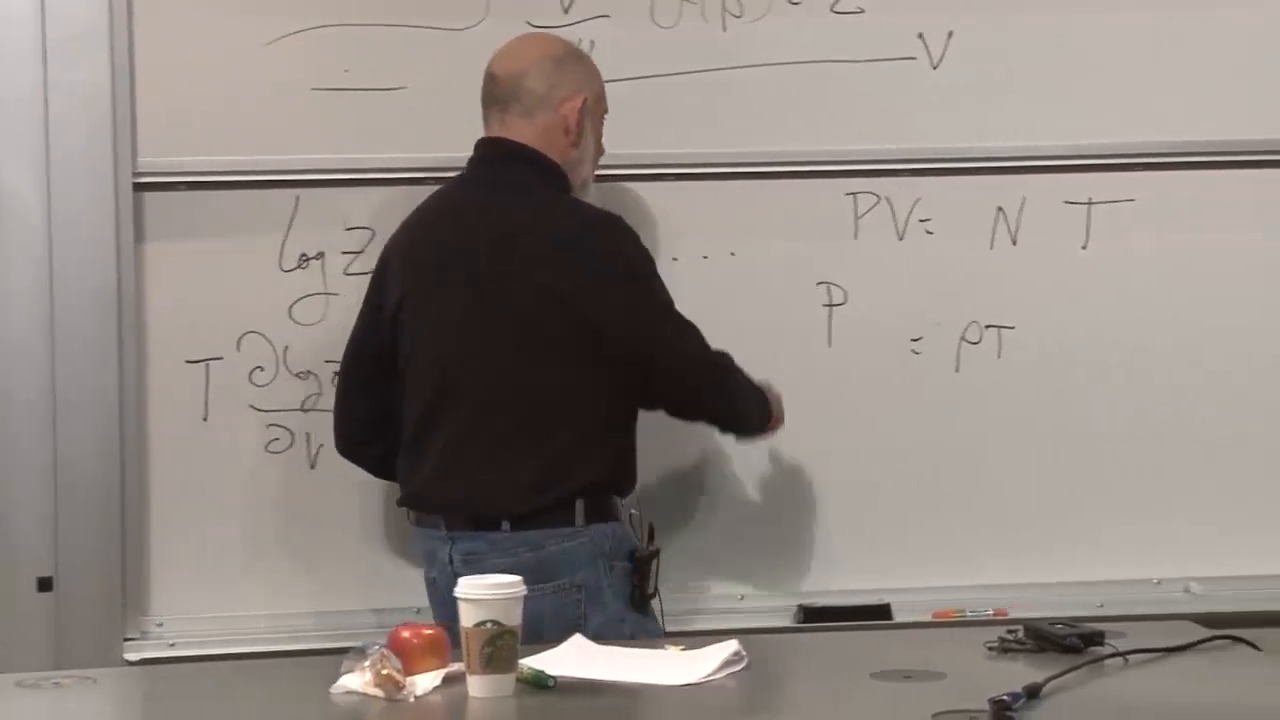
\includegraphics[width=0.90\textwidth]{lecture_05_figure_05.png}
\caption{活塞的幾何關係，以及推得的功的關係式\(dE=-P\,dV\)。}
\lectureframe{00:43:10}
\end{figure}

有兩項條件不可或缺。活塞必須移動得夠慢，讓系統始終任意接近平衡態；器壁也必須隔熱，避免能量以熱的形式進入。若拉動得很快，活塞可能在移動期間都沒有被任何分子撞到。快速壓縮則會產生衝擊波。這兩種過程都不能表示為一連串平衡態。

\emph{絕熱}一詞有時指沒有熱傳遞，有時指緩慢變化。在這裡所需的可逆過程中，兩項條件都要具備：變化是準靜態的，而且系統與外界隔熱。在這些條件下，過程也是等熵的。

\begin{classroomqa}
\audiencequestion{為什麼絕熱變化會使熵維持不變？}
\lecturerresponse{從量子力學的角度來看系統。系統的多體能階會隨體積改變。當\(V\)緩慢變化時，絕熱定理會使每個受佔據的能階連續地演變為相應的能階，而不在能階標籤之間發生躍遷。能量\(E_i(V)\)會改變，但佔據機率\(p_i\)維持不變。由於熵\(S=-\sum_i p_i\log p_i\)取決於這些機率，因此熵也維持不變。熱交換或不可逆運動則會使這個結論不再成立。
\lecturetimestamp{00:43:37--00:49:15}}
\end{classroomqa}

\begin{figure}[t]
\centering
\includegraphics[width=0.90\textwidth]{lecture_05_figure_06.png}
\caption{多體能階隨體積改變，而佔據機率仍對應於原來的能階標籤。}
\lectureframe{00:48:50}
\end{figure}

沿這條定熵路徑計算方程\eqref{eq:sm5-adiabatic-work}，即可辨認出壓力為
\begin{equation}
 P=-\left(\frac{\partial E}{\partial V}\right)_S.
 \label{eq:sm5-pressure-fixed-entropy}
\end{equation}
這就是壓力與體積之間的共軛關係。

\begin{classroomqa}
\audiencequestion{如果快速移動活塞，會發生什麼事？}
\lecturerresponse{系統會離開平衡態，此時具體的動力學過程便很重要。突然壓縮會產生衝擊波。在理想的自由膨脹中，活塞可以在分子撞上它之前就退開，因此不會做功；即使體積改變，能量仍保持不變。之後氣體會弛豫至熵增加的平衡態。這類過程無法用\eqref{eq:sm5-pressure-fixed-entropy}中的單一平衡態導數來描述。
\lecturetimestamp{00:58:30--01:01:15}}
\end{classroomqa}

\begin{classroomqa}
\audiencequestion{要用什麼定量條件判斷變化是否緩慢？}
\lecturerresponse{外部變化的時間尺度必須遠大於相關的內部弛豫時間。對氣體而言，在巨觀變化期間應該發生許多次分子碰撞和器壁碰撞。確切的時間尺度取決於物質和幾何形狀；準靜態極限本身則具有普遍性。
\lecturetimestamp{01:02:09--01:03:20}}
\end{classroomqa}

\section{從絕熱能量到配分函數}

物理關係式\eqref{eq:sm5-pressure-fixed-entropy}還不是容易計算的形式。正則系綜統計力學自然以溫度為變數，因為\(T\)直接出現在波茲曼因子中。微積分引理可以將不易處理的定熵導數，轉換成適合計算的形式：
\begin{align}
 P
 &=
 -\left(\frac{\partial E}{\partial V}\right)_T
 +
 \left(\frac{\partial E}{\partial S}\right)_V
 \left(\frac{\partial S}{\partial V}\right)_T.
 \label{eq:sm5-pressure-lemma-substitution}
\end{align}
定體積下，第一定律給出\(dE=T\,dS\)，因此
\begin{equation}
 \left(\frac{\partial E}{\partial S}\right)_V=T.
 \label{eq:sm5-e-s-temperature}
\end{equation}
於是
\begin{equation}
 P=
 -\left(\frac{\partial E}{\partial V}\right)_T
 +
 T\left(\frac{\partial S}{\partial V}\right)_T.
 \label{eq:sm5-pressure-fixed-temperature-pieces}
\end{equation}

\begin{classroomqa}
\audiencequestion{壓力公式中的負號從何而來？}
\lecturerresponse{負號源自氣體所做的功：在絕熱膨脹過程中，\(dE=-P\,dV\)。微積分引理的兩項之間本身就有一個負號；而\(P=-(\partial E/\partial V)_S\)中的整體負號會使兩項的符號都反轉，得到
\eqref{eq:sm5-pressure-fixed-temperature-pieces}。
\lecturetimestamp{00:52:40--00:53:14}}
\end{classroomqa}

兩個導數都在固定\(T\)的條件下計算，因此
\begin{align}
 P
 &=
 -\left(\frac{\partial}{\partial V}(E-TS)\right)_T \notag\\
 &=
 -\left(\frac{\partial A}{\partial V}\right)_T.
 \label{eq:sm5-pressure-free-energy}
\end{align}
最後代入\(A=-T\log Z\)：
\begin{equation}
 \boxed{
 P=
 T\left(\frac{\partial\log Z}{\partial V}\right)_T
 }.
 \label{eq:sm5-pressure-log-z}
\end{equation}

\begin{figure}[t]
\centering
\includegraphics[width=0.90\textwidth]{lecture_05_figure_07.png}
\caption{將推導整理為定溫下的形式：
\(P=-(\partial A/\partial V)_T
=T(\partial\log Z/\partial V)_T\)。}
\lectureframe{00:55:55}
\end{figure}

\eqref{eq:sm5-pressure-log-z}並未假設氣體是理想氣體。只要能算出交互作用流體、電漿或固體的配分函數，同一個導數就能給出其壓力。更一般地，每個外部控制參數都有一個共軛響應量，可藉由對適當的熱力學勢求導得到。配分函數包含了許多這類響應量：對\(\log Z\)關於\(\beta\)求導會得到能量，對體積求導則會得到壓力。

\section{理想氣體狀態方程式}

現在才限定為\(N\)個互不作用的粒子。保留經典相空間的歸一化因子，
\begin{equation}
 Z_N=
 \frac{1}{N!h^{3N}}
 \int d^{3N}q\,d^{3N}p\,
 \exp\!\left[
 -\beta\sum_{a=1}^{N}\frac{\mathbf p_a^2}{2m}
 \right].
 \label{eq:sm5-ideal-gas-partition-integral}
\end{equation}
其中有\(3N\)個位置座標和\(3N\)個動量座標。哈密頓量與位置無關，因此每個粒子都會貢獻一個容器體積因子：
\begin{equation}
 Z_N=
 \frac{V^N}{N!h^{3N}}I_p(\beta),
 \label{eq:sm5-ideal-gas-factorization}
\end{equation}
其中整個動量積分\(I_p(\beta)\)與\(V\)無關。

\begin{classroomqa}
\audiencequestion{為什麼位置積分和動量積分各有\(3N\)\(3N\)個？}
\lecturerresponse{每個\(N\)粒子都有三個空間座標和三個共軛動量分量。相空間的每一半各有\(3N\)個座標，而不是\(N\)個粒子再加上另外\(3N\)個粒子。
\lecturetimestamp{01:04:19--01:04:28}}
\end{classroomqa}

取對數後，體積的依賴關係就分離出來：
\begin{equation}
 \log Z_N
 =
 N\log V-\log N!-3N\log h+\log I_p(\beta).
 \label{eq:sm5-log-ideal-gas-partition}
\end{equation}
因子\(1/N!\)、\(h^{-3N}\)和\(I_p(\beta)\)都與體積無關。它們會影響絕對熵等其他問題，但不影響這裡要計算的導數。因此
\begin{equation}
 \left(\frac{\partial\log Z_N}{\partial V}\right)_T
 =\frac{N}{V}.
 \label{eq:sm5-log-z-volume-derivative}
\end{equation}
由方程\eqref{eq:sm5-pressure-log-z}可立即得到
\begin{equation}
 P=\frac{NT}{V},
 \qquad
 \boxed{PV=NT}.
 \label{eq:sm5-ideal-gas-law}
\end{equation}

\begin{classroomqa}
\audiencequestion{\(N\)還包含推導波茲曼分布時使用的複本嗎？}
\lecturerresponse{不包含。複本構造只是先前推導中用來計數的工具，這裡已不再使用。此處的\(N\)是這一份氣體樣本中的實際粒子數。
\lecturetimestamp{01:07:38--01:08:05}}
\end{classroomqa}

定義數密度
\begin{equation}
 \rho=\frac{N}{V}
 \label{eq:sm5-number-density}
\end{equation}
便可得到等價的形式
\begin{equation}
 P=\rho T.
 \label{eq:sm5-density-equation-of-state}
\end{equation}

\begin{classroomqa}
\audiencequestion{要得到密度形式，應該除以\(N\)還是\(V\)？}
\lecturerresponse{將\(PV=NT\)除以\(V\)：
\(P=(N/V)T=\rho T\)。這裡的\(\rho\)是數密度，不是質量密度。
\lecturetimestamp{01:08:45--01:09:16}}
\end{classroomqa}

\begin{figure}[t]
\centering
\includegraphics[width=0.90\textwidth]{lecture_05_figure_08.png}
\caption{\(\log Z\)對體積的導數，以及由此得到的理想氣體狀態方程式\(PV=NT\)，也就是\(P=\rho T\)。}
\lectureframe{01:09:25}
\end{figure}

改回實驗室使用的溫度\(T_K\)，
\begin{equation}
 PV=Nk_BT_K.
 \label{eq:sm5-ideal-gas-law-laboratory}
\end{equation}
這個熟悉的結果與動力學直覺一致，但如今它的推導所依據的架構，適用範圍遠超過自由氣體。

\section{另一個收穫：平衡漲落}

壓力的推導已經完成，但還有一個先前提出的問題尚未回答：配分函數還能提供什麼資訊？考慮一個與熱浴接觸的系統。它的能量並非固定不變，而是會進出系統；因此重複測量時，能量會在正則系綜的平均值附近漲落。

\begin{classroomqa}
\audiencequestion{現在可以計算先前提到的漲落了嗎？}
\lecturerresponse{可以。還有時間再說明一次相同的原理：\(Z\)的導數蘊含可測量的熱力學資訊。
\lecturetimestamp{01:10:37--01:10:50}}
\end{classroomqa}

\subsection{變異數與標準差}

對於隨機變數\(x\)，若\(\langle x\rangle=0\)，則可用\(\langle x^2\rangle\)衡量分布的寬度。對於一般分布，先將變數減去其平均值：
\begin{equation}
 \delta x=x-\langle x\rangle.
 \label{eq:sm5-centered-variable}
\end{equation}
所得變數的平均值為零：
\begin{equation}
 \langle\delta x\rangle
 =
 \langle x\rangle-\langle x\rangle=0,
 \label{eq:sm5-centered-mean}
\end{equation}
其均方為
\begin{align}
 (\Delta x)^2
 &\equiv
 \left\langle\left(x-\langle x\rangle\right)^2\right\rangle \notag\\
 &=
 \langle x^2\rangle
 -2\langle x\rangle^2
 +\langle x\rangle^2 \notag\\
 &=
 \langle x^2\rangle-\langle x\rangle^2.
 \label{eq:sm5-variance}
\end{align}
這就是變異數。變異數的正平方根\(\Delta x\)則是標準差。

\begin{classroomqa}
\audiencequestion{為什麼\(x-\langle x\rangle\)的平均值恰好等於零？}
\lecturerresponse{平均值具有線性，而\(\langle x\rangle\)本身已是數值。因此
\(\langle x-\langle x\rangle\rangle
=\langle x\rangle-\langle x\rangle=0\)。
\lecturetimestamp{01:14:02--01:14:22}}
\end{classroomqa}

\begin{classroomqa}
\audiencequestion{平方漲落、變異數、均方根寬度和標準差有什麼區別？}
\lecturerresponse{變異數是
\((\Delta x)^2=\langle x^2\rangle-\langle x\rangle^2\)。
標準差是變異數的平方根，即\(\Delta x\)。對於平均值為零的變數，標準差也等於其均方根值。
\lecturetimestamp{01:16:39--01:18:38}}
\end{classroomqa}

\begin{figure}[t]
\centering
\includegraphics[width=0.90\textwidth]{lecture_05_figure_09.png}
\caption{平移後的變數，以及推得\((\Delta x)^2=\langle x^2\rangle-\langle x\rangle^2\)的展開式。}
\lectureframe{01:17:20}
\end{figure}

\subsection{由配分函數求得能量矩}

對於正則系綜，
\begin{align}
 \langle E\rangle
 &=
 \frac{1}{Z}\sum_i E_i e^{-\beta E_i} \notag\\
 &=
 -\frac{1}{Z}\frac{\partial Z}{\partial\beta}
 =
 -\frac{\partial\log Z}{\partial\beta}.
 \label{eq:sm5-mean-energy-from-z}
\end{align}
乘上一個\(E_i\)因子，相當於對\(\beta\)求一次負導數。再求一次導數，就會得到\(E_i^2\)：
\begin{equation}
 \langle E^2\rangle
 =
 \frac{1}{Z}\sum_i E_i^2e^{-\beta E_i}
 =
 \frac{1}{Z}\frac{\partial^2 Z}{\partial\beta^2}.
 \label{eq:sm5-second-energy-moment}
\end{equation}
因此，能量的變異數為
\begin{align}
 (\Delta E)^2
 &=
 \langle E^2\rangle-\langle E\rangle^2 \notag\\
 &=
 \frac{1}{Z}\frac{\partial^2Z}{\partial\beta^2}
 -
 \frac{1}{Z^2}
 \left(\frac{\partial Z}{\partial\beta}\right)^2 \notag\\
 &=
 \frac{\partial^2\log Z}{\partial\beta^2}
 =
 -\frac{\partial\langle E\rangle}{\partial\beta}.
 \label{eq:sm5-energy-variance-beta}
\end{align}
再次可見，看似複雜的可觀測量其實可以寫成\(\log Z\)的導數。

\begin{figure}[t]
\centering
\includegraphics[width=0.90\textwidth]{lecture_05_figure_10.png}
\caption{將\(\beta\)的二階導數\(\log Z\)與能量變異數連結起來。}
\lectureframe{01:29:00}
\end{figure}

\subsection{熱容量與漲落的大小}

以本講採用的單位表示，\(T=1/\beta\)，因此
\begin{equation}
 -\frac{\partial}{\partial\beta}
 =
 T^2\frac{\partial}{\partial T}.
 \label{eq:sm5-beta-temperature-derivative}
\end{equation}
定義整個樣本在定體積下的熱容量為
\begin{equation}
 C_V\equiv
 \left(\frac{\partial\langle E\rangle}{\partial T}\right)_V.
 \label{eq:sm5-heat-capacity}
\end{equation}
方程\eqref{eq:sm5-energy-variance-beta}便成為
\begin{equation}
 \boxed{(\Delta E)^2=T^2C_V}
 \qquad (k_B=1).
 \label{eq:sm5-energy-fluctuation-lecture-units}
\end{equation}
若改用實驗室溫度\(T_K\)，其中
\(\beta=(k_BT_K)^{-1}\)，則有
\begin{equation}
 \boxed{(\Delta E)^2=k_BT_K^2C_V}.
 \label{eq:sm5-energy-fluctuation-laboratory}
\end{equation}

\begin{figure}[t]
\centering
\includegraphics[width=0.90\textwidth]{lecture_05_figure_11.png}
\caption{從\(\beta\)導數轉換為定容熱容量，並恢復\(k_B\)因子。}
\lectureframe{01:31:10}
\end{figure}

\begin{classroomqa}
\audiencequestion{導數必須指定在定體積下，而不是定壓下嗎？}
\lecturerresponse{是的。這個正則系綜的推導會固定哈密頓量的外部控制參數，包括\(V\)。因此得到的量是\(C_V\)。定壓系綜允許體積和功發生漲落，並且需要使用相應的熱力學勢；不能只在\eqref{eq:sm5-energy-fluctuation-laboratory}中把\(C_V\)換成\(C_P\)。
\lecturetimestamp{01:29:01--01:29:28; 01:32:50--01:33:21}}
\end{classroomqa}

\begin{classroomqa}
\audiencequestion{\(C_V\)是材料常數嗎？}
\lecturerresponse{一般而言不是。它可能隨溫度、體積、相態和組成而變。此外，這裡的\(C_V\)是整個樣本的熱容量，屬於廣延量。只有再除以質量、粒子數或物質的量，才會得到比熱或莫耳熱容量。
\lecturetimestamp{01:31:47--01:32:21; 01:33:23--01:34:55}}
\end{classroomqa}

對一般的廣延物質，\(C_V\)與\(N\)成正比，因此\((\Delta E)^2\)與\(N\)成正比，而\(\Delta E\)與\(\sqrt{N}\)成正比。平均能量本身則與\(N\)成正比。因此
\begin{equation}
 \frac{\Delta E}{\langle E\rangle}\sim\frac{1}{\sqrt{N}}.
 \label{eq:sm5-relative-fluctuation-scaling}
\end{equation}
巨觀系統的相對漲落非常小，微觀樣本則能直接呈現這些漲落。\(k_B\)出現在\eqref{eq:sm5-energy-fluctuation-laboratory}中，顯示熱力學可觀測量與分子的離散性相連；換句話說，它也連結了巨觀單位與阿伏加德羅數量級的計數。

壓力與漲落如今都從同一個量導出：
\[
 P=T\left(\frac{\partial\log Z}{\partial V}\right)_T,
 \qquad
 (\Delta E)^2=\frac{\partial^2\log Z}{\partial\beta^2}.
\]
這是本講的核心要點。辨明正確的約束條件後，配分函數便不只是用來將機率歸一化；它的導數也系統地整理出可測量的熱力學性質。
\chapter{弱相互作用、維里修正與非恰當微分}

\lectureoverview{我們先從測量與溫度的操作性意義談起，再探討短程相互作用微弱地開啟時，稀薄氣體如何偏離理想氣體定律。配分函數給出能量與壓力的首階相互作用修正，並指出其適用範圍。最後的數學插曲以恰當微分、閉合迴路和一個具體的理想氣體例子，區分態函數與依賴路徑的熱和功。}

\section{儀器實際測量的是什麼}

沒有任何實驗室儀器能直接探入自然，讀出抽象的數學變數。彈簧秤讀出伸長量；溫度計讀出液柱高度。我們之所以稱前者為力的測量、後者為溫度的測量，只是因為可觀察到的響應與所要測量的量之間，已建立可重複的關係。

這種關係有其適用範圍。彈簧只有在保持彈性時才遵循虎克定律；施加的力夠大時，最終會使彈簧變形或斷裂。更一般地，若平滑的讀值\(R\)取決於物理變數\(X\)，則在選定的操作點附近，
\begin{equation}
 \Delta R \simeq
 \left.\frac{dR}{dX}\right|_{X_0}\Delta X.
 \label{eq:sm6-local-linear-response}
\end{equation}
即使完整的響應曲線是非線性的，讀值的小變化仍與目標變數的小變化成正比。這種局部線性化正是一般校準的原理。

讀值也可能受到干擾變數影響。彈簧可能會微弱地響應溫度或壓力。溫度計中水銀柱的高度可能因重力而隨方向改變，也可能受玻璃性質或材料緩慢變化的影響。測量程序並不能證明這些依賴關係不存在；它會將相關因素固定，或確認這些因素在所需的尺度上可以忽略。

\begin{classroomqa}
\audiencequestion{局部重力場，或溫度計拿持的方向，會改變讀值嗎？}
\lecturerresponse{原則上會。如果方向造成的影響不可忽略，將溫度計保持垂直的指示就成為儀器定義的一部分。在地球表面附近，重力場相當穩定，因此剩餘的變化通常可以忽略。
\lecturetimestamp{00:04:08--00:05:00}}
\end{classroomqa}

\begin{classroomqa}
\audiencequestion{老化或化學變化會不會逐漸改變校準？}
\lecturerresponse{有可能。對一般測量而言，水銀和玻璃都足夠惰性；而時間尺度極長的變化，與實驗無關。校準始終是針對特定儀器、範圍、程序和時長所作的說明。
\lecturetimestamp{00:05:03--00:06:11}}
\end{classroomqa}

攝氏溫度計以兩個可重複的參考狀態，建立方便的溫標。若\(h_f\)和\(h_b\)分別是水在凝固點和沸點時的液柱高度，則在響應近似線性的範圍內，
\begin{equation}
 T_{\mathrm C}=100\,\frac{h-h_f}{h_b-h_f}.
 \label{eq:sm6-celsius-calibration}
\end{equation}
將凝固點定為\(T_{\mathrm C}=0\)是約定俗成的選擇。這並不代表熱能為零，正如冬日的華氏零度並非絕對零度。

\begin{figure}[t]
\centering
\includegraphics[width=0.90\textwidth]{lecture_06_figure_03.png}
\caption{平滑但非線性的溫度計響應；其中一小段區間標示為線性校準範圍。}
\lectureframe{00:07:55}
\end{figure}

\section{平衡與作為能量尺度的溫度}

只有當溫度計與周圍介質達到熱平衡後，它測得的才是周遭環境的溫度。在此之前，讀值只是在逐漸趨近平衡。實際的判準很簡單：等到讀值不再變化。這條規則看似簡單，卻掩蓋了決定等待時間的物理過程。

\begin{classroomqa}
\audiencequestion{達到平衡是否只涉及球泡周圍的邊界層？又該等多久？}
\lecturerresponse{能量必須穿過玻璃，並與周圍介質交換，因此所需時間取決於溫度計、它的熱導率以及介質。緊鄰溫度計的環境也必須能代表均勻的平衡狀態。實驗上，讀值不再漂移時，就可接受該讀值。
\lecturetimestamp{00:08:45--00:10:13}}
\end{classroomqa}

在這段等待時間裡，溫度和密度扮演不同的角色。極稀薄的氣體也可能非常熱：其中少數分子可能具有很大的動能。然而，這些分子很少撞擊溫度計，因此達到平衡可能要花很久。在溫度不變的情況下將密度降低一百倍或一千倍，不會降低分子的能量尺度；降低的是能量傳遞到儀器的速率。

\begin{classroomqa}
\audiencequestion{房間裡的輻射溫度會與空氣溫度不同嗎？}
\lecturerresponse{會。物質和輻射只有彼此達到熱平衡時，才會具有相同的溫度。中性空氣與照明房間中的許多光學輻射耦合微弱，因此光子分布不一定是處於空氣溫度下的平衡黑體輻射場。
\lecturetimestamp{00:11:26--00:12:20}}
\end{classroomqa}

達到平衡後，最好將溫度視為能量尺度。我們仍採用\(k_B=1\)的單位制，因此\(T\)本身具有能量的量綱。對單原子理想氣體而言，
\begin{equation}
 E_0=\frac{3}{2}NT.
 \label{eq:sm6-ideal-energy}
\end{equation}
每個分子的熱能由\(T\)決定；相應的速率仍取決於分子質量。

\section{開啟弱相互作用}

\begin{classroomqa}
\audiencequestion{理想氣體近似在什麼條件下會失效？能否用數學方式呈現這種失效？}
\lecturerresponse{從已求解的非相互作用氣體出發，逐漸加入微弱相互作用。對這項變化作展開，計算首階修正，並與理想氣體項比較。當修正不再微小時，近似便會失效。
\lecturetimestamp{00:12:25--00:14:40}}
\end{classroomqa}

這是標準的微擾策略。如果一個問題在\(\lambda=0\)時可解，就引入耦合常數\(\lambda\)，寫成
\begin{equation}
 F(\lambda)=F(0)+\lambda F_1+\lambda^2F_2+\cdots,
 \label{eq:sm6-perturbative-template}
\end{equation}
再檢視保留的每一項是否都小於前一項。此處的參考問題是理想氣體。物理上的小量來自樣品稀薄、相互作用範圍比平均粒子間距短，以及勢夠弱，使首階相互作用項具有參考價值。即使單次相遇看來影響不大，高密度或長程力仍可能使近似失效。

令\(x_i\in\mathbb R^3\)和\(p_i\in\mathbb R^3\)分別表示分子\(i\)的位置和動量。對質量為\(m\)的相同分子，取
\begin{equation}
 H(X,P)=
 \sum_{i=1}^{N}\frac{p_i^2}{2m}
 +\sum_{i<j}u\!\left(|x_i-x_j|\right),
 \label{eq:sm6-interacting-hamiltonian}
\end{equation}
其中\(X=(x_1,\ldots,x_N)\)，\(P=(p_1,\ldots,p_N)\)。限制\(i<j\)排除粒子與自身配對，並使每個\((i,j)\)只計算一次：
\begin{equation}
 \sum_{i<j}1=\binom{N}{2}=\frac{N(N-1)}{2}.
 \label{eq:sm6-pair-count}
\end{equation}

\begin{classroomqa}
\audiencequestion{為什麼不分別對兩個粒子標籤求和？}
\lecturerresponse{\((3,7)\)和\((7,3)\)代表同一個物理粒子對，而且粒子不會與自身配對。將求和限制為\(i<j\)，便同時確保這兩點。質量仍以\(m\)表示，而\(i,j\)用來標記粒子，避免\(m\)同時用於兩種用途時產生符號混淆。
\lecturetimestamp{00:17:52--00:19:12}}
\end{classroomqa}

總組態勢能寫成
\begin{equation}
 U(X)=\sum_{i<j}u\!\left(|x_i-x_j|\right).
 \label{eq:sm6-total-potential}
\end{equation}
假設相互作用具有平移不變性且為短程：當距離\(r\)遠大於分子尺度時，\(u(r)\)可忽略。

\section{積分後的粒子對作用強度}

弱粒子對勢只有一個積分會進入首階修正：
\begin{equation}
 U_0\equiv\int_{\mathbb R^3}d^3r\,u(r).
 \label{eq:sm6-u0-definition}
\end{equation}
其單位是能量乘以體積。這個積分結合了相互作用的典型強度，以及相互作用顯著的空間範圍。

\begin{figure}[t]
\centering
\includegraphics[width=0.90\textwidth]{lecture_06_figure_04.png}
\caption{以積分強度\(U_0=\int d^3r\,u(r)\)概括短程粒子對勢。}
\lectureframe{00:25:15}
\end{figure}

看看\(U_0\)為何有用，可以先考慮一個粒子對：
\begin{equation}
 I_2=\int_V d^3x_1\,d^3x_2\,
 u\!\left(|x_1-x_2|\right).
 \label{eq:sm6-two-particle-integral}
\end{equation}
引入相對座標\(r=x_2-x_1\)。遠離邊界時，相對座標的積分給出\(U_0\)，而粒子對的共同位置可遍及整個容器。因此
\begin{equation}
 I_2=V U_0+\text{surface corrections}.
 \label{eq:sm6-pair-integral-vu0}
\end{equation}
修正來自距離壁面在一個相互作用範圍內的粒子；此時相對座標的鄰域有一部分落在盒子之外。修正的相對大小隨表面積與體積之比而變，並在宏觀極限下趨近於零。

\begin{classroomqa}
\audiencequestion{\(U_0\)是指選定的一個粒子對嗎？是否讓其中一個粒子與另一個粒子保持固定距離？}
\lecturerresponse{它指的是任一粒子對都遵循的同一相互作用定律。固定第一個粒子，對第二個粒子的所有相對位置積分；積分時兩者的距離並不固定。只有附近的相互作用區域會有顯著貢獻，因此得到\(U_0\)。
\lecturetimestamp{00:26:03--00:27:33}}
\end{classroomqa}

\begin{classroomqa}
\audiencequestion{為什麼第二個位置積分給出整個容器體積，第一個卻沒有？}
\lecturerresponse{將相對構型積分成\(U_0\)後，整個粒子對就能在樣品中平移。這種共同平移帶來大的因子\(V\)。相互作用鄰域的體積只有分子尺度，而且已包含在\(U_0\)中；它不是另一個等於容器體積的因子。
\lecturetimestamp{00:27:48--00:29:21}}
\end{classroomqa}

\begin{classroomqa}
\audiencequestion{這個值會不會取決於固定哪個位置，尤其是在壁面附近？}
\lecturerresponse{平移不變性使體相中的值不受固定位置影響。壁面附近的積分則略有不同，因為某些鄰近位置無法取得。受到影響的只有厚度約一個分子尺度的表層，因此對宏觀尺度的盒子而言，誤差可以忽略。
\lecturetimestamp{00:29:24--00:31:22}}
\end{classroomqa}

\begin{classroomqa}
\audiencequestion{這個結果是對所有雙粒子構型積分後的勢能嗎？為什麼它只正比於一個大的體積？}
\lecturerresponse{是的。它的單位是能量乘以體積平方，因為\(V U_0\)包含一個容器體積和一個分子尺度的相互作用體積。只有前者會隨樣品大小增加。
\lecturetimestamp{00:31:31--00:32:04}}
\end{classroomqa}

\begin{classroomqa}
\audiencequestion{在固定體積下，球形容器的表面積最小；選球形會改變體相答案嗎？}
\lecturerresponse{只會改變微小的邊界修正。對任何一般的宏觀形狀，距離表面不到一個分子尺度的粒子數，相較於體相中的粒子數可以忽略。只有當容器本身接近分子尺度時，表面效應才會變得重要。
\lecturetimestamp{00:32:04--00:33:58}}
\end{classroomqa}

\begin{classroomqa}
\audiencequestion{用勢能取代粒子軌跡，是否就忽略了碰撞？}
\lecturerresponse{沒有。力是勢能的導數，正是這個力造成碰撞。平衡態統計力學不要求我們逐一追蹤碰撞；碰撞的影響已編碼在能量中，因此也編碼在波茲曼權重中。
\lecturetimestamp{00:33:59--00:35:29}}
\end{classroomqa}

\begin{classroomqa}
\audiencequestion{保留粒子對作用力、卻不納入真正的三體相互作用，會漏掉什麼？}
\lecturerresponse{微觀能量可能包含真正的三體項，而粒子對勢的高階項也會產生多粒子關聯。然而在稀薄氣體中，指定的三個粒子同時位於同一分子尺度鄰域的機率遠低於兩個粒子的情況。因此，粒子對效應給出首階密度修正；更高階的群集項則以更高次的密度冪次出現。
\lecturetimestamp{00:35:29--00:38:14}}
\end{classroomqa}

\section{配分函數的直接推導}

統計方法的優勢至此已很清楚。一旦哈密頓量確定，就不必猜測壁面附近或碰撞過程中的詳細速度分布。我們寫下正則配分函數，接著進行代數推導：
\begin{equation}
\begin{aligned}
 Z&=
 \frac{1}{N!h^{3N}}
 \int d^{3N}P\,d^{3N}X\\
 &\qquad{}\times e^{-\beta K(P)}e^{-\beta U(X)},\\
 K(P)&=\sum_i\frac{p_i^2}{2m}.
\end{aligned}
 \label{eq:sm6-full-partition-function}
\end{equation}
因子\(h^{3N}\)使經典相空間測度成為無因次量，而\(N!\)則消除全同粒子的置換重複計數。

\begin{figure}[t]
\centering
\includegraphics[width=0.90\textwidth]{lecture_06_figure_05.png}
\caption{多粒子能量，以及配分函數中相應的動能因子和組態因子。}
\lectureframe{00:40:35}
\end{figure}

動量和位置變數可以分離。將組態積分乘以並除以\(V^N\)，即可分離出理想氣體的結果：
\begin{align}
 Z
 &=\left[
 \frac{V^N}{N!h^{3N}}
 \int d^{3N}P\,e^{-\beta K(P)}
 \right] \notag\\
 &\quad\times\left[
 \frac{1}{V^N}
 \int d^{3N}X\,e^{-\beta U(X)}
 \right] \notag\\
 &\equiv Z_0\,C(\beta,V,N).
 \label{eq:sm6-z-factorization}
\end{align}
熟知的高斯因子為
\begin{equation}
 \int d^{3N}P\,e^{-\beta K(P)}
 =\left(\frac{2\pi m}{\beta}\right)^{3N/2}.
 \label{eq:sm6-gaussian-factor}
\end{equation}

\begin{figure}[t]
\centering
\includegraphics[width=0.90\textwidth]{lecture_06_figure_06.png}
\caption{從正規化的組態因子中分離出的理想氣體配分函數。}
\lectureframe{00:43:45}
\end{figure}

因子\(N!\)不會影響正規化比值\(C\)，也不會影響下文所用的特定固定\(N\)偏導數；但它對整體熱力學不可或缺，因為正確的狀態計數和廣延熵都需要它。

取相互作用的一階近似，
\begin{equation}
 e^{-\beta U(X)}
 =1-\beta U(X)+O(U^2).
 \label{eq:sm6-boltzmann-expansion}
\end{equation}
因此，
\begin{align}
 C
 &=
 1-\frac{\beta}{V^N}
 \sum_{i<j}
 \int d^{3N}X\,u(|x_i-x_j|)
 +O(U^2) \notag\\
 &=
 1-\frac{\beta}{V^N}
 \frac{N(N-1)}{2}
 V^{N-2}(V U_0)+O(U^2) \notag\\
 &=
 1-\beta\frac{N(N-1)}{2V}U_0+O(U^2).
 \label{eq:sm6-configurational-correction}
\end{align}
每個粒子對都有相同的\emph{積分}，但瞬時間距或勢能不必相同。其餘\(N-2\)個位置積分各自貢獻一個\(V\)因子。

\begin{figure}[t]
\centering
\includegraphics[width=0.90\textwidth]{lecture_06_figure_07.png}
\caption{粒子對計數、其餘座標的體積因子，以及首階組態修正\(1-\beta N^2U_0/(2V)\)。}
\lectureframe{00:53:40}
\end{figure}

\begin{classroomqa}
\audiencequestion{領先項\(1\)是否假設勢能在零距離時為零？}
\lecturerresponse{不是。它是指數展開中的零階項，與\(u(0)\)的值無關。勢能從下一項\(-\beta U(X)\)才開始出現。
\lecturetimestamp{00:46:19--00:46:48}}
\end{classroomqa}

\begin{classroomqa}
\audiencequestion{既然不同粒子對的距離不同，為什麼每一對都可以用同一個表示式代替？}
\lecturerresponse{這並不是把各粒子的對勢值視為相同。每一項都在相同的完整構型空間上積分，而且粒子標籤不會使某一對異於其他粒子對。因此這些積分的形式和數值都相同。
\lecturetimestamp{00:50:00--00:51:07}}
\end{classroomqa}

\begin{classroomqa}
\audiencequestion{粒子對的數目是\(N(N-1)/2\)還是\(N(N+1)/2\)？}
\lecturerresponse{是\(N(N-1)/2\)：選定一個粒子後，只有\(N-1\)個不同的夥伴；再除以二，便去除重複計算的反向排列。對宏觀的\(N\)而言，以\(N^2\)取代\(N(N-1)\)只會造成相對於\(1/N\)的修正。
\lecturetimestamp{00:48:33--00:49:56}}
\end{classroomqa}

由於\(\log(1-x)=-x-x^2/2-x^3/3-\cdots\)，取對數後的一階修正為
\begin{equation}
 \log Z
 =
 \log Z_0
 -\beta\frac{N(N-1)}{2V}U_0
 +O(U^2).
 \label{eq:sm6-logz-correction}
\end{equation}
當\(N\)很大時，可以用\(N^2\)取代\(N(N-1)\)，因為此處不必區分有限的\(N\)修正。

\begin{remark}
受控的低密度表述使用 Mayer 函數
\(f(r)=e^{-\beta u(r)}-1\)和第二維里係數
\begin{equation}
 B_2(T)=-\frac{1}{2}\int d^3r\,f(r).
 \label{eq:sm6-second-virial}
\end{equation}
對弱勢而言，\(f(r)\simeq-\beta u(r)\)，因此\(B_2\simeq\beta U_0/2\)，便可得到下文的結果。若勢能具有硬排斥核心，則必須使用這種形式，因為此時直接展開\(e^{-\beta u}\)並不適用。
\end{remark}

\section{能量、壓力與修正的意義}

\(Z\)的對數很有用，因為它的導數對應可測量的物理量。假設微觀勢能與溫度無關，
\begin{align}
 E
 &=-\left(\frac{\partial\log Z}{\partial\beta}\right)_{V,N} \notag\\
 &=
 \frac{3}{2}NT
 +\frac{N(N-1)}{2V}U_0+O(U^2) \notag\\
 &\simeq
 N\left(\frac{3}{2}T+\frac{1}{2}\rho U_0\right),
 \qquad
 \rho=\frac{N}{V}.
 \label{eq:sm6-energy-correction}
\end{align}
表面上看似非廣延的\(N^2\)，會與\(1/V\)一同出現。在固定密度下，\(N^2/V=N\rho\)，因此總能量仍與系統大小成正比。每個粒子的額外能量與密度成正比，因為選定的分子只有在附近有另一個分子時，才會獲得粒子對作用能量。

\begin{figure}[t]
\centering
\includegraphics[width=0.90\textwidth]{lecture_06_figure_08.png}
\caption{將首階相互作用修正改寫為廣延能量\(N[3T/2+\rho U_0/2]\)。}
\lectureframe{01:03:25}
\end{figure}

壓力比較容易測量。利用前一章的結果，
\begin{equation}
 P=T\left(\frac{\partial\log Z}{\partial V}\right)_{T,N},
 \label{eq:sm6-pressure-from-z}
\end{equation}
得到
\begin{align}
 P
 &=
 \frac{NT}{V}
 +T\frac{\partial}{\partial V}
 \left(-\beta\frac{N(N-1)}{2V}U_0\right)
 +O(U^2) \notag\\
 &=
 \rho T+\frac{1}{2}\rho^2U_0
 +O\!\left(\frac{\rho U_0}{N},U^2\right).
 \label{eq:sm6-pressure-correction}
\end{align}

\begin{figure}[t]
\centering
\includegraphics[width=0.90\textwidth]{lecture_06_figure_09.png}
\caption{由 Helmholtz 自由能導數得到的壓力，包含首個二次密度修正。}
\lectureframe{01:09:50}
\end{figure}

\begin{classroomqa}
\audiencequestion{為什麼第一個自然的修正項是\(\rho^2\)，而不是其他冪次？}
\lecturerresponse{理想氣體項要求有一個粒子出現在小區域內，因此按\(\rho\)標度。相互作用則要求兩個粒子同時位於同一個分子尺度鄰域，其機率按\(\rho^2\)標度。因子\(1/2\)來自粒子對計數，用來避免將\((i,j)\)和\((j,i)\)分別重複計數。
\lecturetimestamp{01:24:27--01:26:00}}
\end{classroomqa}

在固定溫度下，可以改變\(V\)、測量\(\rho=N/V\)，並繪出壓力。理想氣體定律給出線性項；\(P(\rho)\)的曲率則顯示首階相互作用修正。在此弱勢近似下，修正沒有顯式的溫度依賴，因為\(T\)與\(\beta=1/T\)在\eqref{eq:sm6-pressure-from-z}中相消。

\begin{classroomqa}
\audiencequestion{密度增加到多大時，才必須納入三體效應？}
\lecturerresponse{由密度的次方可知，下一個維里項正比於\(\rho^3\)，但僅憑\(U_0\)無法推得其係數。該係數包含粒子對相互作用相關乘積的貢獻，以及若存在時真正的三體力貢獻。必須計算下一個群集係數，並與\(\rho^2\)項比較；不應將猜測的公式當成結果。
\lecturetimestamp{01:10:50--01:13:38}}
\end{classroomqa}

修正量夠小時，理想氣體項便占主導：
\begin{equation}
 \begin{aligned}
 \frac{1}{2}\rho^2|U_0|&\ll \rho T,\\
 |\rho U_0|&\ll T
 \qquad\text{(parametrically)}.
 \end{aligned}
 \label{eq:sm6-ideal-validity}
\end{equation}
第二個不等式兩邊的量綱都是能量。\(\rho U_0\)代表每個粒子的相互作用能量尺度，而\(T\)代表動能尺度。一般稀薄的室溫氣體遠在此適用範圍之內；只有當分子尺度的鄰域經常被占據，使相互作用足以與熱運動抗衡時，才會出現顯著偏離。

\begin{classroomqa}
\audiencequestion{可以用這個判準估算房間裡的空氣嗎？}
\lecturerresponse{將\(U_0\)估為分子相互作用能乘以分子體積，再乘上數密度，並與\(k_BT\)比較。粗略的分子尺度數值顯示，一般室內空氣的相互作用尺度小得多。必須大幅壓縮，分子才會頻繁地擠進彼此的相互作用範圍。
\lecturetimestamp{01:16:24--01:18:54}}
\end{classroomqa}

\begin{classroomqa}
\audiencequestion{\(U_0\)可以是正值，也可以是負值嗎？}
\lecturerresponse{可以。在此近似下，正的積分相互作用代表淨排斥，會使壓力高於\(\rho T\)；負值代表淨吸引，會使壓力降低。這個符號判準可以直接用來檢查\eqref{eq:sm6-pressure-correction}是否合理。
\lecturetimestamp{01:18:56--01:20:29}}
\end{classroomqa}

\begin{figure}[t]
\centering
\includegraphics[width=0.90\textwidth]{lecture_06_figure_10.png}
\caption{定性的排斥與吸引粒子對勢曲線，及其旁邊的壓力公式；修正的正負取決於\(U_0\)的符號。}
\lectureframe{01:21:30}
\end{figure}

\begin{classroomqa}
\audiencequestion{靜電斥力、重力吸引或真實的分子間作用力能納入這項計算嗎？}
\lecturerresponse{微觀勢能由原子物理、分子物理或量子物理提供。中性分子通常具有陡峭的短程排斥核心，以及較長程的范德瓦耳斯吸引尾部；示意上常以12--6勢表示。對這類硬核心，應使用完整的 Mayer 函數公式。重力則不同：它是長程力，其空間積分無法以所需的方式收斂，因此此處採用的一般短程熱力學極限不再適用。
\lecturetimestamp{01:20:40--01:23:03}}
\end{classroomqa}

這項計算展現了有用的分工：微觀物理提供\(u(r)\)；統計力學將該能量轉換為\(Z\)；\(Z\)的導數則給出宏觀可觀測量。接著以物理推理檢查其正負、密度標度、廣延性和適用範圍。只有選定正確的能量與近似後，形式推導才只是機械運算。

\section{恰當微分與路徑依賴}

現在換一種數學語言。在\emph{恰當微分}一詞中，「恰當」並非指數值精確，而是指一個一形式是某個實際標量函數的微分。

令\(f(x,y)\)表示地形中某點的海拔高度。微小位移會使高度改變
\begin{equation}
 df=
 \frac{\partial f}{\partial x}\,dx+
 \frac{\partial f}{\partial y}\,dy
 =f_x\,dx+f_y\,dy.
 \label{eq:sm6-total-differential}
\end{equation}
現在假設給定的只有
\begin{equation}
 \omega=F_x(x,y)\,dx+F_y(x,y)\,dy.
 \label{eq:sm6-one-form}
\end{equation}
是否存在標量函數\(f\)，使得\(\omega=df\)？混合偏導數相等的必要條件是
\begin{equation}
 \frac{\partial F_y}{\partial x}
 =
 \frac{\partial F_x}{\partial y}.
 \label{eq:sm6-exactness-condition}
\end{equation}
在單連通區域上，零旋度條件也是充分條件。此時，分量\((F_x,F_y)\)構成\(f\)的梯度。

\begin{figure}[t]
\centering
\includegraphics[width=0.90\textwidth]{lecture_06_figure_11.png}
\caption{以標量函數表示的海拔高度、其微分，以及恰當性的混合偏導數條件。}
\lectureframe{01:34:30}
\end{figure}

同一條件也有積分形式的意義。若\(\omega=df\)，則
\begin{equation}
 \int_{\gamma:1\to2}\omega=f(2)-f(1)
 \label{eq:sm6-path-independent-integral}
\end{equation}
只取決於端點，不取決於路徑\(\gamma\)。特別是，
\begin{equation}
 \oint_\gamma\omega=0
 \label{eq:sm6-closed-loop-zero}
\end{equation}
對每一條可收縮的閉合曲線都成立。

海拔具有這項性質。沿平坦道路或越過山丘，在同兩點之間行進，海拔的淨變化相同；燃料消耗則不同。多山路線和平坦路線通常耗油量不同，走完一趟閉合路線也不會讓已耗用的燃料恢復。在擴充的狀態描述中，剩餘燃料量當然是定義明確的量，但它不只是汽車位置\((x,y)\)的函數；它還記錄了行經路線。疲勞也是類似的例子：下山通常不會消除上山造成的疲勞。

\begin{classroomqa}
\audiencequestion{恰當性是否等同於保守力的概念？它和曲率有關嗎？}
\lecturerresponse{旋度為零的力場在局部是保守場，並且有勢函數，因此兩者的概念密切相關。平行移動和曲率也將沿閉合迴路的變化與局部幾何資料聯繫起來，但那是更廣泛的課題。此處只需要掌握基本陳述：零旋度意味著局部路徑無關，並須滿足通常對定義域的整體條件。
\lecturetimestamp{01:39:22--01:41:07}}
\end{classroomqa}

兩個例子可以具體說明這項檢驗。先取
\begin{equation}
 F_x=y,\qquad F_y=x.
 \label{eq:sm6-exact-example}
\end{equation}
兩個交叉偏導數都等於\(1\)，而且確實有
\begin{equation}
 \omega=y\,dx+x\,dy=d(xy).
 \label{eq:sm6-exact-example-potential}
\end{equation}
現在改變其中一個符號：
\begin{equation}
 F_x=y,\qquad F_y=-x.
 \label{eq:sm6-inexact-example}
\end{equation}
於是
\begin{equation}
 \frac{\partial F_x}{\partial y}=1,
 \qquad
 \frac{\partial F_y}{\partial x}=-1,
 \label{eq:sm6-inexact-cross-derivatives}
\end{equation}
因此，不存在標量函數\(f(x,y)\)能以這兩個分量作為其梯度。

\begin{figure}[t]
\centering
\includegraphics[width=0.90\textwidth]{lecture_06_figure_12.png}
\caption{由\(f=xy\)生成的恰當例子，以及交叉偏導數分別為\(1\)和\(-1\)的非恰當例子。}
\lectureframe{01:44:50}
\end{figure}

\section{熱和功不是態函數}

粒子數固定的簡單可壓縮系統，其狀態由兩個獨立的平衡變數決定。我們可以使用\((T,V)\)、\((E,V)\)，或者，對基本關係而言尤其自然的\((S,V)\)。因此
\begin{equation}
 E=E(S,V),
 \end{equation}
其恰當微分為
\begin{equation}
 dE=
 \left(\frac{\partial E}{\partial S}\right)_V dS+
 \left(\frac{\partial E}{\partial V}\right)_S dV
 =T\,dS-P\,dV.
 \label{eq:sm6-fundamental-relation}
\end{equation}

\begin{classroomqa}
\audiencequestion{絕熱是指緩慢、隔熱、可逆，還是等熵？}
\lecturerresponse{這個術語在不同語境中的用法各異。此處考慮的平衡路徑是準靜態且隔熱的，因此也是可逆且等熵的。只有隔熱條件的不可逆過程仍可能產生熵；量子絕熱定理則著重於參數緩慢變化。
\lecturetimestamp{01:47:13--01:47:54}}
\end{classroomqa}

熵固定時，膨脹會使氣體能量改變\(-P\,dV\)。體積固定時，可逆熱傳會使能量改變\(T\,dS\)。因此可寫成
\begin{equation}
 \begin{aligned}
 \delta W_{\mathrm{on}}&=-P\,dV,
 &\delta Q_{\mathrm{rev}}&=T\,dS,\\
 dE&=\delta Q_{\mathrm{rev}}+\delta W_{\mathrm{on}}.&&
 \end{aligned}
 \label{eq:sm6-first-law-increments}
\end{equation}
使用符號\(\delta\)而非\(d\)，是要表明熱和功是沿路徑的增量，而不是態函數的微分。

\begin{figure}[t]
\centering
\includegraphics[width=0.90\textwidth]{lecture_06_figure_13.png}
\caption{活塞系統的第一定律：
\(dE=-P\,dV+T\,dS\)。}
\lectureframe{01:50:28}
\end{figure}

\begin{classroomqa}
\audiencequestion{\(-P\,dV\)表示的是對氣體做的功，還是氣體對外做的功？}
\lecturerresponse{依照\eqref{eq:sm6-first-law-increments}中的約定，這表示對氣體做的功。氣體膨脹時\(dV>0\)，會對活塞做正功，因此對氣體做的功為負，氣體的能量也隨之減少。這兩種說法大小相等、符號相反。
\lecturetimestamp{01:51:23--01:52:27}}
\end{classroomqa}

等式\(\delta Q_{\mathrm{rev}}=T\,dS\)不能原封不動地推廣到任意不可逆加熱。一般而言，
\begin{equation}
 dS=\frac{\delta Q}{T_{\mathrm{boundary}}}+dS_{\mathrm{prod}},
 \qquad dS_{\mathrm{prod}}\ge 0.
 \label{eq:sm6-entropy-production}
\end{equation}
以下關於全微分的論證討論的是準靜態平衡路徑；對這類路徑，適用的是可逆關係。

\begin{classroomqa}
\audiencequestion{態空間的論證是否假設所有路徑都經過平衡態？}
\lecturerresponse{是的。操作進行得足夠緩慢，使\(P\)、\(T\)、\(E\)、\(S\)和\(V\)沿著路徑始終都有明確定義。熱和功具有路徑依賴性，並不表示系統必須被驅離平衡態很遠。
\lecturetimestamp{01:54:30--01:54:39}}
\end{classroomqa}

要檢驗熱是否為全微分，以\((E,V)\)為座標，並將第一定律改寫為：
\begin{equation}
 \delta Q_{\mathrm{rev}}=dE+P(E,V)\,dV.
 \label{eq:sm6-heat-one-form}
\end{equation}
若存在狀態函數\(Q(E,V)\)，使得\(dQ=\delta Q_{\mathrm{rev}}\)，其偏導數就必須為
\begin{equation}
 \left(\frac{\partial Q}{\partial E}\right)_V=1,
 \qquad
 \left(\frac{\partial Q}{\partial V}\right)_E=P.
 \label{eq:sm6-hypothetical-heat-derivatives}
\end{equation}
因此，混合偏導數相等就要求
\begin{equation}
 \begin{aligned}
 \frac{\partial}{\partial V}
 \left(\frac{\partial Q}{\partial E}\right)_V
 &=\frac{\partial}{\partial E}
 \left(\frac{\partial Q}{\partial V}\right)_E,\\
 0&=\left(\frac{\partial P}{\partial E}\right)_V.
 \end{aligned}
 \label{eq:sm6-heat-exactness-requirement}
\end{equation}

\begin{classroomqa}
\audiencequestion{這是否正是用來檢驗\(F_x\,dx+F_y\,dy\)的同一種旋度測試？}
\lecturerresponse{是的。\(dE\)和\(dV\)的係數分別是\(1\)和\(P(E,V)\)。它們的交叉偏導數分別是\(0\)和\((\partial P/\partial E)_V\)。只有這些偏導數相等時，熱才會是全微分。
\lecturetimestamp{01:54:39--01:54:52}}
\end{classroomqa}

\begin{figure}[t]
\centering
\includegraphics[width=0.90\textwidth]{lecture_06_figure_14.png}
\caption{熱的一形式\(dE+P\,dV\)，以及若它是某個狀態函數的微分時所必須滿足的混合偏導數。}
\lectureframe{01:58:10}
\end{figure}

這項要求在物理上已不太可能成立：在定容下對氣體加入能量，通常會使其壓力改變。理想氣體提供了直接的計算：
\begin{equation}
 PV=NT,
 \qquad
 E=\frac{3}{2}NT
 \quad\Longrightarrow\quad
 P=\frac{2E}{3V}.
 \label{eq:sm6-ideal-pressure-energy}
\end{equation}
因此
\begin{equation}
 \left(\frac{\partial P}{\partial E}\right)_V
 =\frac{2}{3V}\ne0.
 \label{eq:sm6-heat-curl-fails}
\end{equation}
旋度測試不成立：\(\delta Q_{\mathrm{rev}}\)不是全微分。功的增量\(\delta W_{\mathrm{on}}=-P\,dV\)也有同樣的問題。

\begin{figure}[t]
\centering
\includegraphics[width=0.90\textwidth]{lecture_06_figure_15.png}
\caption{將理想氣體關係合併，可得\(P=2E/(3V)\)。}
\lectureframe{02:00:00}
\end{figure}

\begin{figure}[H]
\centering
\includegraphics[width=0.90\textwidth]{lecture_06_figure_16.png}
\caption{完整的論證如下：由於\((\partial P/\partial E)_V\ne0\)，熱的一形式不可能是全微分。}
\lectureframe{02:00:35}
\end{figure}

對於封閉的平衡循環，
\begin{equation}
 \oint dE=0,
 \qquad
 \oint\delta Q_{\mathrm{rev}}
 =-\oint\delta W_{\mathrm{on}}.
 \label{eq:sm6-cycle-balance}
\end{equation}
系統會回到相同的能量，但熱和功各自不必為零。它們的值取決於系統在態空間中經過的路徑。因此，循環熱機即使使工作物質回到初始熱力學狀態，仍能吸收熱並輸出淨功。

\begin{classroomqa}
\audiencequestion{這種路徑依賴性與熱機效率、滯後和記憶有關嗎？}
\lecturerresponse{熱機循環直接運用這種路徑依賴性：循環吸收的熱量與輸出的淨功相平衡，而狀態函數\(E\)則回到初始值。滯後和記憶也涉及路徑依賴性，不過通常還需要額外的內部變數或非平衡物理。此處的結論範圍較窄，但對可逆平衡路徑已經成立：熱和功是傳遞量，而不是儲存在熱力學狀態中的性質。
\lecturetimestamp{02:02:21--02:03:17}}
\end{classroomqa}

這項論證的兩個部分如今已會合。只有在指定控制條件和平衡條件後，測量才有意義。只有在指定小參數和失效判準後，近似才有意義。只有通過路徑無關性檢驗的微分，所對應的熱力學量才是狀態函數。在每種情況下，嚴謹的數學都不會取代物理解釋；它會明確指出這種解釋在哪些條件下成立。
\chapter{聲音、量子振子與第二定律}

\lectureoverview{第二定律是我們最終要探討的主題，但有兩個具體計算會先為此鋪路。聲速說明熱力學導數如何轉化為可觀測的運動。接著，諧振子揭示經典能量均分定理在剛性自由度上的失效，並展示量子力學如何逐一啟動各個模式。最後，我們會回到可逆的微觀動力學與熵增加之間看似矛盾之處，運用相空間流、粗粒化、混沌與迴歸，將第二定律表述為一條幾乎必然成立的定律，而非毫無例外的力學禁令。}

\section{對第二定律的承諾}

核心問題容易陳述，卻難以解釋。牛頓方程具有可逆性：若某段微觀歷程是允許的，那麼將時間反演後的歷程也同樣允許。然而，第二定律指出宏觀過程有其優先方向，通常表現為熵增加。我們會探討這個張力，但不會立刻著手。最好先看看統計力學如何得出具體結果，再透過一個初等計算，認識那個迫使經典物理讓位給量子物理的歷史謎題。

第一個例子是數值估算，而且刻意採用粗略方法：估計稀薄氣體中的聲速。第二個例子則在其假設下是精確的：計算熱浴中諧振子的平均能量。諧振子將帶我們從能量均分走向量子化能階，從單一模式走向無窮多個模式，最後再回到一個問題：多粒子系統忘卻初始狀態究竟是什麼意思？

\section{聲速的分子尺度}

想像稀薄氣體中有一小塊密度較高的區域。分子離開擁擠處，使這個區域逐漸擴散，因此其傳播速度應與分子速度相近。能量均分定理給出單一分子的動能：
\begin{equation}
 \frac{3}{2}k_B T
 =\frac{1}{2}m\expect{v^2},
 \qquad
 \expect{v^2}=\frac{3k_B T}{m}.
 \label{eq:sm7-molecular-speed}
\end{equation}
此處的溫度以絕對零度為基準；由於我們要使用實驗室單位制，因此恢復了 \(k_B\)。這個論證只能估算尺度：分子的均方根速率本身並不等於集體聲波的傳播速度。

更系統的推導會考慮一小塊氣體。相對兩面上的壓力不等，會產生淨力；氣體的加速度則與質量密度成反比。結果可寫成
\begin{equation}
 c_s^2=
 \left(\frac{\partial P}{\partial \rho_m}\right)_{\cal C},
 \qquad
 \rho_m=m\rho,
 \label{eq:sm7-sound-general}
\end{equation}
其中 \(\rho\) 是數密度，下標 \({\cal C}\) 表示擾動所遵循的熱力學條件。板書中的計算採用
\begin{equation}
 P=\rho k_B T
 \quad\Longrightarrow\quad
 \frac{1}{m}
 \left(\frac{\partial P}{\partial\rho}\right)_T
 =\frac{k_B T}{m}.
 \label{eq:sm7-sound-isothermal}
\end{equation}
這是等溫聲速的估算。其平方與 \eqref{eq:sm7-molecular-speed} 相差因子 \(3\)，也就是速度相差因子 \(\sqrt{3}\)。

\begin{figure}[t]
\centering
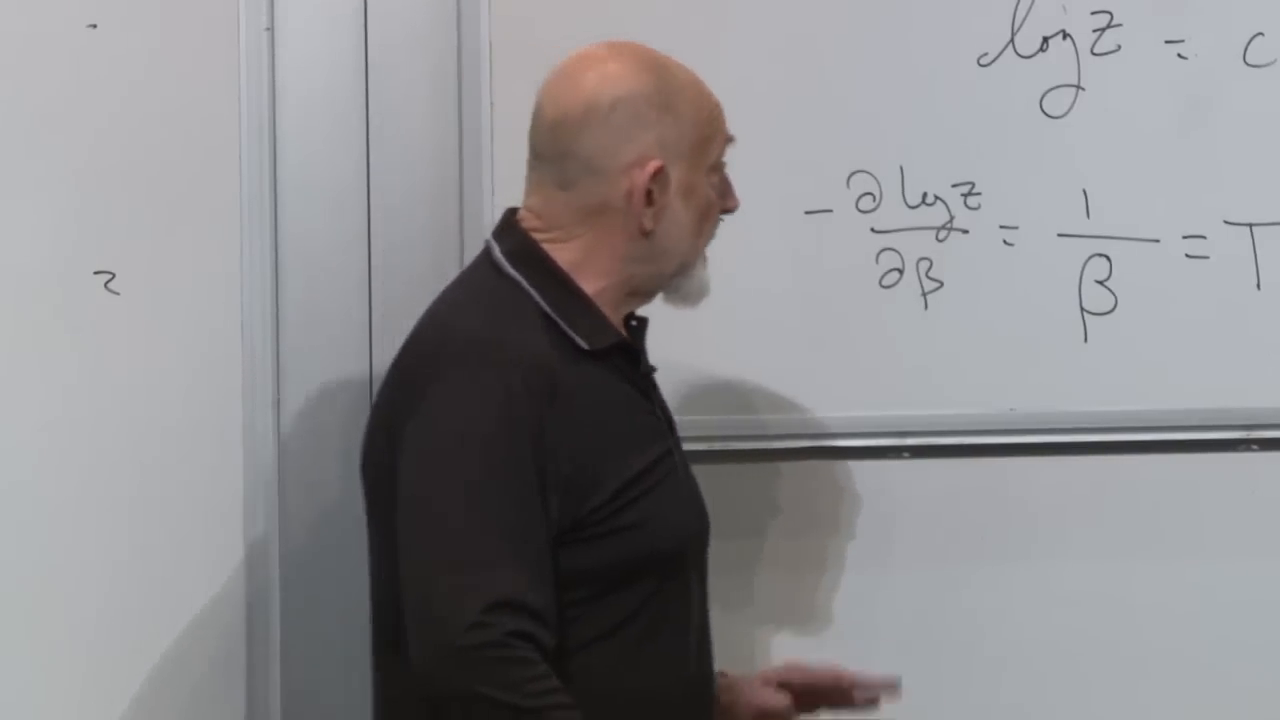
\includegraphics[width=0.90\textwidth]{lecture_07_figure_02.png}
\caption{合併展示分子速度的估算、壓力導數及理想氣體代入結果。}
\lectureframe{00:08:55}
\end{figure}

這裡還需要一項重要修正。小振幅聲波造成氣體壓縮與膨脹的速度，通常快於熱量在相鄰氣體微元之間傳遞的速度。因此，局部運動近似為絕熱，而非等溫：
\begin{equation}
 c_s^2=
 \left(\frac{\partial P}{\partial\rho_m}\right)_S.
 \label{eq:sm7-sound-adiabatic}
\end{equation}
對於絕熱指數為 \(\gamma\) 的理想氣體，
\begin{equation}
 P\rho_m^{-\gamma}=\text{constant},
 \qquad
 c_s^2=\gamma\frac{P}{\rho_m}
       =\gamma\frac{k_B T}{m}.
 \label{eq:sm7-sound-ideal-adiabatic}
\end{equation}
室溫下的雙原子空氣，其 \(\gamma\simeq 7/5\)。因此，定溫計算可作為有用的初步估算，而絕熱導數則給出物理上適用的修正。

採用以下粗略數值：
\begin{equation}
\begin{aligned}
 k_B&\simeq1.3\times10^{-23}\ {\rm J\,K^{-1}},
 &T&\simeq300\ {\rm K},\\
 m_{\rm air}&\simeq4\times10^{-26}\ {\rm kg}.&&
\end{aligned}
 \label{eq:sm7-air-data}
\end{equation}
分子速度估算值約為 \(500\ {\rm m\,s^{-1}}\)。此處的溫度必須是以開爾文表示的絕對溫度，不能使用華氏這類以偏移量為基準的溫標。熟知的聲速約為 \(300\ {\rm m\,s^{-1}}\)；絕熱理想氣體公式則在室溫下給出約 \(340\ {\rm m\,s^{-1}}\)。因此，這項粗略計算得到了正確的物理尺度。

\begin{figure}[t]
\centering
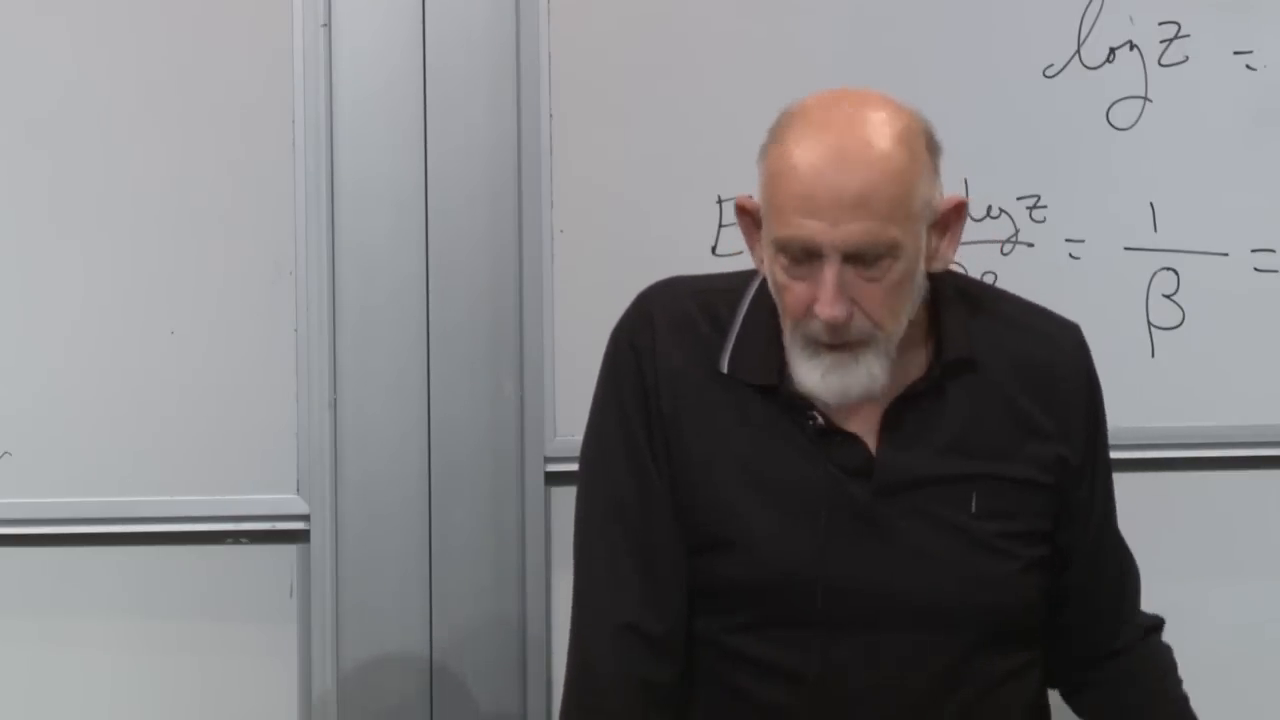
\includegraphics[width=0.90\textwidth]{lecture_07_figure_03.png}
\caption{以玻爾茲曼常數、約為 \(30\) 個質子質量的有效分子質量，以及 \(T\simeq300\ {\rm K}\)，估算室溫空氣中的聲速。}
\lectureframe{00:10:55}
\end{figure}

早在微觀理論尚未出現之前，人們就能藉由測量壓力隨密度的變化來求得聲速。統計力學的論證進一步提供了一個引人注目的解釋：所得的宏觀速度由單一分子的熱運動速度決定。

\begin{classroomqa}
\audiencequestion{分子質量是否應計入中子？氮的數值 \(14\) 是否只計算質子？}
\lecturerresponse{引用的原子量已將質子和中子都計入。氮分子含有兩個原子，每個原子的原子量約為 \(14\)，因此分子質量約為 \(28\) 個質子質量。就這項估算而言，將 \(28\) 約取為 \(30\) 已足夠。
\lecturetimestamp{00:10:58--00:11:16}}
\end{classroomqa}

\begin{classroomqa}
\audiencequestion{因子 \(3\) 來自三個平移方向，但聲波只沿一個方向傳播。這是否表示應該去掉因子 \(3\)？}
\lecturerresponse{這個問題提醒我們，不應把三維的分子均方根速率等同於一維的傳播速率。前面的論證只是數量級估算。要得到受控的結果，應使用壓力導數，並採用適用於該波的熱力學條件。
\lecturetimestamp{00:11:12--00:12:00}}
\end{classroomqa}

\begin{classroomqa}
\audiencequestion{這個導數是否假設波傳播時溫度保持不變？}
\lecturerresponse{是的，展示的理想氣體代入式採用了這項假設。對極小的擾動而言，定溫是合理的初步估算；標準修正則是將一般聲波視為近似絕熱，並以 \(\left(\partial P/\partial\rho_m\right)_S\) 取代等溫導數。
\lecturetimestamp{00:12:59--00:14:01}}
\end{classroomqa}

\begin{classroomqa}
\audiencequestion{如果壓力和密度的變化都很小，它們的導數是否也會很小？}
\lecturerresponse{不會。導數是在無窮小極限下兩個小變化量的比值。\(\delta P\) 和 \(\delta\rho\) 都可能很小，但 \(\delta P/\delta\rho\) 仍可維持有限，並決定波速。
\lecturetimestamp{00:14:03--00:14:23}}
\end{classroomqa}

\begin{classroomqa}
\audiencequestion{氣體受到壓縮時，聲速是否應該提高，就像物質從氣體轉變為液體或固體時那樣？}
\lecturerresponse{是。導數是在所考慮的狀態下計算的，而 \(P(\rho,T)\) 不一定是線性函數。分子被擠得彼此靠近時，狀態方程會偏離理想氣體形式，\(\partial P/\partial\rho\) 也可能大幅增加。
\lecturetimestamp{00:14:25--00:15:13}}
\end{classroomqa}

\begin{classroomqa}
\audiencequestion{數值 \(500\ {\rm m\,s^{-1}}\) 能否用於任意壓力？}
\lecturerresponse{不能。這個數值適用於低密度範圍，因為在此範圍內理想氣體方程是有用的近似。一旦 \(P(\rho,T)\) 中出現密度的高次項，導數因而聲速，就會隨壓力和密度而變化。
\lecturetimestamp{00:15:14--00:16:29}}
\end{classroomqa}

\begin{classroomqa}
\audiencequestion{密度增加時，聲波以約略等於分子速度的速度傳播這個原先的圖像，是否也會失效？}
\lecturerresponse{很可能會。這個圖像是針對稀薄氣體提出的。密度高時，集體交互作用會變得愈來愈重要；這正是狀態方程的導數能提供更一般描述的原因。
\lecturetimestamp{00:16:32--00:16:53}}
\end{classroomqa}

\begin{classroomqa}
\audiencequestion{為什麼氮分子的質量寫成約 \(30\) 個質子質量，而不是 \(28\)？}
\lecturerresponse{這項估算只需要相稱的數值精度，因此將 \(28\) 約取為 \(30\)。原先的 \(500\ {\rm m\,s^{-1}}\) 估算值除以 \(\sqrt{3}\simeq1.7\) 後也接近 \(300\ {\rm m\,s^{-1}}\)，不過要計算修正量，仍應採用絕熱導數這種受控的方法。
\lecturetimestamp{00:16:54--00:17:27}}
\end{classroomqa}

\section{熱浴中的單一經典振子}

現在，我們以單一諧振子取代自由平移的分子，並把其他一切視為熱浴。彈簧上掛著質量塊，是最直接的例子，但這個模型的適用範圍更廣。電磁腔中的模式會振盪；晶體中的原子會振盪；幾乎任何穩定系統只要稍微偏離平衡，在最低階近似下都會作簡諧運動。

令 \(x\) 表示相對於平衡位置的位移，動量為 \(p\)、質量為 \(m\)，彈簧常數為 \(\kappa\)，則哈密頓量為
\begin{equation}
 H(x,p)=\frac{p^2}{2m}+\frac{\kappa x^2}{2},
 \qquad
 \omega=\sqrt{\frac{\kappa}{m}}.
 \label{eq:sm7-classical-hamiltonian}
\end{equation}
熱浴決定 \(T\)；從此處起，我們再次採用 \(k_B=1\)，因此 \(\beta=1/T\)。與室溫環境達到平衡的振子，其溫度約為 \(300\ {\rm K}\)；浸在液態氦中的振子，溫度則只有幾開爾文。假想的彈簧若置於太陽中心，便無法維持彈簧的狀態，但這個例子清楚說明了環境的作用。玻爾茲曼權重可分解為
\begin{equation}
 e^{-\beta H}
 =e^{-\beta p^2/(2m)}
  e^{-\beta\kappa x^2/2}.
 \label{eq:sm7-factorized-weight}
\end{equation}

\begin{figure}[t]
\centering
\includegraphics[width=0.90\textwidth]{lecture_07_figure_04.png}
\caption{彈簧質量振子，以及由動能和位能組成的哈密頓量。}
\lectureframe{00:20:55}
\end{figure}

與自由氣體不同，位置積分不只是給出容器體積。回復力位能會對每個位移加權：
\begin{equation}
 Z_{\rm cl}
 =\frac{1}{h}\int_{-\infty}^{\infty}dp
             \int_{-\infty}^{\infty}dx\,
 e^{-\beta p^2/(2m)}
 e^{-\beta\kappa x^2/2}.
 \label{eq:sm7-classical-z}
\end{equation}
因子 \(1/h\) 使一維經典配分函數成為無因次量。板書計算中省略了這個因子，因為它與 \(\beta\) 無關，也不會影響平均能量。

\begin{figure}[t]
\centering
\includegraphics[width=0.90\textwidth]{lecture_07_figure_05.png}
\caption{經典振子的配分函數分解為動量與位移兩個高斯積分。}
\lectureframe{00:22:55}
\end{figure}

對動量積分，令
\begin{equation}
 q=\sqrt{\frac{\beta}{2m}}\,p,
 \qquad
 dp=\sqrt{\frac{2m}{\beta}}\,dq.
 \label{eq:sm7-p-gaussian-substitution}
\end{equation}
對位置積分，令
\begin{equation}
 y=\sqrt{\frac{\beta\kappa}{2}}\,x,
 \qquad
 dx=\sqrt{\frac{2}{\beta\kappa}}\,dy.
 \label{eq:sm7-x-gaussian-substitution}
\end{equation}
由於 \(\int_{-\infty}^{\infty}e^{-u^2}\,du=\sqrt{\pi}\)，板書中使用的未歸一化相空間積分為
\begin{equation}
 \int dp\,dx\,e^{-\beta H}
 =\frac{2\pi}{\beta}\sqrt{\frac{m}{\kappa}}
 =\frac{2\pi}{\beta\omega}.
 \label{eq:sm7-classical-z-unnormalized}
\end{equation}
恢復相空間胞元後，得到
\begin{equation}
 Z_{\rm cl}=\frac{2\pi}{h\beta\omega}
           =\frac{1}{\beta\hbar\omega}.
 \label{eq:sm7-classical-z-normalized}
\end{equation}

只有對能量有影響的 \(\beta\) 依賴部分：
\begin{equation}
 \begin{aligned}
 \log Z_{\rm cl}&=\text{constant}-\log\beta,\\
 \expect{H}
 &=-\frac{\partial\log Z_{\rm cl}}{\partial\beta}\\
 &=\frac{1}{\beta}=T.
 \end{aligned}
 \label{eq:sm7-classical-energy}
\end{equation}

\begin{figure}[t]
\centering
\includegraphics[width=0.90\textwidth]{lecture_07_figure_06.png}
\caption{右側黑板上的完整經典推導：高斯積分的因式分解、\(Z\propto(\beta\omega)^{-1}\)，以及 \(\expect{H}=1/\beta=T\)。}
\lectureframe{00:30:15}
\end{figure}

這裡沒有因子 \(3\)，因為只有一個空間維度的振子。也沒有剩下因子 \(1/2\)，因為哈密頓量包含兩個獨立的二次項。每個高斯積分都貢獻 \(T/2\)：
\begin{equation}
 \expect{K}=\frac{T}{2},
 \qquad
 \expect{U}=\frac{T}{2},
 \qquad
 \expect{H}=T.
 \label{eq:sm7-equipartition-oscillator}
\end{equation}
這是最實用的能量均分形式：經典哈密頓量中的每個獨立二次項都貢獻 \(T/2\)。

答案與 \(m\) 和 \(\kappa\) 都無關，但運動本身確實取決於這兩個參數：
\begin{equation}
 \expect{p^2}=mT,
 \qquad
 \expect{x^2}=\frac{T}{\kappa},
 \qquad
 \expect{\dot{x}^2}=\frac{T}{m}.
 \label{eq:sm7-classical-fluctuations}
\end{equation}
因此，質量較大的物體運動較慢，彈簧較硬時振幅較小，但平均能量仍為 \(T\)。當 \(\kappa\) 大得驚人時，這個結果便令人不安。硬到幾乎無法運動的彈簧，理應如同凍結的約束；然而經典能量均分定理仍賦予它 \(T\) 的能量。

\begin{classroomqa}
\audiencequestion{當 \(\kappa\to\infty\) 時，配分函數趨近於零。為什麼仍然可以使用它的對數？}
\lecturerresponse{讓 \(\kappa\) 保持有限，但可以任意大。它對 \(\log Z\) 的貢獻是加法項，且與 \(\beta\) 無關，因此對 \(\beta\) 微分仍會得到 \(T\)。這種極限情況帶來的不安確實存在：經典計算本身邏輯一致，但它漏掉了自然界中一項對極硬振子不可或缺的特性。
\lecturetimestamp{00:34:01--00:34:54}}
\end{classroomqa}

\begin{classroomqa}
\audiencequestion{理想氣體的配分函數需要一個 \(N!\)。這裡是否也應該有類似的階乘？}
\lecturerresponse{不需要。我們研究的是一個指定的振子，而不是排列 \(N\) 個全同粒子。若有許多彼此獨立且各自可辨識的模式，配分函數就彼此相乘。不可區分性因子適用於另一種計數問題。
\lecturetimestamp{00:35:03--00:35:40}}
\end{classroomqa}

\section{經典能量均分為何成了一場危機}

真實分子並非沒有結構的點粒子。雙原子分子包含可振動的化學鍵，因此具有內部振子。若按經典理論直接計數，即使在一般溫度下，也會把額外的熱能分配給這個模式。以刻意簡化的示意性計算來說，啟動一個振動模式，會使能量從 \(3T/2\) 提高到接近 \(5T/2\)。若要精確計算熱容量，還必須納入轉動自由度，並區分能量與能量對溫度的導數。更直接的關鍵實驗事實是：低溫下，剛性的內部模式並未如經典能量均分定理所預測的那樣貢獻能量。

一種做法是否認分子具有內部結構，但這顯然荒謬；另一種做法則是承認經典力學缺少了某個要素。這個要素就是量子力學。我們只需要其中很少的一部分：諧振子的能階等間距。

\section{量子振子}

首先移動能量的基準點，將激發能譜寫成
\begin{equation}
 E_n^{\rm exc}=n\hbar\omega,
 \qquad n=0,1,2,\ldots.
 \label{eq:sm7-shifted-spectrum}
\end{equation}
此時的配分函數是真正的求和，而不是相空間積分：
\begin{align}
 Z_{\rm exc}
 &=\sum_{n=0}^{\infty}e^{-\beta n\hbar\omega} \notag\\
 &=1+x+x^2+\cdots
  =\frac{1}{1-x},
 \qquad x=e^{-\beta\hbar\omega}, \notag\\
 &=\frac{1}{1-e^{-\beta\hbar\omega}}.
 \label{eq:sm7-quantum-z}
\end{align}

\begin{figure}[t]
\centering
\includegraphics[width=0.90\textwidth]{lecture_07_figure_07.png}
\caption{等間距能階，以及利用幾何級數計算量子振子的配分函數。}
\lectureframe{00:42:05}
\end{figure}

微分後得到平均激發能：
\begin{align}
 E_{\rm exc}
 &=-\frac{\partial\log Z_{\rm exc}}{\partial\beta}
  =-\frac{1}{Z_{\rm exc}}
    \frac{\partial Z_{\rm exc}}{\partial\beta}
 \notag\\
 &=\hbar\omega\,
   \frac{e^{-\beta\hbar\omega}}
        {1-e^{-\beta\hbar\omega}}
  =\frac{\hbar\omega}{e^{\beta\hbar\omega}-1}.
 \label{eq:sm7-quantum-energy}
\end{align}

\begin{figure}[t]
\centering
\includegraphics[width=0.90\textwidth]{lecture_07_figure_08.png}
\caption{量子配分函數對 \(\beta\) 微分後所得的熱激發能。}
\lectureframe{00:46:05}
\end{figure}

\subsection{高溫}

當 \(\beta\hbar\omega\ll1\) 時，
\begin{equation}
 e^{-\beta\hbar\omega}
 =1-\beta\hbar\omega
  +O\!\left((\beta\hbar\omega)^2\right).
 \label{eq:sm7-high-t-expansion}
\end{equation}
\eqref{eq:sm7-quantum-energy} 的分子趨近 \(\hbar\omega\)，而分母在最低階近似下為 \(\beta\hbar\omega\)。因此
\begin{equation}
 E_{\rm exc}\simeq\frac{1}{\beta}=T.
 \label{eq:sm7-high-t-energy}
\end{equation}
當熱能涵蓋許多能階間距時，量子力學的結果便回復為經典能量均分定理。

\subsection{低溫}

當 \(\beta\hbar\omega\gg1\) 時，指數項非常小：
\begin{equation}
 E_{\rm exc}
 \simeq\hbar\omega e^{-\beta\hbar\omega}.
 \label{eq:sm7-low-t-energy}
\end{equation}
振子的熱激發受到指數抑制。在平移後的能量基準下，激發能幾乎為零；稍後會再把物理上的零點能加回來。

\begin{figure}[t]
\centering
\includegraphics[width=0.90\textwidth]{lecture_07_figure_09.png}
\caption{低溫展開：第一個熱激發受到 \(e^{-\beta\hbar\omega}\) 抑制。}
\lectureframe{00:51:55}
\end{figure}

交越發生在
\begin{equation}
 \beta\hbar\omega\sim1,
 \qquad\text{or equivalently}\qquad
 T\sim\hbar\omega.
 \label{eq:sm7-crossover}
\end{equation}
這個條件有直接的物理意義。經典能量均分定理會給振子 \(T\) 的能量。當這個尺度低於一個能階間距時，量子效應便不可忽略。因此
\begin{equation}
\begin{aligned}
 \hbar\omega\gg T&:\quad \text{frozen and quantum},\\
 \hbar\omega\ll T&:\quad \text{active and classical}.
\end{aligned}
 \label{eq:sm7-regimes}
\end{equation}
較硬的彈簧具有較大的 \(\omega=\sqrt{\kappa/m}\)，所以需要較高的溫度，振子才會呈現經典行為。

\section{加熱物質時，自由度逐漸顯現}

低溫時，雙原子分子的剛性鍵結振動處於凍結狀態，因此在熱學上可能近似點粒子。當 \(T\) 升高到超過 \(\hbar\omega\) 時，振動模式便會啟動。轉動模式可能在較低的能量尺度就會啟動；溫度再升高，會顯現更多內部運動，最後甚至使原子電離。加熱不只是把更多能量注入一份固定的模式清單；它也會揭露低溫時不可見的自由度。

假想的巢狀分子能更清楚地說明這一點。兩個原子由一根剛性彈簧連接，其中一個表面上看似單一原子的部分，其實又是由更硬的彈簧連接的一對原子。在低 \(T\) 時，兩種結構看起來都像點粒子。達到第一個閾值時，外層振動模式出現；達到第二個閾值時，內部結構才顯現。系統的複雜性會隨著能量尺度逐步展開。

\begin{classroomqa}
\audiencequestion{振子進入經典區域後，繼續加熱會使彈簧變緊或改變其頻率嗎？}
\lecturerresponse{不會。彈簧常數和頻率都維持不變。溫度升高會使典型動量和振幅增大，因而提高能量。剛度決定經典定律開始適用的溫度，不代表彈簧會隨溫度升高而變緊。
\lecturetimestamp{01:03:17--01:05:11}}
\end{classroomqa}

\subsection{晶體與愛因斯坦的比熱理論}

晶體包含大量振動模式。經典能量均分定理會為每個活躍振子分配 \(T\) 量級的能量，因此高估低溫下的熱容量。愛因斯坦在 1907 提出的模型以量子力學處理晶體振動，並說明在熱能達到能階間距之前，振動為何受到抑制。更精確的固態模型會納入各模式頻率的分布，但愛因斯坦的計算已經呈現了凍結原理。

\begin{classroomqa}
\audiencequestion{愛因斯坦獲得諾貝爾獎，是因為這項研究嗎？這項研究是否是在量子力學建立後才提出的？}
\lecturerresponse{不是。諾貝爾獎的授獎理由是光電效應。比熱模型於 1907 發表，當時量子力學的完整基礎還遠未建立。愛因斯坦接納並發展了重要的量子觀念，儘管他後來反對成熟量子理論的某些部分。
\lecturetimestamp{00:58:38--01:03:16}}
\end{classroomqa}

\begin{classroomqa}
\audiencequestion{經典統計力學以對位置和動量的表面連續積分，取代對離散狀態的求和。這種狀態計數有什麼根據？}
\lecturerresponse{根本的依據來自量子力學。在高溫極限下，
\[
 Z_{\rm exc}\simeq\frac{1}{\beta\hbar\omega},
\]
這恰好符合無因次的經典結果 \eqref{eq:sm7-classical-z-normalized}。當能階間距無法分辨時，相空間中的量子胞元便會導出經典的相空間測度。
\lecturetimestamp{00:59:38--01:03:06}}
\end{classroomqa}

\subsection{一條弦包含無窮多個振子}

小提琴弦或吉他弦可以分解為正規模式：基頻、高次諧波，以及波長愈來愈短的模式。從數學上看，這些振子模式有無窮多個。若經典能量均分定理為每個模式分配 \(T\) 的能量，處於熱平衡的弦便會具有無窮大的能量。量子力學避免了這個災難。波長最短的模式頻率最高，在任何有限溫度下都維持凍結；隨著 \(T\) 升高，啟動的模式也愈來愈多。稍後討論黑體輻射時，也會用到相同的道理。

\begin{figure}[t]
\centering
\includegraphics[width=0.90\textwidth]{lecture_07_figure_10.png}
\caption{弦上數個正規模式的疊加，說明連續弦為何相當於無窮多個諧振子的集合。}
\lectureframe{01:09:30}
\end{figure}

\begin{classroomqa}
\audiencequestion{量子到經典的交越能直接觀察到嗎？加熱能否使低溫時的行為逆轉？}
\lecturerresponse{可以。晶體比熱隨溫度的變化，能清楚測出振動模式的凍結及其後的逐步啟動。
\lecturetimestamp{01:09:11--01:10:13}}
\end{classroomqa}

\begin{classroomqa}
\audiencequestion{對於多個振子，是否要為每個模式各自使用單一振子的配分函數？}
\lecturerresponse{對於彼此獨立的模式，
\[
\begin{aligned}
 Z_{\rm tot}&=\prod_j Z_j,&
 \log Z_{\rm tot}&=\sum_j\log Z_j,\\
 E_{\rm tot}&=\sum_j E_j.&&
\end{aligned}
\]
若 \(\hbar\omega_j\gg T\)，模式對熱能的貢獻便會小到呈指數抑制；低於這個閾值的模式則會有顯著貢獻。
\lecturetimestamp{01:10:14--01:11:00}}
\end{classroomqa}

\begin{classroomqa}
\audiencequestion{振子的零點能 \(\hbar\omega/2\) 到哪裡去了？}
\lecturerresponse{物理能階為
\[
 E_n=\left(n+\frac12\right)\hbar\omega.
\]
因此
\[
 \begin{aligned}
 Z_{\rm phys}
 &=e^{-\beta\hbar\omega/2}Z_{\rm exc},\\
 E_{\rm phys}
 &=\frac{\hbar\omega}{2}
  +\frac{\hbar\omega}{e^{\beta\hbar\omega}-1}.
 \end{aligned}
\]
這個共同的能量位移不會改變能階機率、熵、熱容量或熱激發能，但會使絕對平均能量增加 \(\hbar\omega/2\)。\(Z\) 中的乘法因子取決於 \(\beta\)；若要求絕對能量，就不能把它省略。
\lecturetimestamp{01:11:08--01:11:37}}
\end{classroomqa}

\section{第二定律的可逆性謎題}

現在可以回到先前提過的問題。第二定律指出，一般的宏觀演化具有不可逆性，而且熵傾向於增加。微觀的哈密頓演化卻是可逆的。對精確狀態進行的可逆映射，如何能產生描述宏觀狀態的不可逆定律？

以高維相空間中的一個點表示系統：
\[
 \Gamma=(q_1,\ldots,q_N,p_1,\ldots,p_N).
\]
我們掌握的資訊通常不足以把狀態確定為一個精確的點。假設機率密度在一個緊緻區域 \(A\) 內均勻分布，該區域的體積為 \(\Omega_A\)：
\begin{equation}
 f(\Gamma)=
 \begin{cases}
  1/\Omega_A,&\Gamma\in A,\\
  0,&\Gamma\notin A.
 \end{cases}
 \label{eq:sm7-uniform-blob}
\end{equation}
在 \(k_B=1\) 的單位制下，細粒化的吉布斯熵為
\begin{equation}
 S_{\rm fine}
 =-\int d\Gamma\,f\log f
 =\log\Omega_A.
 \label{eq:sm7-blob-entropy}
\end{equation}
區域愈小，代表資訊愈多、熵愈低。這也確定了符號方向：不確定性增加會使佔據區域擴大，並提高 \(\log\Omega_A\)。

\begin{figure}[t]
\centering
\includegraphics[width=0.90\textwidth]{lecture_07_figure_11.png}
\caption{完整位置—動量相空間的一個示意性二維切面，其中有一個緊緻的機率分布區域。}
\lectureframe{01:20:20}
\end{figure}

\begin{classroomqa}
\audiencequestion{系統是否受物理限制，必須留在圖中所畫的區域內？它是否已經處於平衡狀態？}
\lecturerresponse{不是。這個區域表示我們對初始狀態的認識，而不是相空間中的一道牆。系統也不一定已處於平衡狀態。舉例來說，氣體最初被限制在房間一角的容器中，就是一種特殊的非平衡初始資訊。
\lecturetimestamp{01:14:55--01:15:24}}
\end{classroomqa}

\section{劉維爾流與粗粒化區域的擴大}

劉維爾定理指出，哈密頓流會保持相空間體積不變。精確區域可以平移、拉伸、摺疊並變得極其細長，但
\begin{equation}
 \Omega_{A(t)}=\Omega_{A(0)},
 \qquad
 S_{\rm fine}(t)=S_{\rm fine}(0).
 \label{eq:sm7-liouville}
\end{equation}
離散系統中的類比，是狀態的可逆排列。若一開始知道骰子處於兩種狀態之一，一對一的演化可以改變是哪兩種狀態，卻不會改變可能狀態的數目。

實際描述的解析度有限。量子力學提供了自然的相空間胞元；即使不援引量子理論，經典實驗的測量能力也有限。在哈密頓流下，分布區域可能變成一條細長的蛇。若相鄰蛇身摺層間的距離小於解析度，我們便以粗粒化胞元取代每個無法分辨的區域。精確的佔據體積維持不變，但粗粒化胞元的聯集會擴大：
\begin{equation}
 \Omega_{\rm coarse}(t)\geq\Omega_{A(t)},
 \qquad
 S_{\rm coarse}(t)=\log\Omega_{\rm coarse}(t).
 \label{eq:sm7-coarse-entropy}
\end{equation}

\begin{figure}[t]
\centering
\includegraphics[width=0.90\textwidth]{lecture_07_figure_12.png}
\caption{以有限解析度的胞元觀察一條保持體積的細絲。精確的黑色細絲面積不變；紅色粗粒化胞元所占的有效區域則更大。}
\lectureframe{01:22:10}
\end{figure}

\begin{classroomqa}
\audiencequestion{粗粒化胞元彼此重疊。這是否違反劉維爾定理？}
\lecturerresponse{不會。劉維爾定理適用於精確的細絲；細絲仍保持一對一映射和體積不變。重疊只出現在模糊化的描述中：我們已捨棄了狀態位於哪一條細絲分支上的資訊。
\lecturetimestamp{01:21:32--01:21:50}}
\end{classroomqa}

棉絮是個有用的類比。所有纖維的材料體積幾乎可以保持不變，但對於無法分辨單根纖維的觀察者而言，一團被拉鬆的棉絮看起來會占據很大的體積。同樣地，相空間中的區域會伸出愈來愈細的觸鬚，這些觸鬚又會分出更細的觸鬚。任何固定的有限解析度，最終都無法追蹤它們。

\begin{classroomqa}
\audiencequestion{熵在經典描述中是否只是看似增加？量子力學是否透過設定基本解析度極限，才使熵增加成為真實現象？}
\lecturerresponse{粗粒化的論證不需要量子力學設定的極限。熵同時涉及系統本身，以及描述中保留的宏觀區別。若掌握無限的微觀資訊，細粒化熵便維持不變；若解析度固定且有限，混沌形成的細絲最終會變得無法分辨，粗粒化熵便會增加。
\lecturetimestamp{01:24:04--01:25:20}}
\end{classroomqa}

\section{混沌、有限的可達區域與平衡化}

在盒中的氣體，粒子位置受到限制。在總能量固定且有限時，動量也有界，即使全部能量暫時集中在一個粒子上也是如此。因此，在通常的束縛假設下，動力學上可達的能量殼層具有有限測度。

\begin{figure}[t]
\centering
\includegraphics[width=0.90\textwidth]{lecture_07_figure_13.png}
\caption{有限的可達相空間區域，旁邊示出細絲及其粗粒化表示。}
\lectureframe{01:28:10}
\end{figure}

混沌系統中，彼此接近的初始點會在一段時間內沿著相似的歷程演化，之後才逐漸分離。在一次撞球開球中，母球方向上微不可察的變化會一路傳遞到後續碰撞；差異不斷累積，直到最終構型彼此毫不相關。因此，整個初始區域會在可及區域中被拉伸、摺疊。在有限解析度下，它會逐漸呈現範圍廣大、近乎均勻的平衡描述。

\begin{figure}[t]
\centering
\includegraphics[width=0.90\textwidth]{lecture_07_figure_14.png}
\caption{一個緊緻的特殊態在有界的可及區域中演化成複雜的細絲，而粗粒化元胞則擴散至大得多的面積。}
\lectureframe{01:33:10}
\end{figure}

有兩點需要限定。混沌本身並不能證明每條軌跡都會造訪每個可及鄰域；要提出更強的遍歷主張，還需要遍歷性或混合性質。物理系統也不全是混沌的。一般的多體氣體和理想化的撞球系統，是這裡所要討論的情境；在這些情境中，混合是有用的物理預期。

\section{迴歸不會消除不可逆性}

假設所有空氣分子一開始都位於房間的一個角落，而且具有特別製備的速度分布。碰撞很快就會使它們散布到整個房間，粗粒化描述也會達到平衡。在有限且保測度的相空間中，龐加萊迴歸定理指出，幾乎所有初始點都會再次任意接近起點。對於容差 \(\epsilon>0\)，在定理的假設下，迴歸時間 \(t_R(\epsilon)\)是有限的；然而，對宏觀系統而言，這段時間大得驚人。無須、通常也不預期系統會精確回到一個精度無限的點。

\begin{classroomqa}
\audiencequestion{在撞球的例子中，擊打母球會不會注入能量，因而破壞封閉系統的演化？}
\lecturerresponse{所選的初始態是從擊球之後立即開始的，因此擊球所給予的能量已包含在內。迴歸所涉及的是此後孤立的理想化撞球系統動力學；回到初始態附近，意味著母球會在所選容差範圍內接近球組。
\lecturetimestamp{01:35:37--01:35:55}}
\end{classroomqa}

\begin{classroomqa}
\audiencequestion{如果氣體最終可能回到角落，我們是否就失去了資訊？系統真的可逆嗎？}
\lecturerresponse{微觀動力學始終保持可逆。粗粒化熵可以上升，因為我們不再解析精細的關聯；然而，極其罕見的漲落仍可能使系統回到接近其特殊初始宏觀態的狀態。因此，迴歸與粗粒化不可逆性彼此相容。
\lecturetimestamp{01:37:34--01:38:15}}
\end{classroomqa}

這引出玻爾茲曼的核心表述。熵並非在邏輯上可能的每一個瞬間都會增加。對於一個大型系統的非平衡宏觀態，與之相容的微觀演化中，通往較大宏觀態的情形遠多於通往更特殊宏觀態的情形。熵 \emph{很可能}增加。向下漲落和迴歸都是可能的，但其機率和時間尺度使它們在一般的宏觀經驗中無從察覺。可逆性問題是統計力學史上重大的爭論之一，也令玻爾茲曼深受困擾。但不應因此對他的一生作出簡單的因果推論。

\section{混沌的意義}

若要更具體地定義混沌，假設兩個初始相點相差 \(\delta\Gamma(0)\)。在線性化近似仍適用的區域內，沿著混沌方向的分離通常符合
\begin{equation}
 \lVert\delta\Gamma(t)\rVert
 \sim e^{\lambda t}\lVert\delta\Gamma(0)\rVert,
 \qquad \lambda>0,
 \label{eq:sm7-lyapunov-growth}
\end{equation}
數值 \(\lambda\)稱為李雅普諾夫指數。若要預測時間 \(t\)之後的狀態，初始資料所需的精度大致按 \(e^{-\lambda t}\)縮放。動力學定律的精度也很重要：模型誤差也會和初始條件的誤差一樣受到放大。天氣就是一個熟悉的例子。

\begin{classroomqa}
\audiencequestion{有沒有原理能說明 \emph{大多數}系統都是混沌的？還是這只是一種經驗觀察？}
\lecturerresponse{混沌和非混沌的哈密頓量都有無窮多個；甚至「\emph{大多數}」一詞，也需要先在哈密頓量空間上定義測度。複雜的交互作用系統往往是混沌的，但沒有簡單而普遍的檢驗方法，能僅憑檢視就將每個哈密頓量分類。
\lecturetimestamp{01:39:27--01:40:49}}
\end{classroomqa}

\begin{classroomqa}
\audiencequestion{這裡所說的\emph{混沌}，確切來說是什麼意思？}
\lecturerresponse{鄰近的相軌跡分離得足夠快，以致長時間預測需要以指數方式提高對初始條件的掌握精度。諧振子則形成對照：相鄰的相點一同旋轉，彼此始終接近。精確的二體開普勒問題也不是混沌系統，而一般的三體問題則存在混沌區域。
\lecturetimestamp{01:40:50--01:43:45}}
\end{classroomqa}

\begin{classroomqa}
\audiencequestion{運動定律和初始條件都必須掌握得很精確嗎？}
\lecturerresponse{是的。這兩種誤差都會在動力學演化中傳遞，而混沌演化會將兩者都放大。
\lecturetimestamp{01:43:46--01:43:55}}
\end{classroomqa}

雙擺提供了一個生動的例子。單擺是可積且可預測的；加入第二個擺之後，起初幾乎重合的軌跡，最終可能以不同方式傳遞能量，並朝截然不同的方向演化。

\begin{figure}[t]
\centering
\includegraphics[width=0.90\textwidth]{lecture_07_figure_15.png}
\caption{雙擺是確定性混沌的具體例子。}
\lectureframe{01:44:40}
\end{figure}

\begin{classroomqa}
\audiencequestion{為什麼一種力學系統會是混沌的，另一種卻不是？}
\lecturerresponse{這取決於哈密頓量及其不變結構，而不是摩擦或實驗雜訊所致。判定系統是否混沌，在數學上可能很困難；複雜性或許提供線索，但並非證明。
\lecturetimestamp{01:44:03--01:45:58}}
\end{classroomqa}

\begin{classroomqa}
\audiencequestion{理想的雙擺即使沒有摩擦，仍然會是混沌系統嗎？}
\lecturerresponse{是的，不需要耗散。精確的確定性哈密頓運動也可能對初始條件具有敏感依賴性。若初始資料的精度無限，軌跡就能無限期地確定；但精度有限，預測時限也有限。
\lecturetimestamp{01:45:57--01:47:54}}
\end{classroomqa}

\begin{classroomqa}
\audiencequestion{混沌是否等同於沒有閉式解？}
\lecturerresponse{不是。混沌系統通常沒有全域適用且實用的閉式軌跡解，但解析可解性和敏感依賴性是不同的性質。混沌是根據軌跡的分離情形，從動力學上加以判定，而不只是因為我們寫不出公式。
\lecturetimestamp{01:48:20--01:49:23}}
\end{classroomqa}

\begin{classroomqa}
\audiencequestion{普遍存在的混沌，和恰好平衡在不穩定的山頂上有何不同？}
\lecturerresponse{山頂是個特殊的不穩定狀態：離開山頂後，鄰近軌跡未必會迅速分離。在混沌區域中，沿著軌道，不穩定性是常見的；鄰近相點也會反覆分離。正的李雅普諾夫指數刻畫了這種持續增長。
\lecturetimestamp{01:49:27--01:50:11}}
\end{classroomqa}

\section{從微觀運動到統計定律}

聲速估算顯示，微觀熱運動如何決定宏觀的傳播尺度；課堂上的提問則指出，必須指定哪一個熱力學導數。接著，振子展現了經典能量均分定理的適用範圍及其失效。量子能級間距會使高剛性模態凍結，解釋熱容量為何隨溫度改變，也避免無窮多個高頻模態承載無窮大的熱能。

從精確的微觀物理到有效的宏觀描述，這條脈絡也化解了第二定律核心處看似矛盾之處。哈密頓流保持精確的相空間體積不變，也維持可逆性。混沌拉伸會產生比宏觀描述所能保留的更細緻的關聯，因此粗粒化後的佔據區域會擴大。迴歸定理保證罕見的返回並非不可能；機率則解釋了為什麼這類返回不會出現在日常經驗中。第二定律並非新的不可逆微觀力，而是具有極多自由度的系統在特殊宏觀初始條件下，演化方向極為可靠的統計趨勢。
\chapter{復現、非平衡有序與伊辛自旋}

\lectureoverview{從房間一半釋出的氣體會迅速趨近平衡，但可逆力學指出，演化時間足夠長時，系統也必定會返回那個特殊狀態。我們根據相空間體積估算復現時間，區分復現與宇宙低熵起始狀態之謎，並藉此討論玻爾茲曼大腦、彼此連貫的歷史，以及由能量流維持的生命。接著我們轉向磁有序。彼此獨立的兩態自旋提供了一個可精確求解的入門例子：組合計數決定配分函數，而磁化強度呈雙曲正切函數的形式。加入近鄰相互作用後，上--下對稱性便得以恢復，並導向一維伊辛模型。}

\section{一屋子的空氣終將復現}

先讓房間裡的空氣全都位於左半邊。可以用隔板製備這個狀態：將右半邊抽成真空，把空氣留在左半邊，然後移除隔板。氣體迅速擴散至整個房間，並趨近熱平衡。熵增加了。沒有什麼令人意外之處。

現在將房間密封起來，等待下去。連續擲出一百萬次正面的紀錄極不可能發生，但若無限次重複實驗，終究會出現極不可能的紀錄。氣體也是同樣的道理。在某個遙遠的時刻，所有分子會再次出現在左半邊，或某個同樣特殊的區域。這種返回稱為龐加萊復現。

精確的定理比這幅圖像所呈現的情況稍微嚴謹一些。對於相空間中一個測度有限、且動力學保持相空間體積不變的區域，幾乎所有初始點都會任意接近原來的起點。像\emph{所有分子都在左半邊}這樣的宏觀敘述比較容易成立：它只要求軌跡重新進入一個有限的粗粒化區域，不要求每個分子座標都精確地回到原值。實際上要問的是，這需要多久。

\subsection{高維相點}

對\(N\)個經典粒子而言，相空間有\(6N\)個座標，\begin{equation}
 \Gamma=(\bm x_1,\ldots,\bm x_N;\bm p_1,\ldots,\bm p_N).
 \label{eq:sm8-phase-point}
\end{equation}位置受房間範圍限制。在總能量固定時，動量也有界，因為單一粒子若帶有任意大的動量，就必須具有任意大的能量。因此，在復現論證所採用的假設下，允許的能量殼具有有限測度。

相點按照確定性規律演化，但多體氣體中的運動具有混沌性。相鄰軌跡會迅速分離，就像一連串撞球碰撞一樣。經過粗粒化後，漫長軌跡看起來會在可及區域內四處漫遊。

\begin{figure}[t]
\centering
\includegraphics[width=0.90\textwidth]{lecture_08_figure_02.png}
\caption{相空間區域與在其中曲折漫遊的軌跡示意圖。圖中特意只畫出低維情形；真實氣體所在的是\(6N\)維空間。}
\lectureframe{00:06:41}
\end{figure}

這幅低維草圖很容易讓我們立刻犯錯。如果特殊狀態佔據圖中矩形的一半，人們可能會說氣體應有一半時間待在那裡。但\emph{每個分子都位於左半邊}這個條件限制的是每一個位置座標，不只是相點的一個座標。

只考慮在一維空間中運動的兩個粒子，座標為\(x_1\)和\(x_2\)。它們的位形空間是一個正方形。要求\(x_1<L/2\)會選出正方形的一半；若同時要求\(x_1<L/2\)和\(x_2<L/2\)，則會選出四分之一：
\begin{equation}
 P_2=\frac{1}{2}\frac{1}{2}=\frac{1}{4}.
 \label{eq:sm8-two-particle-quarter}
\end{equation}

\begin{figure}[t]
\centering
\includegraphics[width=0.90\textwidth]{lecture_08_figure_07.png}
\caption{對於兩個一維粒子，較小的正方形代表兩個座標都落在房間所選那一半範圍內的組態。}
\lectureframe{00:07:08}
\end{figure}

三個粒子的情況給出\(1/2^3\)，而\(N\)個粒子的情況給出
\begin{equation}
 P_{\mathrm{half}}(N)
 =\left(\frac{1}{2}\right)^N.
 \label{eq:sm8-half-probability}
\end{equation}
指數才是關鍵。二分之一這個因子很平常；但把二分之一提升到巨觀粒子數的次方，就超出了日常直覺。

\begin{classroomqa}
\audiencequestion{答案不應該是\(1/3^N\)嗎？畢竟分子還有其他空間方向。}
\lecturerresponse{這取決於施加的條件。如果只問每個粒子是否都在分隔牆左側，那麼每個粒子只須符合一個二元條件，答案就是\(2^{-N}\)。若再限制粒子只能位於其可用位置空間中另一個獨立的部分，就會再多出一個因子。
\lecturetimestamp{00:07:47--00:08:05}}
\end{classroomqa}

\section{相體積、熵與復現尺度}

同樣的估算也可以不提「一半」來表示。令房間的普通空間體積為\(V\)，並令\(v\)為一個較小的區域，要求所有分子都位於其中。忽略兩種宏觀態共有的動量因子後，可用的位形空間體積為
\begin{equation}
 \Omega_{\mathrm{room}}\propto V^N,
 \qquad
 \Omega_{\mathrm{small}}\propto v^N.
 \label{eq:sm8-config-volumes}
\end{equation}
因此，長時間內處於小區域宏觀態的比例為
\begin{equation}
 P(v)
 =\frac{\Omega_{\mathrm{small}}}{\Omega_{\mathrm{room}}}
 =\left(\frac{v}{V}\right)^N.
 \label{eq:sm8-volume-ratio}
\end{equation}

\begin{figure}[t]
\centering
\includegraphics[width=0.90\textwidth]{lecture_08_figure_08.png}
\caption{黑板上的一般相體積示意圖：可及區域\(V^N\)內的一個小區域\(v^N\)，兩者的比值為\(v^N/V^N\)。}
\lectureframe{00:10:44}
\end{figure}

在\(k_B=1\)的單位制中，熵是可及相體積的對數。若\(S_A=\log\Omega_A\)是受約束宏觀態的熵，而\(S_{\rm eq}=\log\Omega_{\rm eq}\)是平衡態的熵，則
\begin{equation}
 \begin{aligned}
 P(A)
 &=\frac{\Omega_A}{\Omega_{\rm eq}}\\
 &=\exp\!\left(S_A-S_{\rm eq}\right)\\
 &=e^{-\Delta S},\\
 \Delta S&=S_{\rm eq}-S_A.
 \end{aligned}
 \label{eq:sm8-entropy-probability}
\end{equation}
對於半個房間的條件，\(\Delta S=N\log 2\)，而\eqref{eq:sm8-entropy-probability}恰好化為\(2^{-N}\)。只有在將特殊區域的熵視為固定基準時，簡寫\(P\sim e^{-S_{\rm eq}}\)才合適；具有物理意義的指數是熵差\(\Delta S\)。

\begin{classroomqa}
\audiencequestion{這裡指的是位形空間體積，而非整個相空間的體積嗎？}
\lecturerresponse{就這項比較而言，是的。我們施加的是位置條件，而動量分布維持在相同溫度，因此共同的動量空間因子會相消。一般的復現敘述使用相空間；這裡的特定機率則可由位形空間的體積比算出。
\lecturetimestamp{00:11:21--00:11:40}}
\end{classroomqa}

假設系統經過微觀關聯時間或混合時間\(\tau_{\rm mix}\)後，便不再保有對細微位置的記憶。那麼，機率為\(P(A)\)的稀有區域，大約會在以下時間尺度上被遇到：
\begin{equation}
 \tau_{\rm rec}
 \sim \frac{\tau_{\rm mix}}{P(A)}
 \sim \tau_{\rm mix}e^{\Delta S}.
 \label{eq:sm8-recurrence-time-general}
\end{equation}
對於半個房間的條件，
\begin{equation}
 \tau_{\rm rec}\sim\tau_{\rm mix}2^N.
 \label{eq:sm8-recurrence-time-half}
\end{equation}
講課中採用了一個刻意粗略、以房間大小為基準的估算\(N\sim10^{30}\)，得到這個令人印象深刻的尺度：
\(\tau_{\rm rec}/\tau_{\rm mix}\sim2^{10^{30}}\)。在一般大氣密度下，一個房間裡的分子數更接近\(10^{27}\)；不過，把\(10^{30}\)換成\(10^{27}\)，不會改變任何結論：復現時間仍然遠遠超過宇宙年齡，長到難以想像。

\begin{classroomqa}
\audiencequestion{復現時間用什麼單位表示？若從秒改成小時，或改用極短的時間單位，結論會改變嗎？}
\lecturerresponse{量綱前因子是\(\tau_{\rm mix}\)；巨大的數值則是無量綱比值\(\tau_{\rm rec}/\tau_{\rm mix}\)。從秒改成小時，只是除以一般的換算因子；與\(2^{10^{30}}\)相比，這個因子微不足道。單次造訪角落的持續時間確實取決於分子速率，但這項估算關心的是這種造訪要隔多久才會開始。量子復現定理也存在，不過此處用不著。
\lecturetimestamp{00:17:24--00:19:18}}
\end{classroomqa}

\begin{classroomqa}
\audiencequestion{計算一段任何實驗都不可能等待的時間，目的是什麼？}
\lecturerresponse{這是概念上的問題。它告訴我們，封閉力學系統在哪種意義下仍然可逆。系統幾乎所有時間都在平衡態附近，但時間尺度足夠長時，也會發生朝低熵方向的漲落。因此，第二定律是關於特殊初始條件的壓倒性高機率敘述，而不是禁止反向運動的微觀方程式。
\lecturetimestamp{00:15:12--00:16:35}}
\end{classroomqa}

\section{可逆性與特殊的起始狀態}

有意讓系統一開始就處於那個小小的半房間區域。幾乎所有鄰近軌跡都會立刻離開，因為外部的相體積遠大於內部。氣體迅速擴散，接著要等極長時間才會返回。快速弛豫與漫長等待之間的這種不對稱，並不違反可逆力學。

快速逃離過程的時間反演，並不是整段等待時間，而是那段短暫、協調得不可思議的過程：看似處於平衡態的分子速度恰巧以恰當方式排列，使氣體\emph{呼地}衝進房間的一半。若在一般逃離過程結束時反轉每個動量，氣體就會沿原路反向重演逃離過程。漫長的等待時間，指的是那種特殊的入射速度排列自發出現所需的時間。

\begin{classroomqa}
\audiencequestion{時間對稱是否表示緩慢復現到角落所需的時間，會和最初離開角落所需的時間一樣長？}
\lecturerresponse{不會。請比較逃離過程及其精確的時間反演：兩者都很快。漫長的時間花在平衡態中的等待，等待那種觸發反向衝入過程的精確入射漲落。在極其漫長的紀錄中，系統沿兩個時間方向偏離平衡時，局部歷史是對稱的。
\lecturetimestamp{00:20:46--00:21:58}}
\end{classroomqa}

因此，復現論證只能解釋時間箭頭的一部分。它解釋的是：\emph{已知}系統起始於低熵區域時，熵為何通常會上升。它沒有解釋初始條件為何如此特殊。在宇宙學中，這個尚未解答的前提成了核心問題：為什麼可觀測宇宙起始於引力相空間中如此異常狹小的一個區域？

\begin{classroomqa}
\audiencequestion{復現適用於宇宙學嗎？宇宙膨脹開來之後，若等待足夠長的時間，它會復現嗎？}
\lecturerresponse{這個問題無法迴避，但答案取決於整體宇宙學。一個真正封閉且平衡態空間有限的系統，會讓人預期發生復現。膨脹時空、引力、視界，以及無限或非定常的狀態空間，都可能改變論證前提。這裡要強調的教訓較為有限：光靠平衡態復現圖像，並不足以為我們所見這個有結構的宇宙提供令人滿意的統計解釋。
\lecturetimestamp{00:19:59--00:20:45}}
\end{classroomqa}

\begin{classroomqa}
\audiencequestion{復現是否取決於一開始將氣體置於小區域中？若房間一開始就在平衡態，空氣最終還是會聚集到某個角落嗎？}
\lecturerresponse{會。復現關乎封閉系統的長時間動力學，因此，即使初始狀態看似處於平衡，也會發生罕見的低熵漲落。製備半個房間的狀態之所以重要，是另一個原因：這讓我們能以已知的特殊初始狀態為條件，進而追問熵為何在其後立即上升。
\lecturetimestamp{00:22:04--00:22:20}}
\end{classroomqa}

\section{隨機漲落為何預言得太少}

我們或許會想據此建立一套宇宙學：宇宙可能幾乎永遠都處於平衡態，而我們現在的世界只是一次罕見漲落。這個提議過不了一項明確的統計檢驗。以觀察者存在為條件，並問這位觀察者還應預期看到什麼。

足以形成一顆行星的漲落極其罕見。若要形成兩顆行星，就需要更大的熵差，因此更為罕見。若要形成恆星、星系、宇宙微波背景，以及彼此吻合、共同記錄漫長過去的紀錄，則罕見程度還會再多出一個巨大的指數因子。因此，平衡態漲落理論預言的是足以產生觀察者的最小漲落，而不是我們實際觀察到的豐富且彼此連貫的世界。在最極端的情況下，這種最小觀察者稱為玻爾茲曼大腦。

這裡的邏輯是條件機率。令\(A\)表示發生一次觀察者尺度漲落的事件，令\(B\)表示另一個獨立結構。如果兩者各自發生的機率都是很小的\(p\)，那麼
\begin{equation}
 P(B\mid A)=p,
 \qquad
 P(A\cap B)=p^2.
 \label{eq:sm8-conditional-fluctuations}
\end{equation}
得知第一次漲落已經發生，不會讓第二次變得可能。就這個層面而言，彩券的比喻完全貼切：先前的中獎者在下一次獨立抽獎時，並不會有更高的中獎機會。因此，觀察者可以自身存在為條件，但若發現身處的環境另有獨立形成的結構，仍應感到驚訝。

\begin{classroomqa}
\audiencequestion{既然一顆行星或一位玻爾茲曼觀察者已經存在，另一個出現的機率真的比較低嗎？}
\lecturerresponse{第二次獨立罕見漲落的條件機率，仍是單次事件的那個小機率，而不是它的平方；兩者同時發生的聯合機率才是平方。這正是為什麼第一位觀察者仍應預期自身之外是一片熱無序。若發現配偶、另一顆行星和有序的天空，就表示「這位觀察者是由一次孤立的平衡態漲落組成」這個前提不太可能成立。
\lecturetimestamp{00:26:12--00:30:27}}
\end{classroomqa}

\subsection{關於過去的連貫紀錄}

同樣的論證也適用於歷史。彼此一致的兩本教科書、符合同一宇宙膨脹歷史的天文紀錄、地質地層、記憶和實驗室筆記，都會互相約束。一本隨機生成的教科書可以記載任何故事；一整套彼此吻合、共同指向同一段過去的紀錄網絡，所占的相空間區域則小得多。

課堂上的例子提到一個大家熟悉的故事：喬治·華盛頓砍倒了一棵櫻桃樹。這個故事是否屬實並不重要。重點是，若世界是在當下這一刻因漲落而出現，一本書中的句子便沒有任何動力學上的理由，能讓另一筆紀錄與之吻合。彼此連貫的關聯是共同歷史的證據，而非僅僅一次瞬間意外的證據。

\begin{classroomqa}
\audiencequestion{這裡所說的\emph{歷史連貫性}是什麼意思？}
\lecturerresponse{意思是，許多當下的紀錄都能彼此吻合，並可視為共同過去所造成的結果。漲落可以憑空造出紀錄與記憶，但要造出彼此一致的一整套紀錄網絡，所需的漲落遠大於造出一位最小觀察者所需的漲落。因此，復現理論預言，大多數類似觀察者的漲落都缺乏我們實際發現的那種連貫性。
\lecturetimestamp{00:30:30--00:31:12}}
\end{classroomqa}

\begin{classroomqa}
\audiencequestion{宇宙是否仍可能是封閉系統，只是其平衡化與復現時間極為漫長？}
\lecturerresponse{這種可能性並未消除統計問題。若宇宙有無限漫長的歷史，就會有許多類似觀察者的漲落，其中絕大多數都是最小型的漲落，周遭沒有連貫的歷史。從這類漲落中選出一位觀察者，並不應預期會看到我們所觀察到的事物。因此，宇宙學家認真看待玻爾茲曼大腦問題，將它視為檢驗宇宙學測度與晚期宇宙模型的工具，而不是宣稱已經觀測到復現。
\lecturetimestamp{00:31:13--00:32:42}}
\end{classroomqa}

\section{以流動維持的生命結構}

生命看似帶來相反的難題：生物能長期維持精巧的組織結構，不像短暫的意外漲落。解答在於，第二定律適用於完整的封閉系統。子系統可以降低或維持自身熵，只要環境中的熵增加更多：
\begin{equation}
 \dot S_{\rm total}
 =\dot S_{\rm subsystem}+\dot S_{\rm environment}\geq 0.
 \label{eq:sm8-open-system-second-law}
\end{equation}

地球並未處於熱平衡。在人類的時間尺度上，地球近似定常，但定常不代表靜止。能量持續流經地球。陽光抵達地球，經過許多過程後能量品質降低，最後以較低的有效溫度輻射出去。這種能量流可以在總熵增加的同時，維持局部的組織結構。

水流經管道，是最直接的力學圖像。水流中可以有持續存在的渦流和渦旋。它們是有序結構，但由水流維持。封住管道兩端、停止水流後，隨著水趨近平淡的平衡態，黏性便會抹去這些渦旋。流出的水比流入的水溫度高，因此較大的系統已付出熵增的代價。

\begin{classroomqa}
\audiencequestion{生命會降低熵嗎？為什麼生命的組織能持續存在，而不是像一般漲落那樣出現後又消失？}
\lecturerresponse{生命或許會在局部維持或降低熵，但只能藉由排出更多熵來做到。生命能持續存在，靠的是定常的非平衡流動，主要是太陽能流經地球。如果地球對進入和離開的輻射都完全封閉，最終便會趨近熱平衡，有組織的活動也會停止。生命更像溪流中的渦旋，而不是平衡態漲落。
\lecturetimestamp{00:32:43--00:35:42}}
\end{classroomqa}

至此，我們離開\emph{有趣的事物}，按照講課中刻意平淡的說法，回到一個乏味的主題：磁體。

\section{冷卻磁體：磁區與選定的方向}

統計力學常把數學模型稱為磁體，即使它並非字面意義上的一塊鐵。這類模型共有的有用特徵，是一群能夠形成有序態的局部自由度。真實磁性材料中的這些自由度，可能來自原子磁矩、電子自旋、軌道電流，或晶體單元的有效磁矩。

高溫下的熱擾動使局部磁矩指向各個方向，因此淨磁化強度很小或為零。若相鄰磁矩排列平行時能量較低，冷卻便能促使小型的平行磁區形成。進一步冷卻會使能量優勢更加顯著，相關聯的磁區也隨之擴大。在能發生鐵磁相變的系統中，相關長度會在有限的臨界溫度下達到巨觀尺度。有序相於是會選定一個取向，儘管零場下的能量原先並未偏好任何特定取向。

\begin{classroomqa}
\audiencequestion{微觀磁體不是應該因為北極吸引南極，而傾向於反向排列嗎？}
\lecturerresponse{有效相互作用取決於材料。單靠一般的偶極直覺無法說明完整的微觀問題；交換作用、晶體結構和彼此競爭的相互作用都很重要。鐵磁材料的有效低能傾向是平行有序；其他材料則可能偏好反平行排列。
\lecturetimestamp{00:39:56--00:40:30}}
\end{classroomqa}

\begin{classroomqa}
\audiencequestion{材料冷卻時一定要有外加磁場，磁矩才會排列起來嗎？}
\lecturerresponse{不需要。相互作用本身就能在沒有磁場時產生有序。在完全對稱的理想化情況下，不同方向的能量相同，因此實際形成的方向會由初始漲落、邊界條件或任意微小的雜散磁場選定。從這些等價方向中選定一個方向，稱為自發對稱破缺；巨觀有序開始形成時，便發生磁性相變。
\lecturetimestamp{00:40:31--00:42:33}}
\end{classroomqa}

真實材料很複雜，因此現在我們大幅簡化模型。每個局部磁矩只能朝上或朝下：
\begin{equation}
 \sigma_i=+1\quad\hbox{or}\quad\sigma_i=-1.
 \label{eq:sm8-ising-spin}
\end{equation}
這個模型沒有東或西。兩種允許的取向是模型的定義，就像正面和反面是擲硬幣的兩種結果。這個模型的價值不在於符合微觀實況，而在於數學形式清晰，且能表現許多系統共有的有序現象。

\begin{classroomqa}
\audiencequestion{這兩態物件在物理上是什麼？應該把它們想成粒子嗎？}
\lecturerresponse{可以把它們想成晶格點上的原子，各自具有由自旋或微觀電流產生的有效磁矩。不過在這個模型中，重要的只有這個二值變數。將取向限制為上或下，是為了簡化統計力學。
\lecturetimestamp{00:44:22--00:45:01}}
\end{classroomqa}

\section{外加磁場中的獨立自旋}

第一個模型包含\(N\)個互不作用的自旋。外加磁場\(H\)提供唯一的能量尺度，而\(\mu\)表示單一自旋與磁場耦合的強度。我們沿用計算中的符號約定：
\begin{equation}
 \epsilon_i=\mu H\sigma_i.
 \label{eq:sm8-single-spin-energy}
\end{equation}
當\(H>0\)時，向上自旋\(\sigma_i=+1\)的能量為\(+\mu H\)，向下自旋\(\sigma_i=-1\)的能量則為\(-\mu H\)。因此，依照此約定，正磁場有利於向下自旋。這與另一種常見的命名約定相反，但只要符號前後一致，物理結果就不受名稱影響。

令\(n\)為向上自旋的數目，\(m\)為向下自旋的數目。於是
\begin{equation}
 n+m=N,
 \qquad
 E=(n-m)\mu H.
 \label{eq:sm8-counting-energy}
\end{equation}

\begin{figure}[t]
\centering
\includegraphics[width=0.90\textwidth]{lecture_08_figure_03.png}
\caption{獨立自旋的設定：\(n\)個向上自旋、\(m\)個向下自旋、\(n+m=N\)，以及\(E=(n-m)\mu H\)。}
\lectureframe{00:49:50}
\end{figure}

\begin{classroomqa}
\audiencequestion{\(H\)、\(\mu\)和\(E\)的量綱為何？\(H\)是數值還是磁場？}
\lecturerresponse{\(H\)表示外加磁場的強度，\(\mu\)表示磁矩。兩者的乘積\(\mu H\)具有能量量綱。在抽象模型中，通常會將兩者合併為一個具有能量量綱的參數，習慣上也用小寫\(h\)表示。這裡保留兩個因子，以呈現其物理來源；\(E\)則是總能量。
\lecturetimestamp{00:48:21--00:49:27}}
\end{classroomqa}

\subsection{組態計數}

固定\(n\)與\(m=N-n\)後，從\(N\)個格點中選出\(n\)個，使其自旋朝上。組態數為
\begin{equation}
 \Omega(n,m)=\binom{N}{n}
 =\frac{N!}{n!\,m!}.
 \label{eq:sm8-spin-multiplicity}
\end{equation}
每一個組態的能量都相同：
\eqref{eq:sm8-counting-energy}。

\begin{classroomqa}
\audiencequestion{既然\(n\)與\(m\)並不獨立，兩者可以同時作為求和指標嗎？組合因子又是在哪裡出現的？}
\lecturerresponse{可以將兩者寫成受\(n+m=N\)約束的一對，也可以對\(n=0,\ldots,N\)求和，再令\(m=N-n\)。玻爾茲曼權重屬於每一個個別組態；把能量相同的所有組態合併計算時，該權重便要乘上組態數\(N!/(n!\,m!)\)。
\lecturetimestamp{00:52:04--00:53:03}}
\end{classroomqa}

因此，配分函數為
\begin{align}
 Z_N
 &=\sum_{n+m=N}
   \frac{N!}{n!\,m!}
   e^{-\beta\mu H(n-m)}
 \notag\\
 &=\sum_{n=0}^{N}
   \binom{N}{n}
   \left(e^{-\beta\mu H}\right)^n
   \left(e^{+\beta\mu H}\right)^{N-n}.
 \label{eq:sm8-spin-z-sum}
\end{align}
令
\begin{equation}
 x=e^{-\beta\mu H},
 \qquad
 y=e^{+\beta\mu H}.
 \label{eq:sm8-xy}
\end{equation}
接著利用二項式定理即可完成計算：
\begin{align}
 Z_N
 &=\sum_{n=0}^{N}\binom{N}{n}x^n y^{N-n}
   =(x+y)^N
 \notag\\
 &=\left(e^{-\beta\mu H}+e^{+\beta\mu H}\right)^N
   =\left[2\cosh(\beta\mu H)\right]^N.
 \label{eq:sm8-spin-z-closed}
\end{align}

\begin{figure}[t]
\centering
\includegraphics[width=0.90\textwidth]{lecture_08_figure_04.png}
\caption{配分函數的求和、代換\(x\)與\(y\)，以及利用二項式定理化為\(2\cosh(\beta\mu H)\)的次方。}
\lectureframe{00:56:00}
\end{figure}

還有一個較簡短的推導。自旋彼此獨立，因此單一自旋的配分函數為
\begin{equation}
 z_1=e^{-\beta\mu H}+e^{+\beta\mu H}
    =2\cosh(\beta\mu H),
 \label{eq:sm8-one-spin-z}
\end{equation}
而\(Z_N=z_1^N\)。儘管如此，組合推導仍值得保留，因為它明確呈現了組態數如何與能量相互競爭。

\section{組態磁化強度與系綜平均磁化強度}

對單一組態，將每個格點的無因次自旋差定義為
\begin{equation}
 M_{\rm conf}=\frac{n-m}{N}.
 \label{eq:sm8-config-magnetization}
\end{equation}
自旋全朝上時，此量為\(+1\)；自旋全朝下時則為\(-1\)。這裡所說的熱力學磁化強度，是此量的玻爾茲曼平均：
\begin{equation}
 M=\left\langle M_{\rm conf}\right\rangle
  =\left\langle\frac{n-m}{N}\right\rangle.
 \label{eq:sm8-average-magnetization}
\end{equation}
定義中不應包含\(\mu H\)。計算過程曾一度把它寫在這裡，後來又刪去；\(\mu H\)才是將自旋差轉換為能量的因子。

對每一個組態，
\begin{equation}
 E=N\mu H M_{\rm conf}.
 \label{eq:sm8-energy-config-m}
\end{equation}
利用平均運算的線性性，立即可得
\begin{equation}
 \langle E\rangle=N\mu H M.
 \label{eq:sm8-energy-average-m}
\end{equation}

\begin{figure}[t]
\centering
\includegraphics[width=0.90\textwidth]{lecture_08_figure_05.png}
\caption{黑板上的自旋列、修正後的平均磁化強度，以及特別強調的能量關係。}
\lectureframe{01:01:22}
\end{figure}

\begin{classroomqa}
\audiencequestion{磁化強度是指某個特定組態的數值，還是我們在討論平均磁化強度？為什麼平均能量也有相同關係？}
\lecturerresponse{兩種概念都有出現，必須加以區分。\((n-m)/N\)是單一組態中的數值；\(M\)則是其玻爾茲曼平均。由於\(E=N\mu H M_{\rm conf}\)在每個組態中都分別成立，對兩邊使用相同的機率取平均，便得到\(\langle E\rangle=N\mu H M\)。固定量\(N\)、\(\mu\)與\(H\)可提出平均運算之外。
\lecturetimestamp{00:59:54--01:03:40}}
\end{classroomqa}

\begin{classroomqa}
\audiencequestion{這個模型如何讓每個自旋都沿北--南方向排列，卻不偏向向上或向下？}
\lecturerresponse{模型中沒有東西方向，這是兩態模型本身的設定，也就是對允許自由度的限制。目前的外場模型\emph{確實}偏向向上或向下其中一方：依照我們的符號約定，外場會降低向下自旋的能量。因此，這個模型沒有上--下對稱性。以下要介紹的零場伊辛模型將恢復這種對稱性。
\lecturetimestamp{01:03:41--01:04:53}}
\end{classroomqa}

\subsection{由配分函數求能量}

平均能量可由熟知的恆等式求得
\begin{equation}
 \langle E\rangle
 =-\frac{\partial}{\partial\beta}\log Z_N.
 \label{eq:sm8-energy-identity}
\end{equation}
利用\eqref{eq:sm8-spin-z-closed}，
\begin{align}
 \log Z_N
 &=N\log 2+N\log\!\left[\cosh(\beta\mu H)\right],
 \notag\\
 \langle E\rangle
 &=-N\mu H\,
   \frac{\sinh(\beta\mu H)}{\cosh(\beta\mu H)}
 \notag\\
 &=-N\mu H\tanh(\beta\mu H).
 \label{eq:sm8-average-energy}
\end{align}
再與\eqref{eq:sm8-energy-average-m}合併，便得到
\begin{equation}
 \boxed{M=-\tanh(\beta\mu H)}.
 \label{eq:sm8-magnetization-tanh}
\end{equation}

答案的形式蘊含著物理意義。回想
\begin{equation}
 \cosh x=\frac{e^x+e^{-x}}{2},
 \qquad
 \sinh x=\frac{e^x-e^{-x}}{2}.
 \label{eq:sm8-hyperbolic-definitions}
\end{equation}
在原點附近，\(\tanh x=x+O(x^3)\)；當正\(x\)很大時，它趨近於\(1\)。由於\(\beta=1/T\)，
\begin{equation}
 M\longrightarrow -1
 \quad (T\longrightarrow0),
 \qquad
 M\longrightarrow 0
 \quad (T\longrightarrow\infty).
 \label{eq:sm8-magnetization-limits}
\end{equation}
在零溫下，每個自旋都處於能量較低的向下態。在無限高溫下，所有構型的權重都相同，外場造成的偏向也隨之消失。反轉\(H\)會使\(M\)反向。

\begin{figure}[t]
\centering
\includegraphics[width=0.90\textwidth]{lecture_08_figure_09.png}
\caption{雙曲正切曲線在\(\beta\mu H\)很大時趨近常數，在原點附近則呈線性。依照講課採用的慣例，實際的磁化強度是圖中所繪\(\tanh\)的負值。}
\lectureframe{01:13:14}
\end{figure}

\begin{classroomqa}
\audiencequestion{磁化強度是連續變化的。先前提到的相變溫度在哪裡？}
\lecturerresponse{這個模型中沒有相變。非零外場中的獨立自旋系統過於簡單，而且\(\log Z_N=N\log[2\cosh(\beta\mu H)]\)在所有有限正溫度下都平滑變化。相變需要有相互作用且具對稱性的問題，我們現在就要開始探討；二維零場伊辛模型是這一類模型中第一個具有有限溫度相變的例子。
\lecturetimestamp{01:14:47--01:15:11}}
\end{classroomqa}

\section{伊辛模型：相鄰自旋對的能量}

統計開始之前，外場就已選定一個方向。移除外場，讓相鄰自旋彼此提供有效場。如果某個格點的兩個鄰居都朝上，它們就偏好向上；如果兩個都朝下，它們就偏好向下；如果一個朝上、一個朝下，在最簡單的圖像中，兩者的效應便會相互抵消。此時，能量與自旋對相關，而不再是與孤立格點相關。

考慮兩個相鄰自旋，令\(J>0\)，並寫成
\begin{equation}
 E_{12}=-J\sigma_1\sigma_2.
 \label{eq:sm8-pair-energy}
\end{equation}
自旋平行時，\(\sigma_1\sigma_2=+1\)，能量為\(-J\)；自旋反平行時，乘積為\(-1\)，能量為\(+J\)。因此，負號正是使這種相互作用具有鐵磁性的關鍵。

\begin{figure}[t]
\centering
\includegraphics[width=0.90\textwidth]{lecture_08_figure_06.png}
\caption{局域鐵磁相互作用
\(E_{12}=-J\sigma_1\sigma_2\)。}
\lectureframe{01:19:59}
\end{figure}

開放的一維鏈的哈密頓量為
\begin{equation}
 {\cal H}=-J\sum_{i=1}^{N-1}\sigma_i\sigma_{i+1}.
 \label{eq:sm8-ising-chain-open}
\end{equation}
若採用週期性邊界條件，則令\(\sigma_{N+1}=\sigma_1\)，並將求和進行到\(N\)。無論採用哪種約定，每一對相鄰自旋都只計算一次；對長鏈而言，兩種約定在邊界上的差異可以忽略。

\begin{figure}[t]
\centering
\includegraphics[width=0.90\textwidth]{lecture_08_figure_10.png}
\caption{將局域的自旋對能量推廣為最近鄰鏈的哈密頓量。}
\lectureframe{01:20:46}
\end{figure}

在無限高溫下，每一種自旋排列的機率都相同。平均而言，一半的鍵上自旋平行，另一半則反平行，因此
\begin{equation}
 \left\langle\sigma_i\sigma_{i+1}\right\rangle_{T=\infty}=0,
 \qquad
 \left\langle{\cal H}\right\rangle_{T=\infty}=0.
 \label{eq:sm8-infinite-t-bond}
\end{equation}
這裡的零能量並非低能態。所有自旋都平行的基態，其每鍵能量為\(-J\)；因此，無限高溫系綜的能量比基態高出一個廣延量。

\begin{classroomqa}
\audiencequestion{每個乘積\(\sigma_i\sigma_{i+1}\)不是\(+1\)就是\(-1\)，平均乘積怎麼會是零？}
\lecturerresponse{平均值不必等於任何單一構型所取的值。在無限高溫下，平行與反平行的鍵出現頻率相同，因此它們的\(+1\)與\(-1\)貢獻彼此抵消。這裡同樣涉及平均值與單一取值的區別；我們在討論磁化強度時也遇過這種情況。
\lecturetimestamp{01:21:39--01:22:37}}
\end{classroomqa}

\subsection{兩個基態與一個全域對稱性}

在零溫下，每個鍵都傾向讓兩個自旋平行。因此有兩個基態，
\begin{equation}
 (+,+,+,\ldots,+)
 \qquad\hbox{and}\qquad
 (-,-,-,\ldots,-).
 \label{eq:sm8-two-ground-states}
\end{equation}
兩者的能量完全相同。從哈密頓量可以清楚看出這種簡併：將所有自旋反轉，
\begin{equation}
 \sigma_i\longmapsto-\sigma_i
 \qquad\hbox{for all }i,
 \label{eq:sm8-global-flip}
\end{equation}
每一個鍵上的乘積都不會改變，
\begin{equation}
 (-\sigma_i)(-\sigma_{i+1})
 =\sigma_i\sigma_{i+1}.
 \label{eq:sm8-global-flip-invariance}
\end{equation}
反轉單一自旋並非對稱變換，因為它會使相鄰鍵上的乘積變號；反轉所有自旋則是對稱變換。這就是零場伊辛模型的全域\(\mathbb Z_2\)對稱性。

\begin{figure}[t]
\centering
\includegraphics[width=0.90\textwidth]{lecture_08_figure_11.png}
\caption{鏈的哈密頓量與全域變換\(\sigma_i\mapsto-\sigma_i\)並列；此變換使每一對自旋的乘積保持不變。}
\lectureframe{01:26:31}
\end{figure}

在嚴格零溫下，對一個自旋施加極微弱的外場。這會打破兩個基態之間的平手，而鐵磁耦合會使這個選擇沿著整條鏈傳遞。選定狀態後再移除外場，大型系統仍可能在很長一段時間內維持原有取向。這是理解自發對稱性破缺的一個直觀起點。

這裡有一項重要的統計限定。對於外場恰為零的有限系統，正則系綜對兩個基態給予相同權重，因此平均磁化強度為零。定義破缺對稱相時，必須先取熱力學極限，再移除用來選擇狀態的外場：
\begin{equation}
 M_*=\lim_{H\to0^+}\lim_{N\to\infty}M_N(H).
 \label{eq:sm8-order-of-limits}
\end{equation}
在一維最近鄰模型中，只有在\(T=0\)時，這個極限才非零；任何有限溫度都會破壞無限長鏈中的長程有序。在二維中，低於某個非零臨界溫度時，有序相仍然存在。

\subsection{一項歷史更正}

課堂上的說法在敘述這段歷史時，拿伊辛開了個玩笑。實際的年代順序對伊辛較為公允。威廉·楞次提出這個模型，他的學生恩斯特·伊辛在1924年的論文中求解了一維情形，該論文於1925年發表。伊辛正確地發現，一維系統不存在有限溫度的鐵磁相變，但當時尚未理解高維情形更廣泛的意義。克拉默斯與萬尼爾發展了二維對偶性，並於1941年找出正方晶格的臨界點；昂薩格則於1944年給出著名的零場精確解。

接下來要做的計算已很清楚：我們必須求出\eqref{eq:sm8-ising-chain-open}的配分函數，並確定其關聯性如何隨溫度變化。這項計算將明確說明，為什麼一維鏈沒有有限溫度相變，以及為什麼維度如此重要。

\section{目前進度}

迴歸問題與自旋問題呈現的是同一個統計教訓。在氣體中，熵的缺額會使某個宏觀態的機率呈指數級降低：
\begin{equation}
 P(A)=e^{-\Delta S},
 \qquad
 \tau_{\rm rec}\sim\tau_{\rm mix}e^{\Delta S}.
 \label{eq:sm8-summary-recurrence}
\end{equation}
可逆力學允許系統迴歸，而巨大的相空間體積比則解釋了為什麼日常經驗中我們只觀察到弛豫。時間箭頭尚待解決的問題，源於特殊的宇宙學初始條件，而非微觀可逆性失效。

對於處在外場中的獨立自旋，
\begin{equation}
 Z_N=\left[2\cosh(\beta\mu H)\right]^N,
 \qquad
 M=-\tanh(\beta\mu H).
 \label{eq:sm8-summary-spins}
\end{equation}
這個系統明確受到偏置，並隨溫度平滑變化。伊辛相互作用
\begin{equation}
 {\cal H}=-J\sum_i\sigma_i\sigma_{i+1}
 \label{eq:sm8-summary-ising}
\end{equation}
移除了外部偏置，恢復全域的上--下對稱性，並提出真正的有序問題：對稱的多體系統能否在非零溫度下選擇兩種有序態之一？

\chapter{伊辛關聯、平均場與自發磁化}

\lectureoverview{一維伊辛鏈可透過將格點自旋改寫為鍵變數而精確求解。這項變數替換使配分函數因式分解，並顯示所有有限溫度下的關聯都呈指數衰減。高維晶格的情形不同，因為每個自旋都受到許多近鄰的影響。將近鄰的綜合影響視為平均場，便可得到自洽方程、平均場臨界溫度，並精確說明任意微弱的外場如何選定其中一個磁化相。}

\section{伊辛實際上發現了什麼}

歷史上的要點應該準確陳述。恩斯特·伊辛求解了威廉·楞次交給他的那個一維模型，並正確發現模型沒有有限溫度相變。過度推論之處，在於認為相同結論應適用於所有維度；事實並非如此。二維模型已經有有序的低溫相。

對目前的目的而言，追求高維精確解未免過於雄心勃勃。只要採用一個物理圖像清楚的近似，就足以揭示每個自旋有許多近鄰時的相變。不過，在採用這個近似之前，先精確求解一維鏈很有幫助。精確的一維答案與高維近似形成對照，指出了一維所缺少的機制。

這裡的相變不只是既有偏好逐漸增強。當溫度跨越臨界值時，平衡態會出現一種新的宏觀性質：即使移除原本用來使樣品取向的外場，非零磁化仍能持續存在。因此，計算必須回答兩個不同的問題：遠處的自旋是否記得某個選定自旋的取向？無窮小的場能否使任意大的樣品形成有序狀態？

\section{作為通用基礎的單自旋}

取一個二態變數
\begin{equation}
\sigma=\pm1,
\end{equation}
並採用以下能量約定：
\begin{equation}
E(\sigma)=-J\sigma,
\qquad J>0.
\end{equation}
因此，態\(\sigma=+1\)的能量較低。參數\(J\)可以代表磁矩與外加場的乘積，但此處的計算只涉及這個乘積。

將這個自旋視為與其餘系統處於熱平衡的小子系統。它的配分函數為
\begin{align}
z
&=\sum_{\sigma=\pm1}e^{-\beta E(\sigma)}
 =\sum_{\sigma=\pm1}e^{\beta J\sigma} \\
&=e^{\beta J}+e^{-\beta J}
 =2\cosh(\beta J).
\end{align}

同樣的結果也可以推廣到由\(N\)個獨立自旋組成的系統。完整配分函數就是\(Z=z^N\)，因此\(\log Z=N\log z\)，每個廣延熱力學量也都是單一自旋相應量的\(N\)倍。這種子系統的觀點取代了逐一計算朝上與朝下自旋數目的繁複組合計數，但兩者包含相同資訊。
平均能量可由對數導數求得：
\begin{align}
\expect{E}
&=-\frac{\partial}{\partial\beta}\log z \\
&=-J\frac{\sinh(\beta J)}{\cosh(\beta J)}
 =-J\tanh(\beta J).
\end{align}
由於\(E=-J\sigma\)，
\begin{equation}
\expect{\sigma}=\tanh(\beta J).
\end{equation}

\begin{figure}[ht]
\centering
\includegraphics[width=0.80\textwidth]{lecture_09_figure_02.png}
\caption{以雙曲正切形式表示的單自旋能量與磁化。}
\lectureframe{00:10:06}
\end{figure}

這個公式同時涵蓋兩個溫度極限。低溫時，\(\beta J\gg1\)，自旋幾乎必定處於能量較低的態。高溫時，\(\beta J\ll1\)，因此
\begin{equation}
\expect{\sigma}\simeq \beta J\longrightarrow0.
\end{equation}
熱擾動會抹平能量上的偏好。

\begin{classroomqa}
\audiencequestion{平均能量應該帶負號嗎？}
\lecturerresponse{是的。熱力學恆等式為\(\expect{E}=-\partial_\beta\log z\)，所以結果是\(-J\tanh(\beta J)\)。再除以\(-J\)，也就是\(E=-J\sigma\)中的因子，便得到正的磁化\(\expect{\sigma}=\tanh(\beta J)\)。\lecturetimestamp{00:09:15--00:09:44}}
\end{classroomqa}

\section{一維鏈}

將\(N\)個自旋置於開鏈上，並令相鄰自旋彼此作用：
\begin{equation}
H=-J\sum_{i=1}^{N-1}\sigma_i\sigma_{i+1},
\qquad \sigma_i=\pm1.
\label{eq:ising-chain}
\end{equation}
當\(J>0\)時，平行自旋對的能量貢獻為\(-J\)，反平行自旋對的貢獻則為\(+J\)。因此，兩個基態為
\begin{equation}
(+,+,\ldots,+)
\qquad\text{and}\qquad
(-,-,\ldots,-).
\end{equation}

\begin{figure}[ht]
\centering
\includegraphics[width=0.80\textwidth]{lecture_09_figure_03.png}
\caption{開鏈的哈密頓量及其玻爾茲曼加權總和。}
\lectureframe{00:19:15}
\end{figure}

將\(J\)改為\(-J\)會使交替排列的自旋較穩定。在開鏈或偶數長度的週期鏈上，重新定義
\begin{equation}
\widetilde{\sigma}_i=(-1)^i\sigma_i
\end{equation}
便能將反鐵磁耦合的符號轉換回鐵磁耦合的符號。兩者在物理上有所區別，但一維配分函數的代數推導相同。奇數長度的週期鏈是常見的例外，因為若不產生挫折，就無法讓自旋交替排列。

\begin{classroomqa}
\audiencequestion{鏈的哈密頓量中有外加磁場嗎？}
\lecturerresponse{還沒有。式~\eqref{eq:ising-chain}只包含最近鄰耦合。稍後會加入均勻外場作為獨立項，\(-h\sum_i\sigma_i\)，藉此檢驗有序態如何回應任意微弱的偏置。\lecturetimestamp{00:18:54--00:19:13}}
\end{classroomqa}

\subsection{以關聯函數衡量記憶}

假設已知\(\sigma_i\)朝上。這項資訊會影響相隔\(r\)個鍵的自旋嗎？判斷方式是計算
\begin{equation}
C(r)=\expect{\sigma_i\sigma_{i+r}}.
\end{equation}
若\(C(r)\)在\(r\to\infty\)時趨近非零值，表示系統保有長程記憶；若它趨近零，則第一個自旋的影響終究會消失。

傳話遊戲提供了恰當的直覺。每個人都把一個二進位符號傳給下一個人。如果每次傳遞都完美無誤，最初的位元便會一直保留下來。如果每一步都有非零的出錯機率，反覆傳遞終究會讓原始訊息遺失。零溫度就是伊辛鏈完美傳遞的極限。只要溫度高於零，相鄰自旋就可能偶爾不一致。

例如，假設單次傳遞的保真度為\(0.99\)。連續兩次傳遞都完美無誤的機率是\(0.99^2=0.9801\)，每多傳一步就再乘上一個\(0.99\)。傳一百步，出錯就已很常見；傳一萬步，實際上便無法保留記憶。伊辛鏈使用的是保真度的帶符號量，而非「完全無誤」的機率，但兩者的乘法式衰減概念相同。

只要區分機率與關聯，這個類比就完全成立。若\(p\)是相鄰自旋一致的機率，則
\begin{equation}
\expect{\sigma_i\sigma_{i+1}}
=p-(1-p)=2p-1.
\end{equation}
因此，沿著每個鍵相乘的量是超出隨機基準的保真度\(2p-1\)，而不是\(p\)本身。

\section{鍵變數與精確配分函數}

關鍵的變數替換，是改以自旋之間的關係來描述系統：
\begin{equation}
\mu_i=\sigma_i\sigma_{i+1},
\qquad i=1,\ldots,N-1.
\label{eq:bond-variable}
\end{equation}
自旋一致時，鍵變數為\(+1\)；不一致時則為\(-1\)。若固定第一個自旋，這些鍵變數便能決定其餘每個自旋：
\begin{align}
\sigma_2&=\sigma_1\mu_1,\\
\sigma_3&=\sigma_1\mu_1\mu_2,\\
\sigma_{r+1}&=\sigma_1\prod_{k=1}^{r}\mu_k.
\end{align}
沒有冗餘資訊。資料\((\sigma_1,\mu_1,\ldots,\mu_{N-1})\)與\((\sigma_1,\ldots,\sigma_N)\)等價。

用這些變數表示，能量便是
\begin{equation}
H=-J\sum_{i=1}^{N-1}\mu_i.
\end{equation}
原本彼此作用的格點自旋，現在變成彼此獨立的鍵變數。先對\(\sigma_1\)的兩個可能值求和，可得
\begin{align}
Z_N
&=2\sum_{\{\mu_i=\pm1\}}
\exp\left(\beta J\sum_{i=1}^{N-1}\mu_i\right)\\
&=2\prod_{i=1}^{N-1}
\left(\sum_{\mu_i=\pm1}e^{\beta J\mu_i}\right)\\
&=2\left[2\cosh(\beta J)\right]^{N-1}.
\label{eq:chain-partition}
\end{align}
總共有\(N-1\)個因子，因為有\(N\)個格點的開鏈包含\(N-1\)個鍵。

最前面的因子二，來自第一個自旋的全域選擇。它對\(\log Z_N\)只貢獻\(\log2\)；鍵變數則貢獻一個與\(N-1\)成正比的項。這個因子對精確的有限尺寸計數很重要，但當\(N\to\infty\)時，便不影響自由能密度。因此，板書上說它「沒什麼大不了」，並不代表真的把它省略了。

\begin{figure}[ht]
\centering
\includegraphics[width=0.82\textwidth]{lecture_09_figure_04.png}
\caption{將格點哈密頓量改寫為獨立鍵變數的總和，以及因此得到的因式分解配分函數。}
\lectureframe{00:35:35}
\end{figure}

\begin{classroomqa}
\audiencequestion{指數中的總和在最後答案變成乘冪時，去了哪裡？}
\lecturerresponse{它先變成乘積，才進一步化為乘冪：
\[
e^{\beta J\sum_i\mu_i}=\prod_i e^{\beta J\mu_i}.
\]
對所有鍵構形求和後，便分解為每個鍵各自的一個二項和。每個因子都是\(2\cosh(\beta J)\)，所以乘積就是它的\((N-1)\)次方。將三個自旋、兩個鍵的情形逐項寫出，因式分解便一目了然。\lecturetimestamp{00:33:25--00:35:36}}
\end{classroomqa}

這是一種簡單的對偶描述：格點上的耦合變數，換成了鍵上的非耦合變數。\emph{對偶}一詞用得恰當，因為同一個系統可以有兩種自由度面貌迥異的描述。此處的對偶，是針對一維開鏈所作的精確變數替換。

以晶格的語言來說，原始變數位於頂點，新變數則位於邊。要從邊變數重建頂點自旋，只需額外知道第一個自旋的全域選擇。這種格點與鍵之間的轉換，只是某種模式的簡單例子；到了高維統計力學中，這種模式會變得強大得多。

\subsection{最近鄰保真度}

每個鍵的機率分布都相同：
\begin{equation}
\begin{aligned}
\Pr(\mu=+1)&=\frac{e^{\beta J}}{2\cosh(\beta J)},\\
\Pr(\mu=-1)&=\frac{e^{-\beta J}}{2\cosh(\beta J)}.
\end{aligned}
\end{equation}
因此，
\begin{equation}
\expect{\mu_i}
=\expect{\sigma_i\sigma_{i+1}}
=\tanh(\beta J).
\label{eq:nearest-correlation}
\end{equation}

\begin{figure}[ht]
\centering
\includegraphics[width=0.80\textwidth]{lecture_09_figure_05.png}
\caption{以鍵變數的平均值表示最近鄰關聯。}
\lectureframe{00:36:52}
\end{figure}

因此，相鄰自旋一致的機率為
\begin{equation}
p_{\rm same}
=\frac{1+\tanh(\beta J)}{2}.
\end{equation}
當\(J\)為正值時，這個機率大於二分之一；零溫度時趨近於一；無限高溫時則為二分之一。

\begin{classroomqa}
\audiencequestion{為什麼最近鄰關聯為正，表示自旋偏好同向排列，而不是反向排列？}
\lecturerresponse{當\(J>0\)時，同向鍵的能量為\(-J\)，反向鍵的能量為\(+J\)。\(\expect{\mu}\)為正表示\(\mu=+1\)較常出現，也就是同向排列較常出現。真實材料的有效耦合屬於鐵磁或反鐵磁，取決於其微觀電子結構；此處採用的符號約定描述的是鐵磁體。\lecturetimestamp{00:43:45--00:44:48}}
\end{classroomqa}

\begin{classroomqa}
\audiencequestion{溫度非常高時，這個關聯會如何變化？}
\lecturerresponse{當\(T\to\infty\)時，\(\beta\to0\)，而且\(\tanh(\beta J)\to0\)。此時即使最近鄰也不再彼此攜帶任何資訊：每個自旋都像是在隨機猜測。\lecturetimestamp{00:46:42--00:47:20}}
\end{classroomqa}

\subsection{長程關聯}

相隔\(r\)個鍵的兩個自旋，其關聯為
\begin{align}
\sigma_i\sigma_{i+r}
&=\sigma_i
\left(\prod_{k=i+1}^{i+r-1}\sigma_k^2\right)
\sigma_{i+r}\\
&=(\sigma_i\sigma_{i+1})
(\sigma_{i+1}\sigma_{i+2})\cdots
(\sigma_{i+r-1}\sigma_{i+r})\\
&=\prod_{k=i}^{i+r-1}\mu_k.
\end{align}
由於\(\mu_k\)彼此獨立，
\begin{equation}
C(r)=\expect{\sigma_i\sigma_{i+r}}
=\left[\tanh(\beta J)\right]^r.
\label{eq:exact-correlation}
\end{equation}

\begin{figure}[ht]
\centering
\includegraphics[width=0.80\textwidth]{lecture_09_figure_06.png}
\caption{中間插入的\(\sigma_k^2=1\)因子，將遠距自旋的乘積改寫成獨立鍵變數的乘積。}
\lectureframe{00:41:35}
\end{figure}

\begin{classroomqa}
\audiencequestion{關聯函數只包含兩端的自旋。所有中間自旋是從哪裡來的？}
\lecturerresponse{它們只是以等於一的因子插入：\(\sigma_k^2=1\)。將相鄰的自旋因子兩兩配對，就能把兩端自旋的乘積改寫為鍵變數；這些鍵變數的熱分布正好可以因式分解。關聯函數的值並未改變。\lecturetimestamp{00:41:41--00:42:26}}
\end{classroomqa}

在任何有限溫度下，
\begin{equation}
0<\tanh(\beta J)<1,
\end{equation}
記憶因此呈指數衰減。令
\begin{equation}
C(r)=e^{-r/\xi}
\end{equation}
便可定義精確的關聯長度
\begin{equation}
\xi^{-1}=-\log\!\left[\tanh(\beta J)\right].
\label{eq:correlation-length}
\end{equation}
只有在\(T=0\)時，\(\xi\)才會發散。在低但非零的溫度下，
\begin{equation}
\xi\simeq \frac{1}{2}e^{2\beta J},
\end{equation}
因此，鏈上可以有非常長的自旋同向區段，卻仍不具備真正的無限程有序。

因此，這條鏈看起來像是由一段段區域組成：先是一長串朝上的自旋，接著翻轉，再來一長串朝下的自旋，然後又翻轉。低溫會讓這些區段變長，因為疇壁很少見；但疇壁並未完全消失。磁化需要無限長的記憶長度，而不只是非常大的記憶長度。

\section{為何更多近鄰會改變問題}

一維沒有糾錯能力。某個鍵一旦與前一個鍵不一致，下一個自旋便沒有其他獨立資訊來源可告知它原本應該朝哪個方向。因此，這條鏈由長段的同向自旋區域組成，偶爾才會發生翻轉。

正方晶格中，每個格點有四個最近鄰；立方晶格中則有六個。在\(d\)維超立方晶格中，每個格點有
\begin{equation}
z=2d
\end{equation}
個最近鄰。若某個格點接收到三個一致的訊號和一個不一致的訊號，它就可以依從多數。近鄰眾多的環境能抑制孤立錯誤，原理很像透過冗餘訊息來糾錯。

若近鄰的平均自旋為\(m\)，它們的總和平均為\(zm\)。其典型漲落量級為\(\sqrt{z}\)，因此遠離\(m=0\)時，相對漲落大致按下式變化：
\begin{equation}
\frac{\sqrt{z}}{z|m|}
=\frac{1}{\sqrt{z}\,|m|}.
\end{equation}
這說明為什麼配位數很大時，平均場近似變得合理。另一方面，這也提醒我們，在臨界點附近\(m\)很小，此近似最不可靠。

有句俗話道出了大數量的直覺：一百張獨立選票不太可能全都朝同一方向投錯。其定量描述就是平方根定律。\(z\)個變數中的一致偏向與\(z\)成正比，而隨機不一致通常只與\(\sqrt{z}\)成正比。因此，維度提高不只增加近鄰數，也會改變近鄰集體訊息的可靠性。

\begin{classroomqa}
\audiencequestion{高於三維的維度是否對應到真實的磁性材料？}
\lecturerresponse{若把它們視為空間維度，則不能直接對應。\(d\)很大時，便是每個格點都有許多近鄰、平均化可以受到控制的可解極限。在這個極限看清機制後，就可以進一步探問它在多大程度上仍適用於物理維度。對伊辛模型而言，二維已足以出現有限溫度相變，雖然平均場無法給出二維的精確答案。\lecturetimestamp{00:52:32--00:53:50}}
\end{classroomqa}

\section{將平均場視為自洽問題}

考慮一個自旋\(\sigma_i\)。它與\(z=2d\)個近鄰之間的交互作用為
\begin{equation}
E_i=-J\sigma_i\sum_{j\in{\rm nn}(i)}\sigma_j.
\label{eq:local-energy}
\end{equation}
令
\begin{equation}
m=\expect{\sigma}
\end{equation}
表示每個自旋的均勻平均磁化。平均場將波動的近鄰自旋總和替換為其平均值：
\begin{equation}
\sum_{j\in{\rm nn}(i)}\sigma_j
\longrightarrow zm=2dm.
\end{equation}
於是，這個選定自旋的有效單自旋能量為
\begin{equation}
E_i^{\rm MF}=-2dJm\,\sigma_i.
\label{eq:mean-field-energy}
\end{equation}

\begin{figure}[ht]
\centering
\includegraphics[width=0.82\textwidth]{lecture_09_figure_07.png}
\caption{選定的自旋、它的\(2d\)個最近鄰，以及以平均磁化替換近鄰自旋總和的示意圖。}
\lectureframe{01:00:30}
\end{figure}

現在可以把有效場\(2dJm\)代入單自旋結果：
\begin{equation}
\expect{\sigma_i}_{\rm effective}
=\tanh(2\beta dJm).
\end{equation}
但這個格點並沒有特殊之處。平移不變性要求它的平均值等於原先假設的平均值\(m\)。因此，
\begin{equation}
\boxed{m=\tanh(2\beta dJm)}.
\label{eq:self-consistency}
\end{equation}
這就是平均場也稱為自洽場近似的原因：產生有效場的磁化，必須等於該有效場所產生的磁化。

\begin{classroomqa}
\audiencequestion{有效單自旋的結果中是不是漏了\(\beta\)？}
\lecturerresponse{這個因子不能省略。指數函數或雙曲正切函數的引數必須是無因次的，因此有效能量\(2dJm\)必須以\(2\beta dJm\)的形式出現。\lecturetimestamp{01:00:13--01:00:27}}
\end{classroomqa}

\begin{classroomqa}
\audiencequestion{這個方程是否只表示\(m\)與自身成正比？}
\lecturerresponse{不是。未知的磁化出現在非線性函數內：
\[
m=\tanh(2\beta dJm).
\]
這是隱式方程，依溫度而定，可能有一個或多個解。\lecturetimestamp{01:02:12--01:02:42}}
\end{classroomqa}

\begin{classroomqa}
\audiencequestion{這個自洽方程是否假設高溫，或假設雙曲正切的引數很小？}
\lecturerresponse{不是。方程\(m=\tanh(2\beta dJm)\)是適用於所有溫度的完整平均場方程。只有後續採用\(\tanh x\simeq x\)這類近似時，才需要\(x\)很小；這種近似會在臨界點附近用來求出或展開新出現的解。\lecturetimestamp{01:02:44--01:03:12}}
\end{classroomqa}

\begin{classroomqa}
\audiencequestion{上方橫線的記號和一般的尖括號平均不同嗎？}
\lecturerresponse{沒有不同。板書上的橫線是熱平均的簡寫：\(\bar{\sigma}=\expect{\sigma}=m\)。\lecturetimestamp{01:03:19--01:03:42}}
\end{classroomqa}

\begin{classroomqa}
\audiencequestion{\(2d\)個自旋都是最近鄰嗎？更遠距離的耦合也會有類似效果嗎？}
\lecturerresponse{在超立方晶格上，是的：沿著\(d\)個座標軸，每個軸都有兩個最近鄰。次近鄰及更遠距離的耦合屬於不同的模型，通常各有其耦合強度；不過，增加交互作用範圍也會提高有效配位數，讓平均場推理更加準確。\lecturetimestamp{01:03:43--01:05:12}}
\end{classroomqa}

\section{以圖形描繪相變}

定義
\begin{equation}
K=2\beta dJ,
\qquad
y=Km.
\end{equation}
則式~\eqref{eq:self-consistency}可改寫為
\begin{equation}
\frac{y}{K}=\tanh y.
\label{eq:graph-equation}
\end{equation}
右側是固定的 S 形曲線。左側則是通過原點的直線，其斜率為
\begin{equation}
\frac{1}{K}=\frac{T}{2dJ},
\end{equation}
其中\(k_{\rm B}=1\)。

高溫時，直線較陡，與\(\tanh y\)只在\(y=0\)處相交。低溫時，直線較平緩，有三個交點：\(y=0\)以及一對對稱的\(y=\pm y_0\)。臨界門檻出現在直線與\(\tanh y\)於原點的斜率相同時。由於\(\tanh'(0)=1\)，
\begin{equation}
K_c=1,
\qquad
T_c^{\rm MF}=2dJ.
\label{eq:mean-field-tc}
\end{equation}
這是平均場臨界溫度，並非低維系統的精確答案。

假設\(J>0\)表示相鄰自旋偏好一致，但並未在\(+m\)與\(-m\)之間擇一。在零外場下，哈密頓量在全域自旋翻轉\(\sigma_i\mapsto-\sigma_i\)之下不變，因此兩個非零交點在物理上等價。只畫圖的正半部，是為了方便呈現，並不代表負磁化相不存在。

\begin{figure}[ht]
\centering
\includegraphics[width=0.82\textwidth]{lecture_09_figure_08.png}
\caption{直線族與\(\tanh y\)：高溫時有一個交點，低溫時有三個交點。}
\lectureframe{01:11:50}
\end{figure}

\begin{figure}[ht]
\centering
\begin{tikzpicture}[x=1.15cm,y=2.0cm]
\draw[->] (-3.2,0) -- (3.2,0) node[right] {$y$};
\draw[->] (0,-1.15) -- (0,1.15);
\draw[thick,blue!70!black,domain=-3:3,samples=120]
  plot (\x,{tanh(\x)}) node[right] {$\tanh y$};
\draw[thick,red!70!black] (-0.85,-1.15) -- (0.85,1.15)
  node[pos=0.70,left] {high \(T\)};
\draw[thick,orange!85!black] (-1.15,-1.15) -- (1.15,1.15)
  node[pos=0.86,right] {\(T_c^{\rm MF}\)};
\draw[thick,green!45!black] (-3,-0.72) -- (3,0.72)
  node[right] {low \(T\)};
\fill (0,0) circle (1.4pt);
\fill[green!45!black] (-2.45,-0.588) circle (1.5pt);
\fill[green!45!black] (2.45,0.588) circle (1.5pt);
\end{tikzpicture}
\caption{以圖形重現自洽論證，並將數值歸一化。}
\end{figure}

非零分支會連續出現。在相變附近，
\begin{equation}
\tanh(Km)=Km-\frac{(Km)^3}{3}+O(m^5).
\end{equation}
當\(K>1\)時，小的非零解滿足
\begin{equation}
m^2\simeq \frac{3(K-1)}{K^3}.
\end{equation}
因此，平均場預測磁化會以熟悉的平方根形式開始增長：\(m\propto(T_c-T)^{1/2}\)。

不必依賴圖形，也能陳述穩定性。忽略與\(m\)無關的常數後，每個自旋的平均場自由能為
\begin{equation}
f_{\rm MF}(m)
=dJm^2-\frac{1}{\beta}
\log\!\left[2\cosh(2\beta dJm)\right].
\label{eq:mf-free-energy}
\end{equation}
其駐點條件為
\begin{equation}
\frac{\partial f_{\rm MF}}{\partial m}
=2dJ\left[m-\tanh(2\beta dJm)\right]=0.
\end{equation}
高於\(T_c^{\rm MF}\)時，\(m=0\)是極小值；低於臨界溫度時，原點是局部極大值，而兩個非零解是簡併的極小值。交點的幾何與自由能的熱力學分析，給出相同結論。

\begin{classroomqa}
\audiencequestion{在\(T_c^{\rm MF}\)以下，解\(m=0\)仍是交點。為什麼非零分支才是物理解？}
\lecturerresponse{從零溫度逐漸升高，系統原本就在磁化分支上。更形式地說，在相變溫度以下，平均場自由能在\(\pm m_0\)處有極小值，而\(m=0\)則成為極大值。此時，無窮小的外場會選定其中一個極小值，消除表面上的歧義。\lecturetimestamp{01:11:34--01:12:18}}
\end{classroomqa}

\section{為什麼一維使平均場失效}

將\(d=1\)代入式~\eqref{eq:mean-field-tc}，會預測相變發生於\(T=2J\)，與精確的一維解相矛盾。這裡沒有任何代數量發散。近似失效的原因是：兩個近鄰不足以構成大型統計熱浴，而且一維疇壁的熵有其特殊之處。

從所有自旋朝上的狀態開始。斷鍵會使能量從\(-J\)變成\(+J\)，因此每個斷鍵的能量代價為
\begin{equation}
\Delta E_{\rm bond}=2J.
\end{equation}
在正方晶格上，翻轉一個自旋會斷開四個鍵，代價為\(8J\)。若翻轉的兩個自旋相鄰，周界有六個斷鍵，代價為\(12J\)；若兩個翻轉自旋相距甚遠，則會斷開八個鍵，代價為\(16J\)。

\begin{figure}[ht]
\centering
\includegraphics[width=0.82\textwidth]{lecture_09_figure_09.png}
\caption{正方晶格上兩個相鄰的反轉自旋；兩者共用的鍵仍滿足排列條件，周界因此有六個斷鍵。}
\lectureframe{01:17:30}
\end{figure}

因此在二維中，緊湊的反轉自旋區域所需付出的能量與其邊界長度成正比：
\begin{equation}
\Delta E_{\rm 2d}=2J\,|\partial D|.
\end{equation}
區域通常越大，邊界也越長。

一維則不同。無論連續反轉的自旋區域有多長，都只有兩個疇壁：
\begin{equation}
\Delta E_{\rm 1d}=2(2J)=4J.
\label{eq:one-d-domain-cost}
\end{equation}

\begin{figure}[ht]
\centering
\includegraphics[width=0.82\textwidth]{lecture_09_figure_10.png}
\caption{一維中一段很長的反轉自旋區域，僅由兩個疇壁界定。}
\lectureframe{01:19:10}
\end{figure}

在有\(N\)個格點的鏈上，這種區域的兩個疇壁約有\(N^2\)種選法。兩壁之間的距離增加，並不會提高其能量。在任何正溫度下，熵因此都會使任意大的反轉區域得以出現。在二維中，低溫時的邊界能量則可以壓過輪廓熵。這種能量與熵之間的競爭，正是平均場無法看見的幾何事實；平均場只把\(d=1\)與\(d=2\)視為同一係數的不同數值。

\begin{classroomqa}
\audiencequestion{固定的雙壁能量代價是否要求翻轉的自旋彼此相鄰？}
\lecturerresponse{是的。這裡討論的是一段連續的反轉自旋區域。若翻轉的自旋分成數段彼此分離的區域，每段都會多出兩個疇壁。關鍵在於，單一區域可以任意長，卻始終只有兩個疇壁。\lecturetimestamp{01:18:32--01:18:40}}
\end{classroomqa}

\begin{classroomqa}
\audiencequestion{平均場方程本身似乎沒有呈現\(d=1\)與\(d=2\)之間的定性差異。問題就在這裡嗎？}
\lecturerresponse{正是如此。平均場預測任何正的\(d\)都會發生相變，因此對一維而言，定性上就是錯的。推導時假設近鄰很多且漲落微弱，並忽略了疇壁的幾何效應。一維的情形應由精確的鍵變數解來判定，而不是依靠平均場替換\(d=1\)。\lecturetimestamp{01:19:44--01:20:28}}
\end{classroomqa}

\section{外場選定相}

加入均勻外場\(h\)，並約定當\(h>0\)時，\(\sigma=+1\)較有利：
\begin{equation}
H=-J\sum_{\langle ij\rangle}\sigma_i\sigma_j
-h\sum_i\sigma_i.
\label{eq:ising-with-field}
\end{equation}
選定自旋的平均場能量為
\begin{equation}
E_i^{\rm MF}=-(2dJm+h)\sigma_i,
\end{equation}
自洽方程則變為
\begin{equation}
\boxed{m=\tanh\!\left[\beta(2dJm+h)\right]}.
\label{eq:self-consistency-field}
\end{equation}
令\(K=2\beta dJ\)及\(y=Km\)，
\begin{equation}
\frac{y}{K}=\tanh(y+\beta h).
\label{eq:shifted-graph}
\end{equation}

\begin{figure}[ht]
\centering
\includegraphics[width=0.82\textwidth]{lecture_09_figure_11.png}
\caption{在自洽方程中加入外場項，以及相應的平移圖形。}
\lectureframe{01:26:20}
\end{figure}

\begin{classroomqa}
\audiencequestion{為什麼外場只加在雙曲正切函數的引數中？它不也應該影響左側嗎？}
\lecturerresponse{左側是設定的磁化\(m\)，也就是\(y/K\)。右側則是在總有效場\(2dJm+h\)中，計算單一自旋所得的磁化。自洽條件要求兩者相等。由於\(y=Km\)的定義保持不變，新項只會出現在函數引數\(\tanh(y+\beta h)\)中。\lecturetimestamp{01:23:46--01:26:18}}
\end{classroomqa}

\begin{classroomqa}
\audiencequestion{同樣的圖形變化，能否用移動直線來描述，而不是平移\(\tanh\)曲線？}
\lecturerresponse{可以。可以讓\(\tanh y\)保持不變，並改寫方程，使直線出現非零截距。如此得到的交點完全相同。兩種描述的差異，只在於選擇方程的哪一側作為固定圖形。\lecturetimestamp{01:35:07--01:36:26}}
\end{classroomqa}

當\(h\neq0\)時，原點不再是解。在\(T_c^{\rm MF}\)以下，任意微弱的正外場都會選定正磁化分支；負外場則會選定負磁化分支。

\begin{figure}[ht]
\centering
\includegraphics[width=0.82\textwidth]{lecture_09_figure_12.png}
\caption{微弱外場消除對稱交點，並選定其中一個磁化分支。}
\lectureframe{01:36:22}
\end{figure}

正確的陳述必須交代極限的順序。有限系統在\(h=0\)時具有自旋翻轉對稱性，因此在完整的平衡系綜中，\(\expect{m}=0\)。自發磁化定義為
\begin{equation}
m_{\rm sp}
=\lim_{h\to0^+}\lim_{N\to\infty}\expect{m}_{N,h},
\end{equation}
其中必須先取熱力學極限。將無窮小外場的符號反轉，便得到\(-m_{\rm sp}\)。總場能差與\(Nh\)成正比，因此即使外場極微弱，對宏觀樣品仍足以產生決定性影響。

相應的自由能呈現出傾斜：
\begin{equation}
f_{\rm MF}(m;h)
=dJm^2-\frac{1}{\beta}
\log\!\left[2\cosh\!\left(\beta(2dJm+h)\right)\right].
\end{equation}
在\(h=0\)時，兩個勢阱深度相同。正的\(h\)會降低正\(m\)所對應勢阱的能量，並提高負\(m\)所對應勢阱的能量。每個自旋受到的微擾可以很小，但乘上\(N\)後，總偏好便是宏觀量。

\begin{classroomqa}
\audiencequestion{如果外加磁場一直存在，磁化真的算是自發的嗎？}
\lecturerresponse{磁場的作用僅是選定一個分支。在固定 \(T<T_c\)時，先取系統的無限大極限，再令 \(h\to0^+\)。即使選相磁場消失，磁化仍保持有限。反轉極限的符號，就會選到相反的相。\lecturetimestamp{01:33:15--01:34:18}}
\end{classroomqa}

\begin{classroomqa}
\audiencequestion{在相變以下，零平均解究竟是不可能，還是只是不穩定？}
\lecturerresponse{恰在零場時，有限體積系綜可以是對稱的，並讓兩種取向具有相同權重，因此平均值為零。問題在於，這種狀態無法作為單一宏觀相保持穩定。任意微小的磁場都會改變廣延能量的平衡，並選定一種取向；取熱力學極限後，即使移除磁場，所選取向的磁化仍然存在。\lecturetimestamp{01:34:25--01:35:06}}
\end{classroomqa}

\begin{classroomqa}
\audiencequestion{在無限高溫下，受磁場偏置的解會如何？}
\lecturerresponse{對固定且有限的 \(h\)，當 \(T\to\infty\) 時，\(K=2\beta dJ\) 和 \(\beta h\) 都趨近於零。因此，方程~\eqref{eq:self-consistency-field}給出 \(m\to0\)。弱磁場可以選定低溫分支，卻無法抵抗無限強烈的熱擾動而維持有序。\lecturetimestamp{01:27:39--01:29:51}}
\end{classroomqa}

\begin{classroomqa}
\audiencequestion{溫度與圖形位移同時改變時，如何確定交點會移到哪裡？}
\lecturerresponse{直接使用隱式方程，比追著移動的草圖判斷更可靠。在低溫且 \(h\) 為正時，穩定解趨近 \(m=+1\)。在高溫下，將正切函數展開可得
\[
m\simeq \beta(2dJm+h)
\quad\Longrightarrow\quad
m\simeq \frac{\beta h}{1-2\beta dJ},
\]
當 \(\beta\to0\) 時，這個解趨近於零。因此，穩定分支從低溫下的對齊極限連接到高溫下的弱極化極限；在相變以下，它不會停留於不穩定的原點。\lecturetimestamp{01:29:53--01:33:04}}
\end{classroomqa}

\section{磁場反轉是另一個問題}

\begin{classroomqa}
\audiencequestion{是什麼使地球磁場反轉方向？}
\lecturerresponse{這個問題超出平衡伊辛模型的範圍。地球的主磁場由地球發電機產生：外核中導電流體的對流與旋轉，維持著電流和磁場。磁場反轉是這個非線性發電機系統不規則的重新組織，並非固態鐵中簡單的鐵磁疇翻轉。單一平衡序參量無法描述反轉發生的具體時序，因此坦白地說，這裡的伊辛模型計算無法解釋反轉由何觸發。兩者有用的共通之處僅在於一般原理：具有兩種相反大尺度取向的系統，可能在這兩種取向之間發生不穩定性。\footnote{參見\href{https://science.nasa.gov/science-research/earth-science/earths-magnetosphere-protecting-our-planet-from-harmful-space-energy/}{NASA 地球發電機概述}及\href{https://www.usgs.gov/programs/geomagnetism/introduction-geomagnetism}{USGS 地磁學簡介}。} \lecturetimestamp{01:38:39--01:40:32}}
\end{classroomqa}

精確解與平均場點陣模型，如今給出了截然不同的兩種答案。在一維中，
\begin{equation}
\expect{\sigma_i\sigma_{i+r}}
=\left[\tanh(\beta J)\right]^r
\longrightarrow0
\qquad (T>0),
\end{equation}
有限能量的疇壁可以將任意長的反轉區段彼此隔開，因此會得到上述結果。若鄰居數很多，自洽場則允許在
\begin{equation}
T_c^{\rm MF}=2dJ.
\end{equation}
以下存在穩定的非零解。這種差異不只是代數上的：它反映了幾何、能量、熵與冗餘之間的競爭，也就是錯誤能否自由傳播，或周圍的點陣能否將它修正。
\chapter{從伊辛磁體到液--氣臨界現象}

\lectureoverview{液--氣轉變可以透過一條出乎意料的途徑來理解。我們先完成伊辛磁體的平均場分析，找出其共存線與臨界點，再將自旋向上重新詮釋為被佔據的晶格位置。由此得到的晶格氣體具有硬核排斥、短程吸引、由磁場控制的化學勢，且相圖完全相同。正式課程以臨界行為與普適性作結。另有一場課後討論，探討物理學家所說的精細調整是什麼、選擇效應如何可能納入解釋，以及為什麼這類推理唯有結合機制與可能的檢驗才有用。}

\section{為什麼要從磁體談起沸水}

沸水是我們想要理解的熟悉現象：液體轉變為氣體，密度也隨之突然改變。標準途徑會經過范德瓦耳斯方程。這裡我們改走另一條路。我們回到伊辛磁體，完成其平均場描述，接著發現同一個模型也可以解讀為流體。

這不只是形象化的類比。正確轉換變數之後，伊辛磁體與晶格氣體就是同一個統計力學系統。磁化強度對應到粒子密度，外加磁場對應到化學勢，磁性共存線則對應到液--氣共存線。這種轉換說明了為什麼兩種表面上不同的物質會具有相同的臨界行為。

平均場在低維系統中無法給出精確的數值答案。在一維中，它甚至預測了精確解所排除的相變。平均場在此的價值在於揭示結構。在二維與三維中，它能找出正確的序參量、彼此競爭的相、臨界端點，以及無窮小偏置如何選定其中一相。在三維中，每個格點有六個最近鄰；以這些近鄰的平均值取代其個別狀態，已足以描繪出有用的定性圖像。

\section{伊辛模型的能量計算}

在超立方晶格的每個格點上放置一個二態自旋，
\begin{equation}
\sigma_i=\pm1.
\end{equation}
我們採用以下哈密頓量：
\begin{equation}
\mathcal H
=-J\sum_{\langle ij\rangle}\sigma_i\sigma_j
+h\sum_i\sigma_i,
\qquad J>0.
\label{eq:ising-hamiltonian}
\end{equation}
記號很重要。第一個總和是對最近鄰\emph{鍵}求和；第二個總和則是對\emph{格點}求和。一條鍵只計算一次，不會從兩個端點各計算一次。

對單一鍵而言，
\begin{equation}
E_{ij}=-J\sigma_i\sigma_j.
\end{equation}
平行自旋的能量為\(-J\)，反平行自旋的能量則為\(+J\)。因此，斷鍵所需的能量為
\begin{equation}
\Delta E_{\rm bond}=+J-(-J)=2J.
\label{eq:broken-bond}
\end{equation}
控制相對玻爾茲曼權重的是數值\(2J\)，而不是任一鍵能量的絕對值。對所有構型加上同一常數，不會改變任何機率。

\begin{classroomqa}
\audiencequestion{為什麼哈密頓量裡有兩種不同的總和？}
\lecturerresponse{交換能屬於一對相鄰格點，因此要對鍵\(\langle ij\rangle\)求和。磁場則獨立作用於每個自旋，因此要對格點\(i\)求和。混淆這兩種計數方式，正好會引入平均場分析中至關重要的因子二。\lecturetimestamp{00:08:04--00:08:45}}
\end{classroomqa}

\begin{classroomqa}
\audiencequestion{增大\(J\)，是否只會讓所有能量都變得更負？}
\lecturerresponse{它會拉大自旋平行與反平行構型之間的能量差。能量零點可以任意選定；有物理意義的是斷鍵需要付出\(2J\)的能量。因此，在溫度固定時，正值\(J\)越大，熱擾動造成的無序就越不利。\lecturetimestamp{00:08:47--00:10:17}}
\end{classroomqa}

在\(d\)維的無限或具週期邊界條件的超立方晶格上，每個格點有\(2d\)個近鄰。若從所有\(N\)個格點逐一計數，每條鍵就會被計算兩次，因此
\begin{equation}
N_{\rm links}=\frac{(2d)N}{2}=dN.
\label{eq:number-links}
\end{equation}
所以，所有自旋排列一致的構型，其交換能為\(-JdN\)。邊界格點會帶來一個表面項；在熱力學極限下，與\(N\)相比可忽略不計。當\(h=0\)時，兩個自旋完全排列一致的狀態簡併。

磁場項確立了一套我們將始終一致採用的符號慣例。在方程~\eqref{eq:ising-hamiltonian}中，正值\(h\)會使\(\sigma=-1\)的格點能量較低。因此，\(h>0\)有利於負磁化強度，而\(h<0\)有利於正磁化強度。若將磁場項改寫為\(-h\sum_i\sigma_i\)，就能反轉這套慣例；物理不會改變，但之後所有符號都必須一併反轉。

\begin{classroomqa}
\audiencequestion{如果哈密頓量只含有\(J\)和\(h\)，溫度是從哪裡進入的？}
\lecturerresponse{溫度透過玻爾茲曼因子\(e^{-\beta\mathcal H}\)進入，其中\(\beta=1/T\)，並採用單位制\(k_{\rm B}=1\)。因此，無因次量是\(\beta J\)和\(\beta h\)。\lecturetimestamp{00:13:07--00:13:43}}
\end{classroomqa}

\section{自旋在近鄰的平均場中}

選取一個遠離邊界的自旋。它有\(2d\)個最近鄰。平均場近似將每個會漲落的近鄰，都以同一個平均值取代：
\begin{equation}
m=\expect{\sigma}.
\end{equation}
涉及所選自旋\(\sigma\)的交換能於是變為
\begin{equation}
-J\sigma\sum_{\text{\(2d\) neighbors}}\sigma_j
\;\longrightarrow\;-2dJm\,\sigma.
\end{equation}
再加上外加磁場，得到單一自旋的有效能量：
\begin{equation}
\mathcal H_{\rm mf}(\sigma)=(-2dJm+h)\sigma.
\label{eq:mean-field-one-spin}
\end{equation}
因子\(2d\)不可或缺。描繪中心自旋的情境時很容易漏掉這個因子；板書推導中曾明確補回。

\begin{figure}[ht]
\centering
\includegraphics[width=0.84\textwidth]{lecture_10_figure_02.png}
\caption{中心自旋被其平均場近鄰包圍的示意圖，並列出單一自旋的能量與逐步導出的自洽方程。}
\lectureframe{00:17:57}
\end{figure}

單一自旋的配分函數為
\begin{align}
z_{\rm mf}
&=\sum_{\sigma=\pm1}
\exp\!\left[-\beta(-2dJm+h)\sigma\right] \\
&=2\cosh\!\left[\beta(2dJm-h)\right].
\end{align}
其平均自旋為
\begin{align}
\expect{\sigma}
&=\frac{\sum_{\sigma=\pm1}\sigma
 e^{\beta(2dJm-h)\sigma}}
{\sum_{\sigma=\pm1}e^{\beta(2dJm-h)\sigma}} \\
&=\tanh\!\left[\beta(2dJm-h)\right].
\end{align}
但所選的自旋應具有代表性，而我們將近鄰的平均值記為\(m\)。因此，自洽條件要求
\begin{equation}
\boxed{m=\tanh\!\left[\beta(2dJm-h)\right].}
\label{eq:mean-field-self-consistency}
\end{equation}
這一個非線性方程，便是將多自旋問題約化為平均場問題的結果。

\begin{classroomqa}
\audiencequestion{為什麼左側的平均值會等於代入每個近鄰的\(m\)？}
\lecturerresponse{這個相等關係正是近似所在。我們假設體相均勻，以平均環境取代實際環境，在此環境中計算中心自旋，再要求算出的平均值重現原先假設的環境。滿足這個條件的解，就是自洽的體相狀態。\lecturetimestamp{00:16:28--00:18:00}}
\end{classroomqa}

引入
\begin{equation}
y=2\beta dJm.
\label{eq:y-definition}
\end{equation}
由於\(\beta=1/T\)，
\begin{equation}
m=\frac{yT}{2dJ},
\end{equation}
方程~\eqref{eq:mean-field-self-consistency}便成為
\begin{equation}
\boxed{\frac{yT}{2dJ}=\tanh(y-\beta h).}
\label{eq:reduced-mean-field}
\end{equation}

\begin{figure}[ht]
\centering
\includegraphics[width=0.82\textwidth]{lecture_10_figure_03.png}
\caption{引入\(y=2\beta dJm\)後的簡化自洽方程，可用圖解法求解。}
\lectureframe{00:24:42}
\end{figure}

\begin{classroomqa}
\audiencequestion{為什麼磁場以\(y-\beta h\)的形式出現？正磁場會偏好哪一種自旋？}
\lecturerresponse{我們的哈密頓量包含\(+h\sigma\)，因此玻爾茲曼指數為\(\beta(2dJm-h)\sigma\)，雙曲正切函數的引數便包含\(y-\beta h\)。正值\(h\)偏好\(\sigma=-1\)。若改以\(-h\sigma\)定義哈密頓量，則\(h\)的每一處都會反號，相圖也會沿水平方向鏡射。\lecturetimestamp{00:18:17--00:20:00}}
\end{classroomqa}

\section{圖解求解與居里點}

令\(h=0\)。我們必須找出下列兩者的交點：
\begin{equation}
\frac{T}{2dJ}y
\qquad\text{and}\qquad
\tanh y.
\end{equation}
第一個是通過原點的直線；第二個是奇函數，且會趨於飽和。在高溫時，直線的斜率較大，唯一交點是\(y=0\)，因此\(m=0\)。溫度下降時，直線的斜率也會變小。直線與雙曲正切曲線在原點相切時，便達到臨界溫度。

\begin{figure}[ht]
\centering
\begin{tikzpicture}[x=1.2cm,y=2.1cm]
\draw[->] (-3.2,0) -- (3.35,0) node[right] {$y$};
\draw[->] (0,-1.2) -- (0,1.2);
\draw[very thick,blue!65!black,domain=-3:3,samples=120]
  plot (\x,{tanh(\x)});
\node[blue!65!black,above] at (2.25,0.96) {$\tanh y$};
\draw[dashed,red!70!black] (-0.75,-1.13) -- (0.75,1.13);
\node[red!70!black,right] at (0.76,1.02) {$T>T_c$};
\draw[black] (-1.05,-1.05) -- (1.05,1.05);
\node[right] at (1.05,0.88) {$T=T_c$};
\draw[densely dotted,green!45!black] (-3.05,-0.72) -- (3.05,0.72);
\node[green!45!black,right] at (2.42,0.67) {$T<T_c$};
\fill (-2.35,-0.55) circle (1.7pt);
\fill (0,0) circle (1.7pt);
\fill (2.35,0.55) circle (1.7pt);
\end{tikzpicture}
\caption{零磁場下的平均場方程。低於\(T_c\)時，兩個非零交點代表穩定的磁化相；零解在代數上仍存在，但已不穩定。}
\label{fig:mean-field-intersections}
\end{figure}

由於
\begin{equation}
\left.\frac{d}{dy}\tanh y\right|_{y=0}=1,
\end{equation}
相切條件為
\begin{equation}
\frac{T_c}{2dJ}=1.
\end{equation}
因此，平均場預測
\begin{equation}
\boxed{T_c^{\rm MF}=2dJ.}
\label{eq:sm10-mean-field-tc}
\end{equation}
低於此溫度時，存在兩個穩定的非零解\(\pm m_0(T)\)。\(m=0\)仍然滿足方程，但已不再是穩定的平衡態。系統會選擇兩個互為對稱的磁化相之一。

\begin{classroomqa}
\audiencequestion{這就是居里溫度嗎？}
\lecturerresponse{是的。對鐵磁體而言，自發磁化消失的溫度通常稱為居里溫度。這裡的\(2dJ\)是平均場給出的居里溫度，不是低維系統的精確結果。\lecturetimestamp{00:28:19--00:28:57}}
\end{classroomqa}

在轉變附近，將雙曲正切函數展開：
\begin{equation}
\tanh y=y-\frac{y^3}{3}+O(y^5).
\end{equation}
在\(h=0\)時，方程~\eqref{eq:reduced-mean-field}給出
\begin{equation}
\left(1-\frac{T}{T_c}\right)y-\frac{y^3}{3}+O(y^5)=0.
\end{equation}
因此，非零分支的行為為
\begin{equation}
y^2\simeq3\left(1-\frac{T}{T_c}\right),
\qquad
m\propto(T_c-T)^{1/2}.
\label{eq:mf-beta-exponent}
\end{equation}
這個平方根律對應一個平均場臨界指數。此指數的精確值在低維系統中不再成立，但序參量在端點連續趨近於零的行為仍會保留。

\section{溫度--磁場平面與分支選擇}

材料決定\(J\)；實驗者則可改變\(T\)和\(h\)。因此，自然會在\(T\)--\(h\)平面上繪製相圖。低於\(T_c\)時，任意微小的磁場都會選定兩個磁化分支之一。依照我們採用的符號慣例，\(h<0\)會選定\(m>0\)，而\(h>0\)會選定\(m<0\)。

在零溫時，自旋完全排列一致，因此\(m=\pm1\)。在高溫時，零磁場下的平均值為\(m=0\)。沿著\(h=0\)趨近臨界點時，磁化強度的絕對值\(m_0(T)\)會連續降至零。但在任一固定的\(T<T_c\)下，穿越\(h=0\)時，磁化強度會從\(+m_0(T)\)不連續地跳到\(-m_0(T)\)。

\begin{figure}[ht]
\centering
\includegraphics[width=0.90\textwidth]{lecture_10_figure_06.png}
\caption{\(T\)--\(h\)平面中的共存線，以及固定溫度低於\(T_c\)時的磁化分支。}
\lectureframe{00:39:30}
\end{figure}

\begin{figure}[ht]
\centering
\resizebox{\linewidth}{!}{%
\begin{tikzpicture}[x=1.25cm,y=1.15cm]
\begin{scope}
\draw[->] (-2.45,0) -- (2.55,0) node[right] {$h$};
\draw[->] (0,0) -- (0,3.7) node[above] {$T$};
\draw[very thick,red!70!black] (0,0) -- (0,2.35);
\fill[red!70!black] (0,2.35) circle (2.3pt);
\node[right] at (0.08,2.35) {$T_c$};
\node at (-1.25,1.05) {$m>0$};
\node at (1.25,1.05) {$m<0$};
\draw[->,rounded corners,blue!65!black] (-1.65,0.85) -- (-1.65,3.02)
 -- (1.65,3.02) -- (1.65,0.85);
\node[blue!65!black] at (0,3.35) {continuous path};
\end{scope}
\begin{scope}[xshift=7.0cm,yshift=1.55cm]
\draw[->] (-2.5,0) -- (2.5,0) node[right] {$h$};
\draw[->] (0,-1.35) -- (0,1.4) node[above] {$m$};
\draw[very thick,blue!65!black]
  (-2.2,1.05) .. controls (-0.75,1.03) and (-0.2,0.75) .. (-0.08,0.62);
\draw[very thick,blue!65!black]
  (0.08,-0.62) .. controls (0.2,-0.75) and (0.75,-1.03) .. (2.2,-1.05);
\draw[dashed] (0,0.62) -- (0,-0.62);
\fill (0,0.62) circle (1.8pt);
\fill (0,-0.62) circle (1.8pt);
\node at (0,-1.75) {\(T<T_c\)};
\end{scope}
\end{tikzpicture}
}
\caption{在固定 \(T<T_c\) 下，磁化強度跨越共存線時會跳變。在完整的雙參數平面中，則可繞過臨界點，連續地連接兩個相。}
\label{fig:ising-phase-plane}
\end{figure}

\begin{classroomqa}
\audiencequestion{如果低於\(T_c\)時磁場恰好為零，會怎麼樣？}
\lecturerresponse{理想的無限系統有兩個同樣穩定的純相。任何與製備過程有關的微小偏置、邊界條件或漲落，都會選定其中一相。在我們採用的符號慣例下，熱力學的不連續性表現在兩個單側極限\(m(T,0^-)=+m_0(T)\)和\(m(T,0^+)=-m_0(T)\)。\lecturetimestamp{00:35:04--00:37:10}}
\end{classroomqa}

\begin{classroomqa}
\audiencequestion{這和遲滯現象是一回事嗎？}
\lecturerresponse{遲滯涉及亞穩態，以及真實系統切換分支時因歷史而延遲的現象。這與此處的討論有關，但需要用到平衡相圖以外的動力學；本節不再探討。\lecturetimestamp{00:37:11--00:37:20}}
\end{classroomqa}

\begin{classroomqa}
\audiencequestion{正相和負相能否在不經歷不連續跳變的情況下連續轉變？}
\lecturerresponse{可以。先將溫度升高至\(T_c\)以上，在該處改變磁場的正負，再降低溫度。這條路徑會繞過端點，磁化強度也會連續變化。只有在固定的\(T<T_c\)下穿越\(h=0\)時，跳變才無法避免。\lecturetimestamp{00:37:20--00:38:15}}
\end{classroomqa}

\begin{classroomqa}
\audiencequestion{\(h\)趨近於零時，磁化強度是否總會趨近於零？}
\lecturerresponse{在低於\(T_c\)的一般溫度下並非如此，此時兩個單側極限都不為零。只有當溫度本身趨近臨界溫度時，自發磁化強度才會趨近於零。\lecturetimestamp{00:38:29--00:39:45}}
\end{classroomqa}

\section{可滲透盒子與化學勢}

現在我們暫且離開磁體，從粒子重新談起。想像一個區域，其勢能低於周圍空間。盒壁可以讓粒子通過，因此粒子能進出盒子。如果盒內能量比盒外低\(\mu\)，粒子佔據盒內相較之下會多出一個玻爾茲曼因子\(e^{\beta\mu}\)。加深或抬高勢阱，會改變盒內粒子的平均數目。

\begin{figure}[ht]
\centering
\includegraphics[width=0.84\textwidth]{lecture_10_figure_07.png}
\caption{可滲透盒子的勢阱示意圖。內外的能量差決定粒子進入盒內的相對偏好。}
\lectureframe{00:41:30}
\end{figure}

\begin{figure}[ht]
\centering
\resizebox{\linewidth}{!}{%
\begin{tikzpicture}[x=1.25cm,y=1.0cm]
\draw[->] (-3.2,0) -- (3.3,0) node[right] {position};
\draw[->] (-3.0,-2.4) -- (-3.0,1.2) node[above] {potential};
\draw[very thick] (-2.8,0.7) -- (-1.35,0.7)
 -- (-1.35,-1.45) -- (1.35,-1.45) -- (1.35,0.7) -- (2.9,0.7);
\draw[<->,red!70!black] (0,0.63) -- (0,-1.38);
\node[right,red!70!black] at (0.08,-0.35) {$\mu$};
\foreach \x/\y in {-0.95/-1.1,-0.45/-0.85,0.05/-1.12,0.55/-0.95,0.95/-1.18}
  \fill[blue!65!black] (\x,\y) circle (2pt);
\node at (0,-2.0) {permeable region};
\end{tikzpicture}
}
\caption{改變位勢的整體偏移，會改變對粒子數的偏好。在巨正則描述中，這個偏移以化學勢表示。}
\end{figure}

這個思想實驗讓化學勢變得具體：相對於粒子庫，每增加一個粒子所獲得的能量優勢。如果有多種粒子都能穿過盒壁，每種粒子便各有其化學勢。密封盒子則不同：此時\(N\)固定，化學勢是由熱力學推得，而不是透過與粒子庫交換粒子來施加。

\begin{classroomqa}
\audiencequestion{勢阱的深度就是化學勢嗎？}
\lecturerresponse{這是直接以力學方式實現化學勢差。將盒內每個單粒子能階降低\(\mu\)，會使能量增加\(-\mu N\)，因此也會使玻爾茲曼指數增加\(+\beta\mu N\)。只有化學勢差具有意義。\lecturetimestamp{00:44:49--00:45:40}}
\end{classroomqa}

由於粒子可以進出盒子，配分和必須納入所有可能的粒子數：
\begin{equation}
\Xi(T,\mu)
=\sum_{N=0}^{\infty}\;\sum_{\mathcal C_N}
\exp\!\left[-\beta E(\mathcal C_N)+\beta\mu N\right].
\label{eq:grand-partition}
\end{equation}
內層總和遍歷粒子數指定為\(N\)時的各種構型；外層總和則遍歷\(N\)本身。巨正則權重也可以寫成\(e^{-\beta(E-\mu N)}\)。

\begin{figure}[ht]
\centering
\includegraphics[width=0.88\textwidth]{lecture_10_figure_08.png}
\caption{可滲透盒子，以及對粒子數與構型所作的巨正則總和。}
\lectureframe{00:47:15}
\end{figure}

\begin{classroomqa}
\audiencequestion{盒子密封後會有什麼改變？}
\lecturerresponse{粒子數不再漲落。此時使用粒子數\(N\)固定的正則配分函數。在可滲透盒子中，\(N\)則是由\(\mu\)控制其平均值的熱力學變數。\lecturetimestamp{00:45:42--00:47:50}}
\end{classroomqa}

在固定溫度下，改變\(\mu\)通常會使密度平滑變化；但低於臨界溫度時，也可能造成密度突然跳變。這正是我們要探討的流體現象。要從微觀層次得到這種現象，粒子必須具備兩個特性：不能彼此佔據同一位置，並且具有短程吸引作用。

\section{將自旋轉換為晶格氣體}

保留晶格，但重新詮釋它的兩種狀態。定義佔據數
\begin{equation}
n_i=\frac{1+\sigma_i}{2}
=
\begin{cases}
0,&\sigma_i=-1,\\
1,&\sigma_i=+1.
\end{cases}
\label{eq:occupation-map}
\end{equation}
空的格點自旋向下；被佔據的格點自旋向上。由於\(n_i\)只能取零或一，因此不允許雙重佔據。晶格本身於是提供硬核排斥。

\begin{figure}[ht]
\centering
\includegraphics[width=0.84\textwidth]{lecture_10_figure_04.png}
\caption{晶格氣體的對應關係從\(\sigma=-1\)代表空格點開始；\(\sigma=+1\)則代表被佔據的格點。}
\lectureframe{00:53:45}
\end{figure}

從空晶格開始，所有格點的自旋都是\(\sigma=-1\)。每條鍵上的自旋都平行，能量為\(-J\)。這個固定的真空能量可以扣除。接著在二維晶格的一個格點上放入一個粒子。對應的自旋翻轉為\(+1\)，使四條鍵斷開。每條斷鍵需要付出\(2J\)的能量，因此
\begin{equation}
\Delta E_1=4(2J)=8J.
\label{eq:one-particle-cost}
\end{equation}
兩個相距甚遠的粒子會使八條鍵斷開，所需能量為\(16J\)。若兩個粒子佔據相鄰格點，它們之間的鍵便重新變為平行。此時只有六條邊界鍵斷開，所需能量為
\begin{equation}
\Delta E_{2,\rm adjacent}=6(2J)=12J.
\end{equation}
因此，將兩個粒子移到一起會使能量降低
\begin{equation}
16J-12J=4J.
\label{eq:lattice-attraction}
\end{equation}
課堂上最初將這項差額說成節省\(2J\)，隨後作了更正：一條共用鍵會消去兩份斷裂邊界鍵的能量，因此吸引能為\(4J\)。

\begin{figure}[ht]
\centering
\includegraphics[width=0.84\textwidth]{lecture_10_figure_05.png}
\caption{二維晶格中的鍵數計算：一個孤立粒子需要\(8J\)，兩個相距甚遠的粒子需要\(16J\)，兩個相鄰粒子則需要\(12J\)。}
\lectureframe{01:00:25}
\end{figure}

晶格氣體現在具備所需的兩種分子性質。二元佔據帶來硬核排斥，交換作用則帶來強度為\(4J\)的最近鄰吸引。自旋翻轉會改變被佔據格點的數目，因此粒子數可以漲落。

\subsection{精確的代數對應關係}

鍵數計算已足以看出物理圖像，但精確的變數轉換能明確顯示兩者等價。將
\begin{equation}
\sigma_i=2n_i-1
\end{equation}
代入方程~\eqref{eq:ising-hamiltonian}。對一條鍵而言，
\begin{equation}
\sigma_i\sigma_j
=4n_in_j-2n_i-2n_j+1.
\end{equation}
在規則的\(d\)維晶格上，
\begin{equation}
\sum_{\langle ij\rangle}(n_i+n_j)=2d\sum_i n_i.
\end{equation}
因此
\begin{align}
\mathcal H
&=-4J\sum_{\langle ij\rangle}n_in_j
+(4dJ+2h)\sum_i n_i+\text{constant}.
\label{eq:ising-as-lattice-gas}
\end{align}
將此式與標準的晶格氣體哈密頓量
\begin{equation}
\mathcal H_{\rm lg}
=-\epsilon\sum_{\langle ij\rangle}n_in_j
-\mu\sum_i n_i+\text{constant}.
\label{eq:lattice-gas-hamiltonian}
\end{equation}
比較，便得到以下對應關係：
\begin{equation}
\boxed{\epsilon=4J,\qquad
\mu=-(4dJ+2h).}
\label{eq:chemical-potential-map}
\end{equation}

\begin{figure}[ht]
\centering
\includegraphics[width=0.88\textwidth]{lecture_10_figure_09.png}
\caption{交換項與磁場項對照粒子能量的計算。磁場會改變粒子的插入能量，卻不改變最近鄰吸引。}
\lectureframe{01:04:30}
\end{figure}

在二維中，插入一個孤立粒子會使能量改變
\begin{equation}
8J+2h=-\mu.
\end{equation}
\(8J\)來自斷鍵；\(2h\)則來自將一個自旋由\(-1\)翻轉為\(+1\)。因此，調整\(h\)會調整化學勢，同時讓吸引作用\(4J\)維持不變。磁場並不直接等於\(\mu\)，因為交換能的基準值帶來了偏移\(4dJ\)。

\begin{classroomqa}
\audiencequestion{如果磁場控制粒子數，為什麼\(h\)不直接就是化學勢？}
\lecturerresponse{相對於空晶格參考態，加入一個粒子也會破壞交換鍵。因此，\(-N\)的標準係數是\(\mu=-(4dJ+2h)\)，而不只是\(-2h\)。這項偏移取決於\(J\)與配位數。\lecturetimestamp{01:06:28--01:06:41}}
\end{classroomqa}

密度的關係同樣簡單：
\begin{equation}
\rho=\expect{n_i}
=\frac{1+\expect{\sigma_i}}{2}
=\frac{1+m}{2}.
\label{eq:density-map}
\end{equation}
因此，\(m=-1\)代表空晶格，\(m=+1\)代表完全填滿的晶格，而\(m=0\)代表半填充。總粒子數為\(N_{\rm p}=\sum_i n_i\)；密度則為\(N_{\rm p}/N\)。

\begin{figure}[ht]
\centering
\includegraphics[width=0.90\textwidth]{lecture_10_figure_10.png}
\caption{密度關係\(\rho=(1+m)/2\)與磁性共存線並列。}
\lectureframe{01:08:25}
\end{figure}

\begin{classroomqa}
\audiencequestion{\((1+m)/2\)代表粒子數還是密度？}
\lecturerresponse{它是每個格點的平均佔據數，因此是無因次的晶格密度。乘上格點總數，便得到預期的粒子總數。區分廣延的粒子總數與強度的密度很重要。\lecturetimestamp{01:06:43--01:09:31}}
\end{classroomqa}

\section{磁性相圖轉化為流體相圖}

根據方程~\eqref{eq:chemical-potential-map}和\eqref{eq:density-map}，重新解讀圖~\ref{fig:ising-phase-plane}。高於\(T_c\)時，改變\(\mu\)會使密度平滑變化。低於\(T_c\)時，越過共存值
\begin{equation}
\mu_{\rm coex}=-4dJ
\qquad(h=0)
\label{eq:coexistence-mu}
\end{equation}
會使密度在稀薄氣體與稠密液體之間跳變。在\(T_c\)時，兩種密度合而為一，不連續性也隨之消失。

\begin{figure}[ht]
\centering
\includegraphics[width=0.92\textwidth]{lecture_10_figure_11.png}
\caption{將伊辛共存線解讀為液--氣相圖。氣體位於低密度側，液體位於高密度側；繞過臨界端點，就能讓兩者連續相接。}
\lectureframe{01:14:30}
\end{figure}

\begin{figure}[ht]
\centering
\begin{tikzpicture}[x=1.25cm,y=1.1cm]
\draw[->] (-2.65,0) -- (2.75,0) node[right] {$\mu-\mu_{\rm coex}$};
\draw[->] (0,0) -- (0,3.8) node[above] {$T$};
\draw[very thick,red!70!black] (0,0) -- (0,2.35);
\fill[red!70!black] (0,2.35) circle (2.4pt);
\node[right] at (0.1,2.35) {critical point};
\node at (-1.35,1.0) {gas};
\node at (1.35,1.0) {liquid};
\draw[->,blue!65!black,rounded corners]
 (-1.7,0.85) -- (-1.7,3.05) -- (1.7,3.05) -- (1.7,0.85);
\node[blue!65!black] at (0,3.4) {continuous route};
\end{tikzpicture}
\caption{液體與氣體在端點以下是不同的相，但在超臨界區域，兩者之間沒有奇異邊界。}
\label{fig:liquid-gas-plane}
\end{figure}

這便對應到我們熟悉的沸騰線。在壓力固定時，將液體加熱至越過共存線，就會沸騰。在溫度固定時，改變壓力或化學勢也能越過同一條邊界。過熱蒸氣或過冷液體是超出平衡共存線的亞穩態延續；若要描述它們能維持多久，就需要用到成核動力學，而這不在此處的平衡分析範圍內。

\begin{classroomqa}
\audiencequestion{過熱蒸氣會呈現在這張相圖中嗎？}
\lecturerresponse{平衡相圖標示的是共存邊界。過熱或過飽和狀態屬於亞穩態：由於形成臨界液滴需要付出界面自由能，因此它會暫時停留在平衡邊界的另一側。此處不計算這項動力學修正。\lecturetimestamp{01:12:19--01:12:29}}
\end{classroomqa}

\begin{classroomqa}
\audiencequestion{在一般流體中，如何改變化學勢？}
\lecturerresponse{勢阱盒子是理論上最直接的控制方式。在實驗室中，人們更常改變壓力、體積，或讓系統與粒子庫接觸；熱力學則會將這些控制條件轉換為化學勢的變化。\lecturetimestamp{01:12:30--01:13:59}}
\end{classroomqa}

\begin{classroomqa}
\audiencequestion{密度改變時，分子間勢能\(J\)也會改變嗎？}
\lecturerresponse{不會。對固定的物質而言，\(J\)代表短程吸引作用，在此模型中維持不變。改變\(\mu\)會改變佔據格點的數目，因此也會改變分子間距的分布。改變\(J\)則代表微觀物質或相互作用本身改變。\lecturetimestamp{01:14:50--01:15:41}}
\end{classroomqa}

\begin{classroomqa}
\audiencequestion{臨界溫度就是一般所說的沸點嗎？}
\lecturerresponse{不是。沸點是在指定壓力下決定的，因此壓力改變時，沸點也會沿共存曲線移動。臨界溫度則是唯一的端點；高於此溫度，液體與氣體不再由相邊界分隔。在這個晶格氣體模型中，我們尚未明確推導壓力。\lecturetimestamp{01:15:42--01:17:02}}
\end{classroomqa}

現在可以陳述核心結果。伊辛磁體與晶格氣體不只是相圖相似；經過變數與參數轉換後，兩者具有相同的配分函數。一邊的每一種奇異熱力學性質，在另一邊都有對應：
\begin{equation}
\begin{array}{c|c}
\text{Ising magnet} & \text{lattice gas}\\ \hline
\sigma_i=\pm1 & n_i=0,1\\
m=\expect{\sigma} & \rho=(1+m)/2\\
h & \mu=-(4dJ+2h)\\
\text{aligned exchange} & \text{nearest-neighbor attraction}\\
h=0,\ T<T_c & \text{liquid--gas coexistence}\\
(T_c,0) & \text{critical endpoint}
\end{array}
\label{eq:ising-fluid-dictionary}
\end{equation}

\section{臨界指數與普適性}

在臨界點附近，熱力學量常會呈現冪律奇異行為。以約化溫度
\begin{equation}
t=\frac{T-T_c}{T_c},
\end{equation}
可以概略寫成
\begin{equation}
m\sim(-t)^{\beta_{\rm crit}},
\qquad
\chi\sim |t|^{-\gamma},
\qquad
\xi\sim |t|^{-\nu}.
\label{eq:critical-exponents}
\end{equation}
這裡的\(\beta_{\rm crit}\)是臨界指數，不是反溫度。平均場給出\(\beta_{\rm crit}=1/2\)；但在上臨界維度以下，漲落會改變這些指數。

臨界指數不一定是整數，也不一定全是無理數：二維伊辛模型有幾個著名的精確有理數臨界指數；三維伊辛模型的臨界指數則是非平凡數值，已透過理論與計算以高精度求得。值得把握的重點是，這些指數通常無法單靠初等量綱分析決定。

更令人驚訝的是，微觀細節往往也無法決定這些指數。空間維度相同、序參量對稱性相同，且相互作用具有足夠短程的系統，可能流向相同的長距離臨界理論。它們屬於同一個\emph{普適類}。單軸磁體與一般液--氣系統的臨界端點，都只有一個純量序參量；在相同維度下，兩者屬於伊辛普適類。

\begin{classroomqa}
\audiencequestion{普適類是有限或離散的清單嗎？}
\lecturerresponse{普適類有很多，可依維度、對稱性、守恆律、相互作用範圍及其他長距離特性分類。在許多常見情況下，不動點與臨界指數集合是離散的，但也有臨界指數連續變化的系統。穩妥的說法不是普適類的清單有限，而是許多微觀上不同的系統具有相同的長距離特性。\lecturetimestamp{01:18:50--01:19:38}}
\end{classroomqa}

\begin{classroomqa}
\audiencequestion{液體與氣體共存時，實際容器中是什麼將它們分開？}
\lecturerresponse{是界面。表面張力會抑制界面面積增加；重力則會造成垂直方向的化學勢梯度，通常使密度較高的液體位於氣體下方。若重力可以忽略，界面的形狀便更直接由表面張力與邊界條件決定。\lecturetimestamp{01:19:40--01:21:18}}
\end{classroomqa}

\begin{classroomqa}
\audiencequestion{這幅圖中，汽化熱在哪裡？}
\lecturerresponse{在臨界點以下，跨越一階相共存線通常會伴隨潛熱。接近臨界端點時，兩相逐漸變得相同，因此汽化熱趨近於零。本講建立了相結構，但沒有計算潛熱。 \lecturetimestamp{01:21:19--01:22:18}}
\end{classroomqa}

\begin{classroomqa}
\audiencequestion{相變能否用來製作靈敏的偵測器，例如超導裝置？}
\lecturerresponse{可以。接近相變時，微小擾動可能引發很大的響應，或觸發狀態改變。實際的偵測器會利用這種靈敏度，儘管其中相關的序參量和動力學可能與伊辛模型的例子不同。 \lecturetimestamp{01:22:19--01:24:05}}
\end{classroomqa}

統計力學課程到此結束。課程從熵與平衡談起，經過配分函數與氣體，最後指出磁體與流體可以是同一種臨界現象的兩種描述。

\section{課後討論：精細調節與選擇}

正式講課結束後，談話又持續了約四十分鐘。這段內容值得保留，但不應與上文的推導混為一談。討論主題已不再是格點氣體，而是精細調節的邏輯，以及在宇宙學中謹慎運用人擇選擇的方式。

\subsection{數值小不代表必然經過精細調節}

「\emph{人擇原理}」一詞的各種用法，沒有一句話能一概而論。較實用的出發點是從操作層面來看：若一個理論容許許多實際實現的環境，那麼觀測就必須以觀察者只能在其中某些環境中出現這項事實為條件。這種條件式陳述可以是合理的；但若援引時沒有明確的系綜、選擇條件，或使各種可能性具有物理意義的機制，這種說法就會流於空洞。

在引入選擇效應之前，必須先區分小參數與經過精細調節的參數。某個數值可能很小，是因為穩定的動力學機制會將它驅動至某個特殊值。所謂精細調節，則是指觀測值似乎必須仰賴原本彼此獨立的貢獻之間極其精確的平衡，而且目前沒有已知的復原機制或對稱性來保護這種平衡。

\begin{classroomqa}
\audiencequestion{人擇原理能否明確表述？}
\lecturerresponse{合理的用法是條件式的，而非玄妙的：如果許多實際實現的物理環境具有不同參數，那麼像我們這樣的存在者所觀測到的環境，便是從適合觀察者存在的子集中抽取而來。這個原理本身不會產生這些環境，也不會為它們指定機率；這些工作屬於底層物理學。 \lecturetimestamp{01:25:45--01:26:13}}
\end{classroomqa}

宇宙學常數是引出這項議題的典型例子。與量子場論對真空能所作的粗略估計相比，它的觀測值小得驚人。困難不只是最終數值很小，而是許多大項似乎必須以極高的精度彼此抵銷，同時又沒有公認的低能回饋機制能將結果調整至觀測值。

\subsection{飛艇與潛艇}

兩個浮力例子可以清楚呈現這項差異。飛艇會漂浮在平均密度與周圍空氣密度相等的高度。空氣密度隨高度增加而降低。飛艇上升時，周圍空氣變得更稀薄，飛艇便趨於下降；飛艇下降時，周圍空氣變得更稠密，飛艇便趨於上升。密度相等的數值條件或許微妙，但大氣密度梯度提供了復原回饋，因此這個平衡有動力學機制可解釋。

在近乎不可壓縮的水中，具有中性浮力的潛艇則是另一回事。水的密度隨深度變化很小。如果潛艇的平均密度恰好等於周圍水的密度，就沒有類似的深度依賴復原機制可以解釋兩者為何相等。只要有極小的密度差，潛艇就會上升或下沉。要達到中性浮力，必須精確調整壓艙物與艇內載荷。除非有某種控制系統或設計機制能解釋這項調整，否則這個微小的差值便是精細調節的結果。

\begin{figure}[ht]
\centering
\resizebox{\linewidth}{!}{%
\begin{tikzpicture}[>=Latex]
\begin{scope}[xshift=-3.8cm]
\shade[top color=blue!5,bottom color=blue!28] (-2.5,-2.2) rectangle (2.5,2.2);
\draw[very thick,rounded corners=18pt,fill=yellow!35]
  (-1.15,0) ellipse (1.15 and 0.55);
\draw[thick] (0,-0.55) -- (0,-1.05);
\draw[thick,fill=gray!20] (-0.45,-1.05) rectangle (0.45,-1.38);
\draw[->,red!70!black,thick] (1.65,1.45) -- (1.65,0.55)
 node[midway,right] {restoring};
\draw[->,red!70!black,thick] (-1.65,-1.45) -- (-1.65,-0.55)
 node[midway,left] {restoring};
\node at (0,2.55) {\textbf{Blimp: density gradient}};
\node[align=center] at (0,-2.75) {displacement changes\\the buoyant imbalance};
\end{scope}
\begin{scope}[xshift=3.8cm]
\shade[top color=cyan!10,bottom color=blue!45] (-2.5,-2.2) rectangle (2.5,2.2);
\draw[very thick,fill=gray!35,rounded corners=12pt]
  (-1.45,-0.25) -- (1.1,-0.25) arc (-90:90:0.38)
  -- (-1.45,0.51) -- cycle;
\draw[thick] (-0.25,0.51) -- (-0.25,0.85) -- (0.35,0.85) -- (0.35,0.51);
\draw[->,red!70!black,thick] (1.65,0.15) -- (1.65,1.35)
 node[midway,right] {rise};
\draw[->,red!70!black,thick] (-1.65,0.15) -- (-1.65,-1.35)
 node[midway,left] {sink};
\node at (0,2.55) {\textbf{Submarine: nearly uniform density}};
\node[align=center] at (0,-2.75) {no depth-dependent feedback\\protects neutral buoyancy};
\end{scope}
\end{tikzpicture}
}
\caption{微小的差值可能源自動力學穩定機制，也可能確實經過精細調節。飛艇具有復原回饋；理想化的潛艇則必須調整平均密度，使其與水的密度相等。}
\label{fig:blimp-submarine}
\end{figure}

\begin{classroomqa}
\audiencequestion{既然觀察到中性浮力，為什麼潛艇上的人還要追問原因？}
\lecturerresponse{因為若沒有壓艙控制機制，就沒有對稱性或環境回饋能維持兩個獨立密度相等。問題不在於這種相等在邏輯上是否可能，而在於系統為什麼會落在參數空間中如此狹窄的區域。 \lecturetimestamp{01:35:05--01:36:25}}
\end{classroomqa}

\subsection{多重區域與條件式觀測}

現在設想某個過程產生數量極多、平均密度各不相同的潛艇。大多數潛艇會下沉或上浮，只有極少數能在海面與海底之間適宜生存的區域停留很長時間。必然生活在倖存潛艇中的觀察者，測得接近中性浮力時不應感到意外。觀察者能夠存在的條件，決定了哪些觀測會被選中。

這套推理需要兩項要素：
\begin{enumerate}
\item 實際產生多種可能情況的物理過程，而不是只在想像中存在的各種可能性；
\item 說明觀測為何只會在有限子集中進行的選擇條件。
\end{enumerate}
選擇效應不會取代產生這些情況的機制。系綜一旦存在，選擇效應改變的是觀察者測得某種結果的條件機率。

\begin{classroomqa}
\audiencequestion{這個論證是否只是在說：樣本足夠大時，不太可能發生的事情總會在某處發生？}
\lecturerresponse{這只是論證的前半。後半是觀測條件化：觀察者並非從所有區域中均勻抽樣，而只來自能容許他們存在的區域。完整的主張仍須提出區域的測度，並說明產生這些區域的物理機制。 \lecturetimestamp{01:39:19--01:40:36}}
\end{classroomqa}

套用到真空能上，宇宙學常數若有很大的負值，宇宙可能會過快地重新塌縮；若有足夠大的正值，物質則可能無法凝聚成星系。觀測值落在一個與長壽命結構相容的狹窄範圍內。這可以作為一種可能的選擇條件，但不能據此推導出宇宙學常數的分布。

量子場論帶來了精細調節問題：不同場與不同尺度的真空貢獻，各自都遠大於觀測到的剩餘值。若這些項幾乎完全抵銷，情況就像經過仔細平衡的潛艇，而不像能自我校正的飛艇。這個類比是要揭示其中的邏輯問題，並未提供解答。

\begin{classroomqa}
\audiencequestion{一個參數的變化，能否由其他幾個參數的變化加以補償？}
\lecturerresponse{可以。可行區域未必是某一個參數軸上的狹窄區間，也可能是多維參數空間中的薄曲面。相關聯的變化可以維持結構；但接著就要問，為什麼實際實現的參數會落在該曲面附近，以及底層理論賦予這些參數何種測度。 \lecturetimestamp{01:45:10--01:46:19}}
\end{classroomqa}

\begin{figure}[ht]
\centering
\begin{tikzpicture}[x=1.3cm,y=1.05cm,>=Latex]
\draw[->] (-3.2,0) -- (3.4,0) node[right] {$\lambda_1$};
\draw[->] (0,-2.5) -- (0,2.65) node[above] {$\lambda_2$};
\fill[gray!12] (-3,-2.25) rectangle (3.1,2.3);
\draw[very thick,blue!65!black]
 (-2.8,-1.55) .. controls (-1.3,-0.75) and (0.15,0.05) .. (2.85,1.55);
\draw[very thick,blue!25]
 (-2.8,-1.25) .. controls (-1.3,-0.45) and (0.15,0.35) .. (2.85,1.85);
\fill[blue!15,opacity=.65]
 (-2.8,-1.55) .. controls (-1.3,-0.75) and (0.15,0.05) .. (2.85,1.55)
 -- (2.85,1.85) .. controls (0.15,0.35) and (-1.3,-0.45) .. (-2.8,-1.25) -- cycle;
\node[blue!65!black,rotate=28] at (1.3,0.95) {viable band};
\foreach \x/\y in {-2.4/1.45,-1.7/-1.8,-0.9/1.8,0.3/-1.45,1.2/1.85,2.4/-0.8}
  \fill[red!65!black] (\x,\y) circle (2pt);
\fill[green!45!black] (0.55,0.58) circle (2.8pt);
\node[green!35!black,right] at (0.65,0.55) {observed domain};
\end{tikzpicture}
\caption{若有多個參數，可居住性或結構可行性所占的區域，可能是狹窄而彼此相關的帶狀區域，而非單一參數的狹窄區間。選擇效應會將觀測限制在該區域內，卻不會產生參數分布。}
\label{fig:viable-parameter-band}
\end{figure}

\subsection{景觀假說及其不確定性}

一種可能的替代方案來源，是具有許多亞穩真空的理論；這些真空可能在不同宇宙區域中實現。弦論景觀構想與永恆暴脹情境都是例子，但其具體實現方式與機率測度仍不確定。本講將此視為一種可能性，而非已確立的事實。

如果對稱性能迫使宇宙學常數恰好為零，那會是較傳統的解釋。困難在於，觀測到的加速膨脹對應的是一個小而非零的值。能自然給出零值的機制，不會自動解釋這個微小的剩餘值；對稱性破缺也可能只是重新引入精細調節問題。這裡再次用到潛艇的比喻：一條繩索可以把潛艇固定在選定的深度，但繩索本身就是必須找出來的機制，不能只是假定它存在。

\begin{classroomqa}
\audiencequestion{非常精確地測量某個參數，會違反不確定性原理嗎？}
\lecturerresponse{不會。不確定性關係適用於特定的不對易可觀測量組合。耦合常數或真空參數可以有明確確定的值，而不必是某個未受控制之可觀測量的正則共軛量。測量精確本身並不構成不確定性原理的悖論。 \lecturetimestamp{01:49:21--01:49:36}}
\end{classroomqa}

\begin{classroomqa}
\audiencequestion{人擇推理究竟解釋了這個數值，還是只重述觀察者必須具備這個條件？}
\lecturerresponse{選擇效應本身不是動力學解釋。它的合理用途，是在實際實現的物理系綜中改變條件機率。若沒有系綜、測度或可檢驗的後果，這種說法就可能淪為標籤，而非解釋。 \lecturetimestamp{01:49:37--01:50:21}}
\end{classroomqa}

\subsection{粒子物理中的中等程度巧合}

並非所有與生命相關的參數都經過同等程度的精細調節。普通物質仰賴光子、電子、輕夸克與強作用力；中微子會影響宇宙學，但不是直接束縛原子的媒介。質子--中子質量差的影響尤其重大。由於中子略重於質子，孤立中子會衰變，而普通氫則是穩定的。若兩者質量的大小關係充分反轉，核化學就會發生根本性的改變。

電子質量與精細結構常數也決定了原子的尺度與束縛能。大幅改變它們會改變化學性質。這些敏感度確實值得討論，但不應誇大成「任何微小變化都會排除所有可想像的複雜形式」。與宇宙學常數問題相比，許多這類巧合的程度較為有限，而且與其他參數彼此相關。

與電弱尺度相關的階層問題，是另一個重要的自然性問題：輻射修正往往會使基本純量場的質量對高能尺度十分敏感，除非有額外結構加以保護。它的地位與詮釋都不同於真空能問題，兩者都不應被簡化成一句口號。

\begin{classroomqa}
\audiencequestion{改變質子--中子質量差，真的會影響普通物質嗎？}
\lecturerresponse{會。質量大小關係如同觀測所見，才能容許穩定氫存在，也會影響原子核的貝他穩定性。適度的改變可能重新安排核種豐度與恆星燃燒。仔細分析時，必須一致地改變彼此耦合的參數，而不能只改變一個數值，卻把其他參數全都固定不動。 \lecturetimestamp{01:51:47--01:53:08}}
\end{classroomqa}

\begin{classroomqa}
\audiencequestion{電子質量與精細結構常數分別有什麼作用？}
\lecturerresponse{它們決定原子特徵能量尺度與長度尺度；在單位 \(\hbar=c=1\) 下，示意而言分別為 \(E_{\rm atom}\sim \alpha^2m_e\) 與 \(a_0\sim(\alpha m_e)^{-1}\)。大幅改變它們會重塑化學性質，不過確切的可行區域涉及多個維度。\lecturetimestamp{01:53:09--01:54:12}}
\end{classroomqa}

\subsection{歧見、時間變化與檢驗}

討論短暫轉向對暴脹的批評，以及如何詮釋精密宇宙學資料。對這段歷史上的歧見，應如實呈現其歧見，而非靠修辭強行定論。暴脹有成功的現象學預測，也有許多模型變體；初始條件、測度與可檢驗性等問題仍在討論中。資料能約束模型，但對話中提到某項實驗，並不足以定論整個理論架構。

\begin{classroomqa}
\audiencequestion{宇宙學常數能否緩慢地隨時間變化，而非保持不變？}
\lecturerresponse{動力學暗能量場可以造成隨時間變化的加速膨脹。但這會引入一個位能與初始條件，而它們本身也必須得到解釋；觀測則將狀態方程約束在接近宇宙學常數的範圍。在本講所處時期的討論中，沒有證據要求存在顯著的時間變化。 \lecturetimestamp{01:57:17--01:59:19}}
\end{classroomqa}

\begin{classroomqa}
\audiencequestion{人擇選擇效應本身會生成不同的宇宙或區域嗎？}
\lecturerresponse{不會。選擇效應指出哪些已實現的區域能容納觀察者，但不會創造這些區域。必須另有一種宇宙學機制產生它們，例如暴脹歷程中的真空躍遷。 \lecturetimestamp{01:59:20--01:59:42}}
\end{classroomqa}

因果順序必須保持清楚：
\begin{equation}
\begin{gathered}
\text{laws and initial conditions}\\[-0.15em]
\downarrow\\[-0.15em]
\text{physical environments}\\[-0.15em]
\downarrow\\[-0.15em]
\text{observers and observations}
\end{gathered}
\end{equation}
觀察者不會回頭支配物理定律。只有當我們詢問從已實現環境中抽取的觀察者可能測得什麼時，條件化才會發揮作用。

因此，科學問題不在於這套說法聽起來是否帶有哲學、政治或宗教色彩，而在於該主張是否界定了物理系綜、提出可計算或至少受約束的測度，並帶來能區分不同方案的後果。多真空宇宙學曾討論的可能訊號，包括氣泡區域彼此碰撞留下的痕跡。這類訊號很難作出穩健的預測；在本講所處時期的討論中，也尚未在宇宙微波背景中確立任何此類訊號。缺乏容易進行的檢驗是一項嚴重限制，但不能因此宣稱這個構想為真，也不能據此否定其背後的精細調節問題。

\begin{classroomqa}
\audiencequestion{要具備什麼條件，這套選擇論證才能成為科學理論？}
\lecturerresponse{這項主張需要一種產生各種可能情況的機制、一個機率測度或受控的替代方法，以及可觀測的後果。氣泡碰撞訊號是一種可能的檢驗途徑；但訊號的缺失或模糊，也顯示可檢驗性問題相當棘手。 \lecturetimestamp{02:02:31--02:04:12}}
\end{classroomqa}

課後討論以這種審慎的態度作結。精細調節可能表明某種解釋尚付闕如。對稱性、動力學調整與環境選擇，是邏輯上彼此不同的候選解釋。選擇效應可以是合理解釋的一部分，但必須坦白交代其假設與限制，並將它納入完整的物理解釋之中。

\end{document}